\scsectionfamily{Часть 4. Онтологические модели интерфейсов интеллектуальных компьютерных систем нового поколения}
\label{part_interfaces}

\scsubsection{Глава 40. Предметная область и онтология интерфейсов ostis-систем}
\scntext{аннотация}{В предметной области рассмотрены принципы организации \textit{интерфейсов интеллектуальных компьютерных систем нового поколения}. Ключевыми свойствами \textit{интерфейсов интеллектуальных компьютерных систем нового поколения} являются адаптивность и мультимодальность, что обеспечивает переход от парадигмы грамотного пользователя к парадигме равноправного сотрудничества пользователя с интеллектуальной системой, а также позволяет повысить эффективность человеко-машинного взаимодействия. В предметной области рассматривается подход к обеспечению указанных свойств на основе онтологической модели интерфейса и онтологической модели процесса проектирования интерфейсов.}
\scntext{заключение}{В предметной области рассмотрены принципы организации \textbf{партнерского взаимодействия пользователя с интеллектуальной системой} и принципы построения \textit{интерфейсов интеллектуальных компьютерных систем нового поколения}, обеспечивающих переход к \uline{парадигме равноправного сотрудничества}. \\ \\
В результате проведенного анализа были сделаны следующие выводы:
\begin{scnitemize}
	\item Для перехода к \uline{парадигме равноправного сотрудничества пользователя и системы} интерфейсы должны быть \uline{адаптивными, интеллектуальными и мультимодальными}. Существующие решения позволяют проектировать такие интерфейсы, однако имеют ряд недостатков.
	\item Структура \textit{адаптивных интеллектуальных мультимодальных интерфейсов} включает базу знаний, модуль управления взаимодействием пользователя с системой.
	\item При проектировании базы знаний активно применяется онтологический подход и уже реализованы некоторые онтологии, которые используются при проектировании \textit{адаптивных интеллектуальных мультимодальных интерфейсов}.
	\item Модуль управления взаимодействием пользователя с системой, как правило, реализуется на основе многоагентного подхода.
\end{scnitemize}

Среди недостатков существующих решений были выделены:
\begin{scnitemize}
	\item Существующие решения, как правило, предусматривают \uline{вопросно-ответный принцип взаимодействия}.
	\item Актуальной остается проблема \uline{совместимости адаптивного интеллектуального мультимодального интерфейса с интеллектуальной системой}, для которой он создается, в силу различий используемых средств и методов при проектировании и реализации.
	\item Актуальной остается проблема \uline{совместимости компонентов адаптивного интеллектуального мультимодального интерфейса} (база знаний и модуль управления взаимодействием) между собой.
\end{scnitemize}

Предложен \uline{онтологический подход на основе семантической модели} к проектированию и реализации \textit{адаптивного интеллектуального мультимодального пользовательского интерфейса} на основе \textit{Технологии OSTIS}, который позволит обеспечить:
\begin{scnitemize}
	\item \uline{совместимость адаптивного интеллектуального мультимодального интерфейса с интеллектуальной системой};
	\item \uline{совместимость компонентов адаптивного интеллектуального мультимодального интерфейса между собой};
	\item \uline{взаимодействие пользователя с системой} через \textit{адаптивный интеллектуальный мультимодальный интерфейс} на \uline{равноправной основе}.
\end{scnitemize}

Предложена и рассмотрена структура \textit{пользовательского интерфейса ostis-системы} и составляющие ее компоненты.
}
\label{sd_interfaces}
\begin{SCn}
\scnsectionheader{Предметная область и онтология интерфейсов ostis-систем}
\begin{scnsubstruct}
\scnrelfrom{соавтор}{Садовский М.Е.}
\begin{scnrelfromlist}{дочерний раздел}
    \scnitem{Предметная область и онтология интерфейсных действий пользователей ostis-систем}
    \scnitem{Предметная область и онтология естественных языков}
\end{scnrelfromlist}

\scnheader{Предметная область интерфейсов ostis-систем}
\scniselement{предметная область}
\begin{scnhaselementrole}{максимальный класс объектов исследования}
    {интерфейс}
\end{scnhaselementrole}
\begin{scnhaselementrolelist}{класс объектов исследования}
	\scnitem{пользовательский интерфейс}
	\scnitem{физический интерфейс}
	\scnitem{программный интерфейс}
	\scnitem{интерфейс ostis-систем}
	\scnitem{адаптивный интерфейс}
	\scnitem{интеллектуальный интерфейс}
	\scnitem{мультимодальный интерфейс}
    \scnitem{командный пользовательский интерфейс}
    \scnitem{графический пользовательский интерфейс}
    \scnitem{WIMP-интерфейс}
    \scnitem{SILK-интерфейс}
    \scnitem{естественно-языковой интерфейс}
    \scnitem{речевой интерфейс}
    \scnitem{пользовательский интерфейс ostis-системы}
    \scnitem{компонент пользовательского интерфейса}
    \scnitem{атомарный компонент пользовательского интерфейса}
    \scnitem{неатомарный компонент пользовательского интерфейса}
    \scnitem{визуальная часть пользовательского интерфейса ostis-системы}
    \scnitem{компонент пользовательского интерфейса для представления}
    \scnitem{компонент вывода}
    \scnitem{компонент выполнения}
    \scnitem{параграф}
    \scnitem{декоративный компонент пользовательского интерфейса}
    \scnitem{контейнер}
    \scnitem{меню}
    \scnitem{строка меню}
    \scnitem{панель инструментов}
    \scnitem{панель вкладок}
    \scnitem{окно}
    \scnitem{модальное окно}
    \scnitem{немодальное окно}
    \scnitem{интерактивный компонент пользовательского интерфейса}
    \scnitem{флаговая кнопка}
    \scnitem{радиокнопка}
    \scnitem{переключатель}
    \scnitem{кнопка-счетчик}
    \scnitem{полоса прокрутки}
    \scnitem{кнопка}
\end{scnhaselementrolelist}

\scnheader{Предметная область и онтология интерфейсов ostis-систем}
\begin{scnrelfromset}{введение}
	\scnfileitem{Организация взаимодействия пользователей с компьютерными системами (в том числе и с интеллектуальными компьютерными системами) оказывает существенное влияние на эффективность автоматизации человеческой деятельности, пользовательский опыт и уровень удовлетворенности пользователей.}
	\scnfileitem{Одним из ключевых свойств интеллектуальных компьютерных систем нового поколения является их \scnkeyword{интероперабельность} --- способность к эффективному взаимодействию. Такие системы являются автономными и самодостаточными субъектами деятельности наравне с человеком. Однако, в основе современной организации взаимодействия пользователя с компьютерной системой лежит парадигма \uline{грамотного пользователя}, который знает, как управлять системой и несет полную ответственность за качество взаимодействия с ней. Многообразие форм и видов интерфейсов приводит к необходимости пользователя адаптироваться к каждой конкретной системе, обучаться принципам взаимодействия с ней для решения необходимых ему задач.}
	\scnfileitem{На современном этапе развития Искусственного интеллекта для повышения эффективности взаимодействия необходим переход от парадигмы грамотного управления используемым инструментом к парадигме \textbf{равноправного сотрудничества, партнерскому взаимодействию} интеллектуальной компьютерной системы со своим пользователем. Дружественность пользовательского интерфейса должна заключаться в адаптивности системы к особенностям и квалификации пользователя, исключении любых проблем для пользователя в процессе диалога с интеллектуальной компьютерной системой, в перманентной заботе о совершенствовании коммуникационных навыков пользователя. Следовательно, необходимо отойти от привычной адаптации пользователя к системе (путем обучения ее использованию) в сторону адаптации самого интерфейса под цели, задачи и характеристики конкретного пользователя в режиме реального времени.}
	\begin{scnindent}
		\scnrelfrom{источник}{\scncite{Fomina2020}}
	\end{scnindent}
\end{scnrelfromset}

\scnrelfrom{анализ}{Анализ и проблемы существующих принципов организации интерфейсов}

\scnheader{Анализ и проблемы существующих принципов организации интерфейсов}
\begin{scnsubstruct}
	\scnheader{пользовательский интерфейс}
	\begin{scnrelfromlist}{проблемы текущего состояния}
		\scnfileitem{\uline{Необходимость пользователя обучаться принципам взаимодействия} с каждой конкретной системой.}
		\scnfileitem{\uline{Отсутствие партнерского взаимодействия} между пользователем и системой (система является объектом управления со стороны пользователя), что приводит к необходимости пользователя быть постоянным инициатором взаимодействия.}
		\scnfileitem{\uline{Отсутствие адаптации системы} к особенностям каждого конкретного пользователя и окружающей среды для максимально комфортного взаимодействия пользователя с системой.}
	\end{scnrelfromlist}
	\scntext{примечание}{Взаимодействие с большей частью традиционных компьютерных систем происходит с помощью клавиатуры и мыши (тачпада, стилуса). Пользовательский интерфейс таких систем, как правило, не хранит информацию о модели пользователя, историю его действий и так далее. Традиционный пользовательский интерфейс также не содержит модуль адаптации.}
	\begin{scnindent}
		\scnrelfrom{иллюстрация}{\scnfileimage[40em]{Contents/part_ui/src/images/sd_ui/traditional_ui.png}}
		\begin{scnindent}
			\scnidtf{Рисунок. Структура традиционного пользовательского интерфейса}
			\scnrelfrom{источник}{\scncite{Sadouski2022}}
		\end{scnindent}
	\end{scnindent}
	
	\scnheader{адаптивный пользовательский интерфейс}
	\scnrelfrom{иллюстрация}{\scnfileimage[40em]{Contents/part_ui/src/images/sd_ui/adaptive_ui_tools.png}}
	\begin{scnindent}
		\scnidtf{Рисунок. Существующие средства создания адаптивных пользовательских интерфейсов}
		\scnrelfrom{источник}{\scncite{Hussain2018}}
	\end{scnindent}
	
	\scnheader{интерфейс интеллектуальных компьютерных систем нового поколения}
	\scntext{примечание}{\scnkeyword{интерфейс интеллектуальных компьютерных систем нового поколения} должен воспринимать различные типы ввода информации. Для организации такого взаимодействия используются термины \textit{адаптивного}, \textit{интеллектуального} и \textit{мультимодального интерфейса}.}
	
	\scnheader{адаптивный интеллектуальный мультимодальный пользовательский интерфейс}
	\scnrelfrom{иллюстрация}{\scnfileimage[40em]{Contents/part_ui/src/images/sd_ui/adaptive_ui.png}}
	\begin{scnindent}
		\scnidtf{Рисунок. Структура адаптивного интеллектуального мультимодального пользовательского интерфейса}
	\end{scnindent}
	\scntext{примечание}{Вне зависимости от средств создания \textit{адаптивных интеллектуальных мультимодальных пользовательских интерфейсов} такие системы должны эффективно хранить и обрабатывать знания о пользователе, взаимодействии с ним и другую необходимую информацию. Большинство таких систем используют онтологическую модель для хранения информации для адаптации пользовательского интерфейса, а также декларативные языки описания \textit{пользовательского интерфейса}.}
	\begin{scnindent}
		\begin{scnrelfromlist}{источник}
			\scnitem{\scncite{Hitz2016}}
			\scnitem{\scncite{Liu2005}}
			\scnitem{\scncite{Gaulke2015}}
			\scnitem{\scncite{Gribova2005}}
			\scnitem{\scncite{Gribova2011a}}
			\scnitem{\scncite{Abrams1999}}
			\scnitem{\scncite{Paterno2009}}
			\scnitem{\scncite{Limbourg2004}}
			\scnitem{\scncite{Puerta1994}}
		\end{scnrelfromlist}
		\scntext{примечание}{Онтологический подход позволяет:
		\begin{scnitemize}
			\item создать наиболее полное \uline{унифицированное описание} различных аспектов пользовательского интерфейса;
			\item \uline{легко интегрировать} различные аспекты \textit{пользовательского интерфейса};
			\item \uline{упростить повторное использование} модели интерфейса.
		\end{scnitemize}
		}
	\end{scnindent}
	\scntext{примечание}{База знаний адаптивного интеллектуального мультимодального интерфейса должна включать как минимум следующие предметные области:
		\begin{scnitemize}
			\item Предметную область и онтологию модели пользователя;
			\item Предметную область и онтологию компонентов интерфейса;
			\item Предметную область и онтологию интерфейсных действий;
			\item Предметную область и онтологию контекста использования.
		\end{scnitemize}
	}
	
	\scnheader{онтология модели пользователя}
	\scntext{описание примера}{Среди существующих онтологий модели пользователя можно выделить онтологию GUMO, в рамках которой выделяют:
		\begin{scnitemize}
			\item физиологическое состояние --- может измениться за секунды;
			\item психическое состояние --- может измениться за минуты;
			\item эмоциональное состояние --- может измениться за часы;
			\item характер --- может измениться за месяцы;
			\item личность --- может измениться за годы;
			\item демография --- обычно не может измениться.
		\end{scnitemize}
	}
	\begin{scnindent}
		\scnrelfrom{источник}{\scncite{Heckmann2007}}
	\end{scnindent}
	
	\scnheader{онтология компонентов интерфейсов}
	\scntext{описание примера}{На верхнем уровне рассматриваются следующие типы компонентов:
		\begin{scnitemize}
			\item компонент пользовательского интерфейса для отображения;
			\item декоративный компонент пользовательского интерфейса;
			\item интерактивный компонент пользовательского интерфейса;
			\item компонент ввода данных;
			\item компонент для манипуляции отображением;
			\item компонент для запуска операций;
			\item контейнер;
			\item окно;
			\item модальное окно;
			\item немодальное окно;
		\end{scnitemize}
	}
	\begin{scnindent}
		\scnrelfrom{источник}{\scncite{Paulheim2013}}
	\end{scnindent}
	\scntext{примечание}{В данную онтологию также можно включить классы свойств компонента, которые определяют оформление внешнего вида интерфейсных элементов, начиная от простых, таких как шрифт, цвет, размер элементов, до составных,	содержащих наборы интерфейсных решений.}
	\begin{scnindent}
		\scnrelfrom{источник}{\scncite{Gribova2022}}
	\end{scnindent}

	\scnheader{онтология интерфейсных действий}
	\scntext{описание примера}{Классификация интерфейсных содержит следующие основные классы:
		\begin{scnitemize}
			\item действие мышью;
			\item действие речью;
			\item действие осязания;
			\item действие прикосновения.
		\end{scnitemize}
	}
	\begin{scnindent}
		\scnrelfrom{источник}{\scncite{Paulheim2013}}
	\end{scnindent}
	
	\scnheader{онтология контекста использования}
	\scntext{описание примера}{
		\begin{scnitemize}
			\item Статус пользователей:
			\begin{scnitemizeii}
				\item Движение (стояние, сидение, ходьба);
				\item Возможность слушать (да, нет);
				\item Возможность печатать (да, нет);
				\item Возможность читать (да, нет);
			\end{scnitemizeii}
			\item Естественная среда:
			\begin{scnitemizeii}
				\item Освещение (яркий, умеренно освещенный, темный);
				\item Шум (шумный, тихий);
				\item Ветер (сильный, слабый, безветрие);
				\item Погода (солнечно, облачно, дождливо);
				\item Температура (жарко, тепло, холодно);
				\item Местоположение (в офисе, в аэропорту, на улице, в библиотеке, дома, в торговом центре);
			\end{scnitemizeii}
			\item Особенности устройства:
			\begin{scnitemizeii}
				\item Размер экрана (большой, маленький);
				\item Тип экрана (монохромный, цветной);
				\item Клавиатура (большая, маленькая, виртуальная).
			\end{scnitemizeii}
		\end{scnitemize}
	}
	\begin{scnindent}
		\scnrelfrom{источник}{\scncite{Kong2011}}
	\end{scnindent}

	\scnheader{интеллектуальный агент}
	\scntext{примечание}{Для управления взаимодействием пользователя с системой принято использовать \textit{интеллектуальные агенты}.}
	\scntext{примечание}{\textit{интеллектуальный агент} способен выполнять гибкое автономное действие для достижения своих целей. Согласно данному определению, гибкость означает:
		\begin{scnitemize}
			\item реактивность (интеллектуальные агенты способны воспринимать свою среду и реагировать в своевременном режиме на изменения в ней, чтобы удовлетворить свои цели проектирования);
			\item проактивность (интеллектуальные агенты способны проявлять целенаправленное поведение, инициируя действия для достижения своих целей проектирования);
			\item социальная способность (интеллектуальные агенты способны взаимодействовать с другими агентами (и, возможно, людьми) с целью удовлетворения своих целей проектирования).
		\end{scnitemize}
	}
	\scntext{примечание}{\textit{интеллектуальные агенты} направлены на единственную цель, но обладают большим знанием о рассуждении в пределах своей деятельности. Умение использовать другие ресурсы (других агентов), предпочтения пользователя или клиента и другие способности являются признаками интеллектуального агента.}
	
	\scnheader{Анализ и проблемы существующих принципов организации интерфейсов}
	\begin{scnrelfromlist}{вывод}
		\scnfileitem{Для перехода к \uline{парадигме равноправного сотрудничества пользователя и системы} интерфейсы должны быть адаптивными, интеллектуальными и мультимодальными. Существующие решения позволяют проектировать такие интерфейсы, однако имеют ряд недостатков.}
		\scnfileitem{Структура \textit{интеллектуальных интерфейсов} включает базу знаний, модуль управления взаимодействием пользователя с системой.}
		\scnfileitem{При проектировании базы знаний активно применяется онтологический подход и уже реализованы некоторые онтологии, которые используются при проектировании интеллектуальных интерфейсов.}
		\scnfileitem{Модуль управления взаимодействием пользователя с системой, как правило, реализуется на основе многоагентного подхода.}
	\end{scnrelfromlist}
	
	\scnheader{Анализ и проблемы существующих принципов организации интерфейсов}
	\scnrelfrom{недостатки текущего состояния}{Недостатки текущего состояния принципов организации интерфейсов}
	\begin{scnindent}
		\begin{scneqtoset}
			\scnfileitem{Существующие решения, как правило, предусматривают \uline{вопросно-ответный принцип взаимодействия}.}
			\scnfileitem{Актуальной остается \uline{проблема совместимости} интеллектуального интерфейса с интеллектуальной системой, для которой он создается, в силу различий используемых средств и методов при проектировании и реализации.}
			\scnfileitem{Актуальной остается \uline{проблема совместимости} компонентов интеллектуального интерфейса (база знаний и модуль управления взаимодействием) между собой.}
		\end{scneqtoset}
		\scntext{примечание}{Для устранения недостатков существующих решений предлагается использовать онтологический подход на основе семантической модели при проектировании и реализации \textit{адаптивного интеллектуального мультимодального пользовательского интерфейса}.}
	\end{scnindent}
\end{scnsubstruct}

\scnheader{интерфейс}
\scnidtf{совокупность технических, программных и методических (протоколов, правил, соглашений) средств, обеcпечивающих обмен информацией между пользователем, устройствами и программами, а также между устройствами и другими устройствами и программами}
\scntext{пояснение}{В широком смысле слова, \scnkeyword{интерфейс} --- это способ (стандарт) взаимодействия между объектами.}
\scntext{пояснение}{Интерфейс в техническом смысле слова задает параметры, процедуры и характеристики взаимодействия объектов.}
\scntext{примечание}{\scnkeyword{интерфейсы} бывают разных видов. Они отличаются по характеру систем, которые взаимодействуют между собой, реализацией и функциями. Вне зависимости от типа интерфейса, взаимодействие компьютерной системы с окружающей средой происходит при помощи сенсоров и эффекторов. Ключевая задача интерфейса --- обеспечение эффективного взаимодействия с внешними субъектами (пользователями, другими ostis-системами, другими традиционными компьютерными системами).}
\begin{scnrelfromset}{разбиение}
	\scnitem{пользовательский интерфейс}
	\begin{scnindent}
		\scnidtf{один из наиболее важных компонентов компьютерной системы, представляющий собой совокупность аппаратных и программных средств, обеспечивающих обмен информацией между пользователем и компьютерной системой}
	\end{scnindent}
	\scnitem{программный интерфейс}
	\begin{scnindent}
		\scnidtf{система унифицированных связей, предназначенных для обмена информацией между компонентами вычислительной системы, задающая набор необходимых процедур, их параметров и способов обращения}
	\end{scnindent}
	\scnitem{физический интерфейс}
	\begin{scnindent}
		\scnidtf{устройство, преобразующее сигналы и передающее их от одного компонента оборудования к другому, определяющееся набором электрических связей и характеристиками сигналов}
	\end{scnindent}
\end{scnrelfromset}

\scnheader{адаптивный интерфейс}
\scnidtf{\textit{пользовательский интерфейс}, который изменяется на основе потребностей пользователя или контекста}
\scntext{примечание}{Как правило, контекст использования адаптивного интерфейса состоит из знаний о пользователе, платформе и среде.}
\begin{scnindent}
	\scnrelfrom{источник}{\scncite{Hussain2018}}
	\scnrelfrom{иллюстрация}{\scnfileimage[40em]{Contents/part_ui/src/images/sd_ui/user-context.png}}
	\begin{scnindent}
		\scnidtf{Рисунок. Контекст использования системы}
	\end{scnindent}
\end{scnindent}
\scntext{примечание}{Настройка функциональных возможностей и параметров интерфейса может осуществляться либо вручную самим пользователем, либо автоматически системой на основании имеющейся информации о пользователе. Таким образом, следует различать адаптивные и адаптируемые системы, эти термины не являются синонимами, хотя в литературе довольно часто можно встретить подмену данных понятий.}
\begin{scnindent}
	\scnrelfrom{источник}{\scncite{Valeev2018}}
\end{scnindent}
\scntext{примечание}{В адаптируемых системах любая адаптация является предопределенной и может изменяться пользователями перед запуском системы. В адаптивных же системах, напротив, любая адаптация является динамической, то есть происходит в то же время, когда пользователь взаимодействует с системой, и зависит от поведения пользователя. Но система также может быть адаптируемой и адаптивной одновременно. Недостаток ручного редактирования интерфейса заключается в необходимости пользователя быть достаточно хорошо знакомым, как с самой системой, так и со средствами, позволяющими изменять ее \scnkeyword{интерфейс}.}
\begin{scnindent}
	\scnrelfrom{источник}{\scncite{Montero2005}}
\end{scnindent}

\scnheader{адаптированный интерфейс}
\scntext{определение}{\scnkeyword{адаптированный интерфейс} --- это \scnkeyword{пользовательский интерфейс}, который адаптирован к конечному пользователю при проектировании и не изменяется во время эксплуатации системы.}
\begin{scnindent}
	\scnrelfrom{источник}{\scncite{Schlungbaum1997}}
\end{scnindent}

\scnheader{интеллектуальный интерфейс}
\scnidtf{\textit{пользовательский интерфейс}, который может предположить дальнейшие действия пользователей и представить информацию на основе этого предположения}
\scntext{примечание}{Можно заметить, что понятия \textit{интеллектуальный} и \textit{адаптивный интерфейс} имеют отличия. Однако, в различных статьях эти понятия рассматриваются как синонимы.}
\begin{scnindent}
	\begin{scnrelfromlist}{источник}
		\scnitem{\scncite{Brdnik2022}}
		\scnitem{\scncite{Volkel2020}}
		\scnitem{\scncite{Ehlert2003}}
	\end{scnrelfromlist}
\end{scnindent}

\scnheader{мультимодальный интерфейс}
\scnidtf{\textit{пользовательский интерфейс}, предназначенный для обработки двух или более комбинированных режимов пользовательского ввода, таких как речь, перо, касание, ручные жесты и взгляд, скоординированным образом с выводом мультимедийной системы}

\scnheader{пользовательский интерфейс}
\scnsuperset{командный пользовательский интерфейс}
\scnsuperset{графический пользовательский интерфейс}	
\begin{scnindent}
	\scnsuperset{WIMP-интерфейс}
	\begin{scnindent}
		\scnsuperset{пользовательский интерфейс ostis-системы}
		\begin{scnindent}
			\scnhaselement{Пользовательский интерфейс Метасистемы OSTIS}
			\scnhaselement{Пользовательский интерфейс ИСС по геометрии}
			\begin{scnindent}
				\scnidtf{Пользовательский интерфейс интеллектуальной справочной системы по геометрии}
			\end{scnindent}
			\scnhaselement{Пользовательский интерфейс ИСС по дискретной математике}
			\begin{scnindent}
				\scnidtf{Пользовательский интерфейс интеллектуальной справочной системы по дискретной математике}
			\end{scnindent}
			\scnhaselement{Пользовательский интерфейс ИСС по географии}
			\begin{scnindent}
				\scnidtf{Пользовательский интерфейс интеллектуальной справочной системы по 	географии}
			\end{scnindent}
			\scnhaselement{Пользовательский интерфейс ИСС по искусственным нейронным сетям}
			\begin{scnindent}
				\scnidtf{Пользовательский интерфейс интеллектуальной справочной системы по искусственным нейронным сетям}
			\end{scnindent}
			\scnhaselement{Пользовательский интерфейс ИСС по лингвистике}
			\begin{scnindent}
				\scnidtf{Пользовательский интерфейс интеллектуальной справочной системы по лингвистике}
			\end{scnindent}
		\end{scnindent}
	\end{scnindent}
	\scnsuperset{SILK-интерфейс}
	\begin{scnindent}
		\scnsuperset{естественно-языковой интерфейс}
		\begin{scnindent}
			\scnsuperset{речевой интерфейс}
		\end{scnindent}
	\end{scnindent}
\end{scnindent}

\scnheader{пользовательский интерфейс}
\scntext{пояснение}{\textit{пользовательский интерфейс} --- один из наиболее важных компонентов компьютерной системы. Представляет собой совокупность аппаратных и программных средств, обеспечивающих обмен информацией между пользователем и компьютерной системой.}

\scnheader{командный пользовательский интерфейс}
\scntext{пояснение}{\textit{командный пользовательский интерфейс} --- пользовательский интерфейс, при котором обмен информацией между компьютерной системой и пользователем осуществляется путем написания текстовых инструкций или команд.}

\scnheader{графический пользовательский интерфейс}
\scntext{пояснение}{\textit{графический пользовательский интерфейс} --- пользовательский интерфейс, при котором обмен информацией между компьютерной системой и пользователем осуществляется при помощи графических компонентов компьютерной системы.}

\scnheader{WIMP-интерфейс}
\scnidtf{Window, Image, Menu, Pointer --- интерфейс}
\scnidtf{Окно, Образ, Меню, Указатель --- интерфейс}
\scntext{пояснение}{\textit{WIMP-интерфейс} --- пользовательский интерфейс, при котором обмен информацией между компьютерной системой и пользователем осуществляется в форме диалога при помощью окон, меню и других элементов управления.}

\scnheader{SILK-интерфейс}
\scnidtf{Speech, Image, Language, Knowledge --- интерфейс}
\scnidtf{Речь, Образ, Язык, Знание --- интерфейс}
\scntext{пояснение}{\textit{SILK-интерфейс} --- пользовательский интерфейс, наиболее приближенный к естественной для человека форме общения. Компьютерная система находит для себя команды, анализируя человеческую речь и находя в ней ключевые фразы. Результат выполнения команд преобразуется в понятную человеку форму, например, в естественно-языковую форму или изображение.}

\scnheader{естественно-языковой интерфейс}
\scntext{пояснение}{\textit{естественно-языковой интерфейс} --- SILK-интерфейс, обмен информацией между компьютерной системой и пользователем в котором происходит за счёт диалога. Диалог ведётся на одном из естественных языков.}

\scnheader{речевой интерфейс}
\scntext{пояснение}{\textit{речевой интерфейс} --- SILK-интерфейс, обмен информацией в котором происходит за счёт диалога, в процессе которого компьютерная система и пользователь общаются с помощью речи. Данный вид интерфейса наиболее приближен к естественному общению между людьми.}

\scnheader{пользовательский интерфейс ostis-системы}
\scnsubset{ostis-система}
\scnsubset{адаптивный интеллектуальный мультимодальный пользовательский интерфейс}
\scntext{пояснение}{\textit{пользовательский интерфейс ostis-системы} представляет собой специализированную \textit{ostis-систему}, ориентированную на решение интерфейсных задач и имеющую в своем составе базу знаний и решатель задач пользовательского интерфейса ostis-системы.}
\begin{scnindent}
	\scnrelfrom{источник}{\scncite{Boriskin2017}}
\end{scnindent}
\begin{scnrelfromset}{принципы, лежащие в основе}
	\scnfileitem{Для решения задачи построения пользовательского интерфейса в базе знаний \textit{пользовательского интерфейса ostis-системы} необходимо наличие sc-модели \textit{компонентов пользовательского интерфейса}, \textit{интерфейсных действий пользователей}, а также классификации \textit{пользовательских интерфейсов} в целом.}
	\scnfileitem{\textit{решатель задач пользовательского интерфейса ostis-систем} основан на многоагентном подходе, а сами агенты имеют возможность инициирования действий и сообщений пользователю и другим агентам.}
	\begin{scnindent}
		\scnrelto{примечание}{решатель задач пользовательского интерфейса ostis-систем}
	\end{scnindent}
	\scnfileitem{При проектировании интерфейса используется компонентный подход, который предполагает представление всего интерфейса приложения в виде отдельных специфицированных компонентов, которые могут разрабатываться и совершенствоваться независимо.}
	\begin{scnindent}
		\begin{scnrelfromlist}{источник}
		\scnitem{\scncite{Koronchik2011}}
		\scnitem{\scncite{Koronchik2013interface}}
		\end{scnrelfromlist}
	\end{scnindent}
	\scnfileitem{Каждый компонент \textit{пользовательского интерфейса ostis-системы} является внешним отображением определенного элемента из базы знаний, что позволяет использовать их в качестве аргументов пользовательских команд и правильно трактовать прагматику и семантику объектов интерфейсной деятельности, легко изменять интерфейс системы даже во время ее эксплуатации, позволяет пользователю задавать системе вопросы касательно любого из компонентов интерфейса.}
	\scnfileitem{Модель \textit{пользовательского интерфейса ostis-системы} строится независимо от реализации платформы интерпретации такой модели, что позволяет легко переносить разработанную модель на разные платформы.}
	\scnfileitem{Описание модели базы знаний и решателя задач \textit{пользовательского интерфейса ostis-системы} предлагается осуществлять на основе универсального унифицированного языка представления знаний, что обеспечит совместимость между этими компонентами.}
\end{scnrelfromset}
\scnrelfrom{структура}{\scnfileimage[40em]{Contents/part_ui/src/images/sd_ui/ui_model.png}}
\begin{scnindent}
	\scnidtf{Рисунок. Структура пользовательского интерфейса ostis-системы}
\end{scnindent}

\scnheader{компонент пользовательского интерфейса}
\scntext{пояснение}{\textit{компонент пользовательского интерфейса} --- знак фрагмента базы знаний, имеющий определённую форму внешнего представления на экране.}
\begin{scnsubdividing}
	\scnitem{атомарный компонент пользовательского интерфейса}
	\scnitem{неатомарный компонент пользовательского интерфейса}
\end{scnsubdividing}

\scnheader{атомарный компонент пользовательского интерфейса}
\scntext{пояснение}{\textit{атомарный компонент пользовательского интерфейса} --- компонент пользовательского интерфейса, не содержащий в своём составе других компонентов пользовательского интерфейса.}

\scnheader{неатомарный компонент пользовательского интерфейса}
\scntext{пояснение}{\textit{неатомарный компонент пользовательского интерфейса} --- компонент пользовательского интерфейса, состоящий из других компонентов пользовательского интерфейса.}

\scnheader{визуальная часть пользовательского интерфейса ostis-системы}
\scnsubset{неатомарный компонент пользовательского интерфейса}
\scntext{пояснение}{\textit{визуальная часть пользовательского интерфейса ostis-системы} --- часть базы знаний пользовательского интерфейса ostis-системы, содержащая необходимые для отображения пользовательского интерфейса компоненты.}

\scnheader{компонент пользовательского интерфейса}
\scnidtf{user interface component}
\scnsuperset{компонент пользовательского интерфейса для отображения}
\begin{scnindent}
	\scnidtf{presentation user interface component}
	\scnsuperset{компонент вывода}
	\begin{scnindent}
		\scnidtf{output}
		\scnsuperset{компонент вывода изображения}
		\begin{scnindent}
			\scnidtf{image-output}
		\end{scnindent}
		\scnsuperset{компонент вывода графической информации}
		\begin{scnindent}
			\scnidtf{graphical-output}
			\scnsuperset{диаграмма}
			\begin{scnindent}
				\scnidtf{chart}
			\end{scnindent}
			\scnsuperset{карта}
			\begin{scnindent}
				\scnidtf{map}
			\end{scnindent}
			\scnsuperset{индикатор выполнения}
			\begin{scnindent}
				\scnidtf{progress-bar}
			\end{scnindent}
		\end{scnindent}
		\scnsuperset{компонент вывода видео}
		\begin{scnindent}
			\scnidtf{video-output}
		\end{scnindent}
		\scnsuperset{компонент вывода звука}
		\begin{scnindent}
			\scnidtf{sound-output}
		\end{scnindent}
		\scnsuperset{компонент вывода текста}
		\begin{scnindent}
			\scnidtf{text-output}
			\scnsuperset{заголовок}
			\begin{scnindent}
				\scnidtf{headline}
			\end{scnindent}
			\scnsuperset{параграф}
			\begin{scnindent}
				\scnidtf{paragraph}
			\end{scnindent}
			\scnsuperset{сообщение}
			\begin{scnindent}
				\scnidtf{message}
			\end{scnindent}
		\end{scnindent}
	\end{scnindent}
	\scnsuperset{декоративный компонент пользовательского интерфейса}
	\begin{scnindent}
		\scnidtf{decorative user interface component}
		\scnsuperset{разделитель}
		\begin{scnindent}
			\scnidtf{separator}
		\end{scnindent}
		\scnsuperset{пустое пространство}
		\begin{scnindent}
			\scnidtf{blank-space}
		\end{scnindent}
	\end{scnindent}
	\scnsuperset{контейнер}
	\begin{scnindent}
		\scnidtf{container}
		\scnsuperset{меню}
		\begin{scnindent}
			\scnidtf{menu}
		\end{scnindent}
		\scnsuperset{строка меню}
		\begin{scnindent}
			\scnidtf{menu-bar}
		\end{scnindent}
		\scnsuperset{панель инструментов}
		\begin{scnindent}
			\scnidtf{tool-bar}
		\end{scnindent}
		\scnsuperset{строка состояния}
		\begin{scnindent}
			\scnidtf{status-bar}
		\end{scnindent}
		\scnsuperset{таблично-строковый контейнер}
		\begin{scnindent}
			\scnidtf{table-row-container}
		\end{scnindent}
		\scnsuperset{списковый контейнер}
		\begin{scnindent}
			\scnidtf{list-container}
		\end{scnindent}
		\scnsuperset{таблично-клеточный контейнер}
		\begin{scnindent}
			\scnidtf{table-cell-container}
		\end{scnindent}
		\scnsuperset{древовидный контейнер}
		\begin{scnindent}
			\scnidtf{tree-container}
		\end{scnindent}
		\scnsuperset{панель вкладок}
		\begin{scnindent}
			\scnidtf{tab-pane}
		\end{scnindent}
		\scnsuperset{панель вращения}
		\begin{scnindent}
			\scnidtf{spin-pane}
		\end{scnindent}
		\scnsuperset{узловой контейнер}
		\begin{scnindent}
			\scnidtf{tree-node-container}
		\end{scnindent}
		\scnsuperset{панель прокрутки}
		\begin{scnindent}
			\scnidtf{scroll-pane}
		\end{scnindent}
		\scnsuperset{окно}
		\begin{scnindent}
			\scnidtf{window}
			\scnsuperset{модальное окно}
			\begin{scnindent}
				\scnidtf{modal-window}
			\end{scnindent}
			\scnsuperset{немодальное окно}
			\begin{scnindent}
				\scnidtf{non-modal-window}
			\end{scnindent}
		\end{scnindent}
	\end{scnindent}
\end{scnindent}	
\scnsuperset{интерактивный компонент пользовательского интерфейса}
\begin{scnindent}
	\scnidtf{interactive user interface component}
	\scnsuperset{компонент ввода данных}
	\begin{scnindent}
		\scnidtf{data-input-component}
		\scnsuperset{компонент ввода данных с прямой ответной реакцией}
		\begin{scnindent}
			\scnidtf{data-input-component-with-direct-feedback}
			\scnsuperset{компонент ввода текста с прямой ответной реакцией}
			\begin{scnindent}
                \scnidtf{text-input-component-with-direct-feedback}
				\scnsuperset{многострочное текстовое поле}
				\begin{scnindent}
					\scnidtf{multi-line-text-field}
				\end{scnindent}
				\scnsuperset{однострочное текстовое поле}
				\begin{scnindent}
					\scnidtf{single-line-text-field}
				\end{scnindent}
			\end{scnindent}
			\scnsuperset{ползунок}
			\begin{scnindent}
				\scnidtf{slider}
			\end{scnindent}
			\scnsuperset{область рисования}
			\begin{scnindent}
				\scnidtf{drawing-area}
			\end{scnindent}
			\scnsuperset{компонент выбора}
			\begin{scnindent}
				\scnidtf{selection-component}
				\scnsuperset{компонент выбора нескольких значений}
				\begin{scnindent}
					\scnidtf{selection-component-multiple-values}
				\end{scnindent}
				\scnsuperset{компонент выбора одного значения}
				\begin{scnindent}
					\scnidtf{selection-component-single-values}
				\end{scnindent}
			\end{scnindent}
			\scnsuperset{компонент выбора данных}
			\begin{scnindent}
				\scnidtf{selectable-data-representation}
				\scnsuperset{флаговая кнопка}
				\begin{scnindent}
					\scnidtf{check-box}
				\end{scnindent}
				\scnsuperset{радиокнопка}
				\begin{scnindent}
					\scnidtf{radio-button}
				\end{scnindent}
				\scnsuperset{переключатель}
				\begin{scnindent}
					\scnidtf{toggle-button}
				\end{scnindent}
				\scnsuperset{выбираемый элемент}
				\begin{scnindent}
					\scnidtf{selectable-item}
				\end{scnindent}
			\end{scnindent}
		\end{scnindent}	
		\scnsuperset{компонент ввода данных без прямой ответной реакции}
		\begin{scnindent}
			\scnidtf{data-input-component-without-direct-feedback}
			\scnsuperset{кнопка-счётчик}
			\begin{scnindent}
				\scnidtf{spin-button}
			\end{scnindent}
			\scnsuperset{компонент речевого ввода}
			\begin{scnindent}
				\scnidtf{speech-input}
			\end{scnindent}
			\scnsuperset{компонент ввода движений}
			\begin{scnindent}
				\scnidtf{motion-input}
			\end{scnindent}
		\end{scnindent}
	\end{scnindent}
	\scnsuperset{компонент для представления и взаимодействия с пользователем}
	\begin{scnindent}
		\scnidtf{presentation-manipulation-component}
		\scnsuperset{активирующий компонент}
		\begin{scnindent}
			\scnidtf{activating-component}
		\end{scnindent}
		\scnsuperset{компонент непрерывной манипуляции}
		\begin{scnindent}
			\scnidtf{continuous-manipulation-component}
			\scnsuperset{полоса прокрутки}
			\begin{scnindent}
				\scnidtf{scrollbar}
			\end{scnindent}
			\scnsuperset{компонент редактирования размера}
			\begin{scnindent}
				\scnidtf{resizer}
			\end{scnindent}
		\end{scnindent}
	\end{scnindent}
	\scnsuperset{компонент запроса действий}
	\begin{scnindent}
		\scnidtf{operation-trigger-component}
		\scnsuperset{компонент выбора команд}
		\begin{scnindent}
			\scnidtf{command-selection-component}
			\scnsuperset{кнопка}
			\begin{scnindent}
				\scnidtf{button}
			\end{scnindent}
			\scnsuperset{пункт меню}
			\begin{scnindent}
				\scnidtf{menu-item}
			\end{scnindent}
		\end{scnindent}
		\scnsuperset{компонент ввода команд}
		\begin{scnindent}
			\scnidtf{command-input-component}
		\end{scnindent}
	\end{scnindent}
\end{scnindent}

\scnheader{компонент пользовательского интерфейса для представления}
\scntext{пояснение}{\textit{компонент пользовательского интерфейса для представления} --- компонент пользовательского интерфейса, не подразумевающий взаимодействия с пользователем.}

\scnheader{компонент вывода}
\scntext{пояснение}{\textit{компонент вывода} --- компонент пользовательского интерфейса, предназначенный для представления информации.}

\scnheader{индикатор выполнения}
\scntext{пояснение}{\textit{индикатор выполнения} --- компонент пользовательского интерфейса, предназначенный для отображения процента выполнения какой-либо задачи.}

\scnheader{параграф}
\scntext{пояснение}{\textit{параграф} --- компонент пользовательского интерфейса, предназначенный для отображения блоков текста. Он отделяется от других блоков пустой строкой или первой строкой с отступом.}

\scnheader{декоративный компонент пользовательского интерфейса}
\scntext{пояснение}{\textit{декоративный компонент пользовательского интерфейса} --- компонент пользовательского интерфейса, предназначенный для стилизации интерфейса.}

\scnheader{контейнер}
\scntext{пояснение}{\textit{контейнер} --- компонент пользовательского интерфейса, задача которого состоит в размещении набора компонентов, включённых в его состав.}

\scnheader{меню}
\scntext{пояснение}{\textit{меню} --- компонент пользовательского интерфейса, содержащий несколько вариантов для выбора пользователем.}

\scnheader{строка меню}
\scntext{пояснение}{\textit{строка меню} --- горизонтальная полоса, содержащая ярлыки меню. Строка меню предоставляет пользователю место в окне, где можно найти большинство основных функций программы.}

\scnheader{панель инструментов}
\scntext{пояснение}{\textit{панель инструментов} --- компонент пользовательского интерфейса, на котором размещаются элементы ввода или вывода данных.}

\scnheader{панель вкладок}
\scntext{пояснение}{\textit{панель вкладок} --- контейнер, который может содержать несколько вкладок (секций) внутри, которые могут быть отображены, нажав на вкладке с названием в верхней части панели. Одновременно отображается только одна вкладка.}

\scnheader{окно}
\scntext{пояснение}{\textit{окно} --- обособленная область экрана, содержащая различные элементы пользовательского интерфейса. Окна могут располагаться поверх друг друга.}

\scnheader{модальное окно}
\scntext{пояснение}{\textit{модальное окно} --- окно, которое блокирует работу пользователя с системой до тех пор, пока пользователь окно не закроет.}

\scnheader{немодальное окно}
\scntext{пояснение}{\textit{немодальное окно} --- окно, которое позволяет выполнять переключение между данным окном и другим окном без необходимости закрытия окна.}

\scnheader{интерактивный компонент пользовательского интерфейса}
\scntext{пояснение}{\textit{интерактивный компонент пользовательского интерфейса} --- компонент пользовательского интерфейса, с помощью которого осуществляется взаимодействие с пользователем.}

\scnheader{флаговая кнопка}
\scntext{пояснение}{\textit{флаговая кнопка} --- компонент пользовательского интерфейса, позволяющий пользователю управлять параметром с двумя состояниями --- включено и отключено.}

\scnheader{радиокнопка}
\scntext{пояснение}{\textit{радиокнопка} --- компонент пользовательского интерфейса, который позволяет пользователю выбрать одну опцию из предопределенного набора.}

\scnheader{переключатель}
\scntext{пояснение}{\textit{переключатель} --- компонент пользовательского интерфейса, который позволяет пользователю переключаться между двумя состояниями.}

\scnheader{кнопка-счетчик}
\scntext{пояснение}{\textit{кнопка-счетчик} --- компонент пользовательского интерфейса, как правило, ориентированный вертикально, с помощью которого пользователь может изменить значение в прилегающем текстовом поле, в результате чего значение в текстовом поле увеличивается или уменьшается.}

\scnheader{полоса прокрутки}
\scntext{пояснение}{\textit{полоса прокрутки} --- компонент пользовательского интерфейса, который используется для отображения компонентов пользовательского интерфейса, больших по размеру, чем используемый для их отображения контейнер.}

\scnheader{кнопка}
\scntext{пояснение}{\textit{кнопка} --- компонент пользовательского интерфейса, при нажатии на который происходит программно связанное с этим нажатием действие либо событие.}

\scnheader{Стартовая страница пользовательского интерфейса Метасистемы OSTIS}
\scniselement{Визуальная часть пользовательского интерфейса Метасистемы OSTIS}
\begin{scnindent}
	\scnsubset{визуальная часть пользовательского интерфейса ostis-системы}
	\scnrelto{часть}{Пользовательский интерфейс Метасистемы OSTIS}
\end{scnindent}	
\scniselement{окно}
\scnrelfrom{иллюстрация}{\scnfileimage[40em]{Contents/part_ui/src/images/sd_ui/startPage.png}}
\begin{scnrelfromset}{декомпозиция}
    \scnitem{Панель навигации}
	\begin{scnindent}
		\scniselement{неатомарный компонент пользовательского интерфейса}
		\begin{scnrelfromset}{декомпозиция}
			\scnitem{Главное меню}
			\begin{scnindent}
				\scniselement{меню}
				\begin{scnrelfromset}{декомпозиция}
					\scnitem{Пункт меню для навигации по ключевым понятиям}
					\begin{scnindent}
						\scniselement{пункт меню}
					\end{scnindent}
					\scnitem{Пункт меню для выполнения команд просмотра базы знаний}
					\begin{scnindent}
						\scniselement{пункт меню}
					\end{scnindent}
					\scnitem{Компонент перехода в экспертный режим}
					\begin{scnindent}
						\scniselement{переключатель}
					\end{scnindent} 
				\end{scnrelfromset}
			\end{scnindent} 
			\scnitem{Компонент выбора языка}
			\begin{scnindent}
				\scniselement{компонент выбора одного значения}
			\end{scnindent} 
			\scnitem{Компонент авторизации}
			\begin{scnindent}
				\scniselement{кнопка}
			\end{scnindent} 
		\end{scnrelfromset}
	\end{scnindent}	 
    \scnitem{Блок истории запросов пользователя}
    	\begin{scnindent}
			\scniselement{неатомарный компонент пользовательского интерфейса}
		\end{scnindent}
    \scnitem{Основной блок}
	\begin{scnindent}
			\scniselement{неатомарный компонент пользовательского интерфейса}
		\begin{scnrelfromset}{декомпозиция}
			\scnitem{Главное}
			\begin{scnindent}
				\scniselement{окно}
			\end{scnindent}
			\scnitem{Панель инструментов}
			\begin{scnindent}
				\scniselement{неатомарный компонент пользовательского интерфейса}
				\begin{scnrelfromset}{декомпозиция}
					\scnitem{Кнопка отправки содержимого главного окна на печать}
					\begin{scnindent}
						\scniselement{кнопка}
					\end{scnindent} 
					\scnitem{Кнопка управления видимостью блока истории запросов пользователя}
					\begin{scnindent}
						\scniselement{кнопка}
					\end{scnindent} 
					\scnitem{Кнопка отображения ссылки на текущий запрос пользователя}
					\begin{scnindent}
						\scniselement{кнопка}
					\end{scnindent} 
					\scnitem{Поле поиска}
					\begin{scnindent}
						\scniselement{однострочное текстовое поле}
					\end{scnindent} 
				\end{scnrelfromset}
			\end{scnindent} 
		\end{scnrelfromset}
	\end{scnindent}
    \scnitem{Панель отображения информации об авторских правах}
	\begin{scnindent}
		\scniselement{неатомарный компонент пользовательского интерфейса}
	\end{scnindent}
\end{scnrelfromset}

\bigskip
\end{scnsubstruct}
\scnendcurrentsectioncomment
\end{SCn}


\scsubsection{Глава 41. Предметная область и онтология интерфейсных действий пользователей ostis-системы}
\label{sd_user_interface_actions}
\begin{SCn}
\scnsectionheader{Предметная область и онтология интерфейсных действий пользователей ostis-системы}
\begin{scnsubstruct}
\scnrelfrom{соавтор}{Садовский М.Е.}
\scniselement{раздел базы знаний}
\scnhaselementrole{ключевой sc-элемент}{Предметная область интерфейсных действий пользователей}

\scnheader{Предметная область интерфейсных действий пользователей}
\scniselement{предметная область}
\begin{scnhaselementrole}{максимальный класс объектов исследования}
	{интерфейсное действие пользователя}
\end{scnhaselementrole}
\begin{scnhaselementrolelist}{класс объектов исследования}
    \scnitem{действие мышью}
    \scnitem{прокрутка мышью}
    \scnitem{прокрутка мышью вверх}
    \scnitem{прокрутка мышью вниз}
    \scnitem{наведение мышью}
    \scnitem{отпускание мышью}
    \scnitem{нажатие мыши}
    \scnitem{одиночное нажатие мыши}
    \scnitem{двойное нажатие мыши}
    \scnitem{жест мышью}
    \scnitem{отведение мышью}
    \scnitem{перетаскивание мышью}
    \scnitem{действие голосом}
    \scnitem{действие клавиатурой}
    \scnitem{нажатие функциональной клавиши}
    \scnitem{нажатие клавиши набора текста}
    \scnitem{действие осязанием}
    \scnitem{действие сенсором}
    \scnitem{нажатие сенсора}
    \scnitem{одиночное нажатие сенсора}
    \scnitem{двойное нажатие сенсора}
    \scnitem{жест по сенсору}
    \scnitem{жест по сенсору одним пальцем}
    \scnitem{жест по сенсору несколькими пальцами}
    \scnitem{отпускание сенсором}
    \scnitem{перетаскивание сенсором}
    \scnitem{действие пером}
    \scnitem{нажатие функциональной клавиши пером}
    \scnitem{рисование пером}
    \scnitem{написание текста пером}
\end{scnhaselementrolelist}
\begin{scnhaselementrole}{исследуемое отношение}
	{инициируемое пользовательским интерфейсом действие*}
\end{scnhaselementrole}
\scnrelfrom{частная предметная область}{Предметная область интерфейсных действий пользователей ostis-системы}

\scnheader{интерфейсное действие пользователя}
\scnidtf{user interface action}
\scntext{пояснение}{Действие, выполняемое пользователем над некоторым \textit{компонентом пользовательского интерфейса}. Для связи данного действия с \textit{компонентом пользовательского интерфейса} и необходимым к выполнению \textit{внутренним действием системы} используется отношение \textit{инициируемое пользовательским интерфейсом действие*}.}
\scnsuperset{действие мышью}
\begin{scnindent}
	\scnidtf{mouse-action}
	\scnsuperset{прокрутка мышью}
	\begin{scnindent}
		\scnidtf{mouse-scroll}
		\scnsuperset{прокрутка мышью вверх}
		\begin{scnindent}
			\scnidtf{mouse-scroll-up}
		\end{scnindent}
		\scnsuperset{прокрутка мышью вниз}
		\begin{scnindent}
			\scnidtf{mouse-scroll-down}
		\end{scnindent}
	\end{scnindent}
	\scnsuperset{наведение мышью}
	\begin{scnindent}
		\scnidtf{mouse-hover}
	\end{scnindent}
	\scnsuperset{отпускание мышью}
	\begin{scnindent}
		\scnidtf{mouse-drop}
	\end{scnindent}
	\scnsuperset{нажатие мыши}
	\begin{scnindent}
		\scnidtf{mouse-click}
		\scnsuperset{одиночное нажатие мыши}
		\begin{scnindent}
			\scnidtf{mouse-single-click}
		\end{scnindent}
		\scnsuperset{двойное нажатие мыши}
		\begin{scnindent}
			\scnidtf{mouse-double-click}
		\end{scnindent}
	\end{scnindent}
	\scnsuperset{жест мышью}
	\begin{scnindent}
		\scnidtf{mouse-gesture}
	\end{scnindent}
	\scnsuperset{отведение мышью}
	\begin{scnindent}
		\scnidtf{mouse-unhover}
	\end{scnindent}
	\scnsuperset{перетаскивание мышью}
	\begin{scnindent}
		\scnidtf{mouse-drag}
	\end{scnindent}
\end{scnindent}
\scnsuperset{действие голосом}
\begin{scnindent}
	\scnidtf{speech-action}
\end{scnindent}
\scnsuperset{действие клавиатурой}
\begin{scnindent}
	\scnidtf{keyboard-action}
	\scnsuperset{нажатие функциональной клавиши}
	\begin{scnindent}
		\scnidtf{press-function-key}
	\end{scnindent}
	\scnsuperset{нажатие клавиши набора текста}
	\begin{scnindent}
		\scnidtf{type-text}
	\end{scnindent}
\end{scnindent}
\scnsuperset{действие осязанием}
\begin{scnindent}
	\scnidtf{tangible-action}
\end{scnindent}
\scnsuperset{действие сенсором}
\begin{scnindent}
	\scnidtf{touch-action}
	\scnsuperset{нажатие сенсора}
	\begin{scnindent}
		\scnidtf{touch-click}
		\scnsuperset{одиночное нажатие сенсора}
		\begin{scnindent}
			\scnidtf{touch-single-click}
		\end{scnindent}
		\scnsuperset{двойное нажатие сенсора}
		\begin{scnindent}
			\scnidtf{touch-double-click}
		\end{scnindent}
	\end{scnindent}
	\scnsuperset{жест по сенсору}
	\begin{scnindent}
		\scnidtf{touch-gesture}
		\scnsuperset{жест по сенсору одним пальцем}
		\begin{scnindent}
			\scnidtf{one-fingure-gesture}
		\end{scnindent}
		\scnsuperset{жест по сенсору несколькими пальцами}
		\begin{scnindent}
			\scnidtf{multiple-finger-gesture}
		\end{scnindent}
	\end{scnindent}
	\scnsuperset{отпускание сенсором}
	\begin{scnindent}
		\scnidtf{touch-drop}
	\end{scnindent}
	\scnsuperset{перетаскивание сенсором}
	\begin{scnindent}
		\scnidtf{touch-drag}
	\end{scnindent}
\end{scnindent}
\scnsuperset{действие пером}
\begin{scnindent}
	\scnidtf{pen-base-action}
	\scnsuperset{нажатие функциональной клавиши пером}
	\begin{scnindent}
		\scnidtf{touch-function-key}
	\end{scnindent}
	\scnsuperset{рисование пером}
	\begin{scnindent}
		\scnidtf{draw}
	\end{scnindent}
	\scnsuperset{написание текста пером}
	\begin{scnindent}
		\scnidtf{write-text}
	\end{scnindent}
\end{scnindent}	

\scnheader{прокрутка мышью}
\scntext{пояснение}{\textit{прокрутка мышью} --- интерфейсное действие пользователя, соответствующее прокрутке содержимого некоторого компонента пользовательского интерфейса при помощи мыши.}

\scnheader{наведение мышью}
\scntext{пояснение}{\textit{наведение мышью} --- интерфейсное действие пользователя, соответствующее появлению курсора мыши в рамках компонента пользовательского интерфейса.}

\scnheader{отпускание мышью}
\scntext{пояснение}{\textit{отпускание мышью} --- интерфейсное действие пользователя, соответствующее отпусканию некоторого компонента пользовательского интерфейса в рамках другого компонента пользовательского интерфейса при помощи мыши.}

\scnheader{нажатие мыши}
\scntext{пояснение}{\textit{нажатие мыши} --- интерфейсное действие пользователя, соответствующее выполнению нажатия мыши в рамках некоторого компонента пользовательского интерфейса.}

\scnheader{отведение мышью}
\scntext{пояснение}{\textit{отведение мышью} --- интерфейсное действие пользователя, соответствующее выходу курсора мыши за рамки компонента пользовательского интерфейса.}

\scnheader{перетаскивание мышью}
\scntext{пояснение}{\textit{перетаскивание мышью} --- интерфейсное действие пользователя, соответствующее перетаскиванию компонента пользовательского интерфейса при помощи мыши.}

\scnheader{нажатие сенсора}
\scntext{пояснение}{\textit{нажатие сенсора} --- интерфейсное действие пользователя, соответствующее выполнению нажатия сенсора в рамках некоторого компонента пользовательского интерфейса.}

\scnheader{жест по сенсору}
\scntext{пояснение}{\textit{жест по сенсору} --- интерфейсное действие пользователя, соответствующее выполнению некоторого жеста, выполняемого при помощи движения пальцев на экране сенсора.}

\scnheader{отпускание сенсором}
\scntext{пояснение}{\textit{отпускание сенсором} --- интерфейсное действие пользователя, соответствующее отпусканию некоторого компонента пользовательского интерфейса в рамках другого компонента пользовательского интерфейса при помощи сенсора.}

\scnheader{перетаскивание сенсором}
\scntext{пояснение}{\textit{перетаскивание сенсором} --- интерфейсное действие пользователя, соответствующее перетаскиванию компонента пользовательского интерфейса при помощи сенсора.}

\scnheader{действие пером}
\scntext{пояснение}{\textit{действие пером} --- интерфейсное действие пользователя, осуществляемое при помощи пера на графическом планшете.}

\scnheader{класс интерфейсных действий пользователя}
\scnsubset{класс действий}
\scnrelto{семейство подмножеств}{интерфейсное действие пользователя}
\scntext{пояснение}{\textit{класс интерфейсных действий пользователя} --- множество, элементами которого являются классы \textit{интерфейсных действий пользователя}.}

\scnheader{инициируемое пользовательским интерфейсом действие*}
\scntext{пояснение}{При взаимодействии пользователя с \textit{компонентом пользовательского интерфейса} могут быть произведены различные интерфейсные действия. В зависимости от выполненного интерфейсного действия и компонента, над которым оно было выполнено, происходит инициирование некоторого \textit{внутреннего действия системы}. Для задания такого инициируемого при взаимодействии с пользовательским интерфейсом действия и используется указанное отношение. Первым компонентом связки отношения \textit{инициируемое пользовательским интерфейсом действие*} является связка, элементами которой являются элемент множества компонентов пользовательского интерфейса и элемент множества \textit{класс интерфейсных действий пользователя}. Вторым компонентом является элемент множества \textit{класс внутренних действий системы}.}
\scniselement{квазибинарное отношение}
\scniselement{ориентированное отношение}
\scnrelfrom{первый домен}{компонент пользовательского интерфейса $\cup$ класс интерфейсных действий пользователя}
\scnrelfrom{второй домен}{класс внутренних действий системы}
\scnrelfrom{описание примера}{\scnfileimage[40em]{Contents/part_ui/src/images/sd_ui/ui_initiated_action.png}}

\bigskip
\end{scnsubstruct}
\scnendcurrentsectioncomment
\end{SCn}


\scsubsection{Глава 42. Предметная область и онтология сообщений, входящих в ostis-систему и выходящих из нее}
\label{sd_messages}
\input{Contents/part_ui/src/sd_user_interface_messages.tex}

\scsubsection{Глава 43. Предметная область и онтология действий и внутренних агентов пользовательского интерфейса ostis-системы}
\label{sd_actions_and_internal_agent}
\input{Contents/part_ui/src/sd_user_interface_agents_actions.tex}

\scsubsection{Глава 44. Предметная область и онтология естественно-языковых интерфейсов ostis-систем}
\label{sd_natural_lang_interface}
\begin{SCn}
		\scntext{аннотация}{В данной главе рассматривается подход к реализации естественно-языковых интерфейсов ostis-систем, построенных по Технологии OSTIS, а также предлагается модель контекста диалога. В данном подходе все этапы анализа, включая лексический, синтаксический и семантический анализ могут производиться непосредственно в базе знаний такой системы. Такой подход позволит эффективно решать такие задачи как управление глобальным и локальным контекстами диалога, а также разрешение языковых явлений таких как анафоры, омонимия и эллиптические фразы.}
		\begin{scnrelfromlist}{подраздел}
			\scnitem{§ 4.2.1. Синтаксический анализ естественно-языковых сообщений, входящих в ostis-систему}
			\scnitem{§ 4.2.2. Понимание естественно-языковых сообщений, входящих в ostis-систему}
			\scnitem{§ 4.2.3. Методика и средства разработки естественно-языковых интерфейсов}
		\end{scnrelfromlist}
		\begin{scnrelfromlist}{ключевое знак}
			\scnitem{Абстрактный sc-агент лексического анализа}
			\scnitem{Абстрактный sc-агент синтаксического анализа}
			\scnitem{Абстрактный sc-агент понимания сообщения}
		\end{scnrelfromlist}
		\begin{scnrelfromlist}{ключевое понятие}   
			\scnitem{естественно-языковой интерфейс}
			\scnitem{речевой интерфейс}
			\scnitem{действие. лексический анализ естественно-языкового сообщения}
			\scnitem{действие. синтаксический анализ естественно-языкового сообщения}
			\scnitem{действие. понимание естественно-языкового сообщения}
			\scnitem{контекст}
			\scnitem{контекст диалога}
		\end{scnrelfromlist}
		\begin{scnrelfromlist}{ключевое отношение}
			\scnitem{потенциально эквивалентная структура*}
			\scnitem{множество тематических контекстов диалога*}
		\end{scnrelfromlist}
		\begin{scnrelfromlist}{ключевое знание}
			\scnitem{Структура решателя задач естественно-языкового интерфейса ostis-систем}
			\scnitem{Синтаксический анализ естественно-языкового сообщения}
			\scnitem{Понимание естественно-языкового сообщения}
			\scnitem{Разрешение контекста}
			\scnitem{Принципы построения естественно-языкового интерфейса ostis-систем для китайского языка}
		\end{scnrelfromlist}
		\begin{scnrelfromlist}{библиографическая ссылка}
			\scnitem{GlobaVAMbT-2019el}
			\scnitem{Pais S..NLPBPaaSaBR-2022art}
			\scnitem{Trajanov ..Surve oNLPiPMT-2022art}
			\scnitem{Khurana D..NaturLPSotA-2022art}
			\scnitem{Strubell E..Energ aPCfDL-2019art}
			\scnitem{LargeLMaNML-2021el}
			\scnitem{AmazoAOSWiA-2022el}
			\scnitem{Siri-2022el}
			\scnitem{GooglAYOP-2022el}
			\scnitem{Cortana-2022el}
			\scnitem{Hoy M.B.AlexaSCamItVA-2018art}
			\scnitem{Jackendoff R..XS aSoPS-1977bk}
			\scnitem{Davydenko I.T.SemanMMaToKB-2018art}
			\scnitem{Shunkevich.D.V.AgentMMaToC-2018art}
			\scnitem{Давыденко И.Т.МоделМиСРГБ-2017дс}
		\end{scnrelfromlist}
		\scnheader{большое количество различных интерфейсов компьютерных систем}
		\begin{scnrelfromlist}{усложнение}
			\scnitem{интероперабельность между компьютерными системами и людьми.}
		\end{scnrelfromlist}
		\newpage
		\scnheader{ostis-система}
		\begin{scnrelfromlist}{основная особенность}
			\scnitem{пользовательский интерфейс}
			\begin{scnindent}
				\scntext{примечание}{пользовательский интерфейс ostis-sistem должен быть способен обеспечить эффективное взаимодействие пользователя с системой в условиях его общей профессиональной неподготовленности.}
			\end{scnindent}
		\end{scnrelfromlist}
		\scnheader{речь}
		\scnidtf{одна из наиболее естественных и удобных форм передачи информации между людьми.}
		\scnidtf{форма взаимодействия человека и машины.}
		\begin{scnrelfromlist}{важная роль в}
			\scnitem{взаимодействие с различными компьютерными системами.}
		\end{scnrelfromlist}
		\scnheader{Разработка естественно-языковых интерфейсов для современных интеллектуальных систем, основанных на знаниях.}
		\begin{scnrelfromset}{аспекты}
			\scnitem{особенности обрабатываемого естественного языка.}
			\scnitem{диапазон базы знаний интеллектуальных систем, то есть широта знаний в базах знаний интеллектуальных систем.}
		\end{scnrelfromset}
		\begin{scnrelfromset}{методы обработки естественного языка.}
			\scnitem{методы на основе правил и лингвистических знаний.}
			\scnitem{методы машинного обучения, основанные на математической статистике и теории информации.}
		\end{scnrelfromset}
		\begin{scnrelfromlist}{основа многих подходов}
			\scnitem{машинное обучение}
			\begin{scnindent}
				\begin{scnrelfromset}{недостатки}
					\scnitem{проблемы при работе с различными областями.}
					\scnitem{наличиe большого объема данных.}
					\scnitem{модели представляют собой "черный ящик".}
					\scnitem{модель решает только свой узкий класс задач.}
				\end{scnrelfromset}
			\end{scnindent}
		\end{scnrelfromlist}
		\scntext{примечание}{Данные недостатки используемых методов являются причиной части недостатков современных систем, реализующих естественно-языковой интерфейс, так, несмотря на то, что сейчас существует большое количество речевых ассистентов, создаваемых разными компаниями (см. AmazoAOSWiA-2022el, Siri-2022el,GooglAYOP-2022el, Cortana-2022el). Они обладают схожими недостатками, например, исключительно распределенной реализацией, в силу недостаточной для запуска ресурсоемких моделей производительности устройств конечных пользователей. Это в свою очередь ведет к проблемам с приватностью (см. Hoy M.B.AlexaSCamItVA-2018art).}
		\scnheader{несовместимость способов представления результатов}
		\begin{scnrelfromlist}{причина}
			\scnitem{разные форматы представления результатов.}
		\end{scnrelfromlist}
		\begin{scnindent}
			\scntext{пояснение}{Для представления результатов промежуточных этапов обработки используются иные форматы, модули которые их реализуют не имеют какой-либо единой основы и взаимодействуют посредством специализированных программных интерфейсов между ними, что приводит к несовместимости способов представления результатов на различных этапах обработки и конечного результата обработки текстов.}
		\end{scnindent}
		\begin{scnrelfromlist}{решение}
			\scnitem{использование естественного языка на основе его формальной модели в виде набора онтологий.}
			\begin{scnindent}
				\scntext{пояснение}{В качестве решения проблемы совместимости предлагается использование подхода к обработке естественного языка на основе его формальной модели в виде набора онтологий, сформированных с использованием универсальных средств представления знаний, что будет способствовать интероперабельности как компонента по обработке естественного языка в целом с другими компонентами системы, так и между составляющими самого данного компонента.}
			\end{scnindent}
		\end{scnrelfromlist}
		\scnheader{естественно-языковой интерфейс}
		\scnsuperset{речевой интерфейс}
		\scnheader{речевой интерфейс}
		\scnidtf{SILK-интерфейс, обмен информацией в котором происходит за счет диалога, в процессе которого компьютерная система и пользователь общаются с помощью речи.}
		\scnidtf{Вид интерфейса наиболее приближен к естественному общению между людьми.}
		\scnheader{естественный язык}
		\begin{scnrelfromset}{этапы обработки}
			\scnitem{лексический анализ}
			\begin{scnindent}
				\begin{scnrelfromset}{включение}
					\scnitem{декомпозиция текста на токены.}
					\scnitem{сопоставление токенов с лексемами.}
				\end{scnrelfromset}
			\end{scnindent}
			\scnitem{синтаксический анализ.}
			\scnitem{понимание сообщения.}
		\end{scnrelfromset}
		\scnheader{Решатель задач естественно-языкового интерфейса}
		\begin{scnrelfromset}{декомпозиция абстрактного sc-агента}
			\scnitem{Абстрактный sc-агент лексического анализа}
			\begin{scnindent}
				\begin{scnrelfromset}{декомпозиция абстрактного sc-агента}
					\scnitem{Абстрактный sc-агент декомпозиции текста на токены}
					\scnitem{Абстрактный sc-агент сопоставления токенов с лексемами}
				\end{scnrelfromset}
			\end{scnindent}
			\scnitem{Абстрактный sc-агент синтаксического анализа}
			\scnitem{Абстрактный sc-агент понимания сообщения}
			\begin{scnindent}
				\begin{scnrelfromset}{декомпозиция абстрактного sc-агента}
					\scnitem{Абстрактный sc-агент генерации вариантов значения сообщения}
					\scnitem{Абстрактный sc-агент выбора и обновления контекста}
					\begin{scnindent}
						\begin{scnrelfromset}{декомпозиция абстрактного sc-агента}
							\scnitem{Абстрактный sc-агент разрешения контекста}
							\scnitem{Абстрактный sc-агент выбора смысла сообщения на основе контекста}
							\scnitem{Абстрактный sc-агент погружения сообщения в контекст}
						\end{scnrelfromset}
					\end{scnindent}
				\end{scnrelfromset}
			\end{scnindent}
		\end{scnrelfromset}
		\scnheader{действие. лексический анализ естественно-языкового сообщения}
		\begin{scnrelfromset}{обобщенная декомпозиция}
			\scnitem{действие. декомпозиция текста на токены}
			\scnitem{действие. сопоставление токенов с лексемами}
		\end{scnrelfromset}
		\scnheader{естественно-языковой текст}
		\begin{scnrelfromlist}{с точки зрения ostis-системы}
			\scnitem{файл}
		\end{scnrelfromlist}
		\scnheader{Лексический анализ}
		\scnidtf{декомпозиция текста на последовательность токенов и сопоставление лексем с получившимися при данной декомпозиции токенами.}
		\scntext{примечание}{данные токены при необходимости могут сопоставляться не с лексемами, а с их подмножествами, входящими в ее морфологическую парадигму, соответствующими определенным грамматическим категориям: падежу, числу, роду и так далее.}
		\begin{scnrelfromlist}{помощь в осуществлении}
			\scnitem{словарь, содержащий лексемы и их различные формы.}
		\end{scnrelfromlist}
		\scnheader{лексема}
		\scnidtf{единица словарного состава языка, которая представляет собой множество всех форм некоторого слова}
		\scnidtf{носитель морфологической парадигмы и ключевой элемент анализа}
		\scnheader{единица сегментации}
		\scntext{определение}{базовая единица для обработки китайского языка, имеющая определенные семантические или грамматические свойства}
		\scnsubset{файл}
		\scnheader{Китайский язык}
		\scntext{примечание}{В китайском языке отсутствуют четкие показатели категорий числа, падежа и рода, в отличие от русского языка и других европейских языков. Функцию слова в китайском языке можно определить не на основании морфемного состава, а при помощи анализа связей этого слова с другими словами. В связи с этим, в процессе анализа текстов китайского языка сначала необходимо выполнить лексический анализ, разбивающий поток иероглифов в тексте китайского языка на отдельные значимые единицы сегментации. При этом из-за невозможности разрешения структурной неоднозначности на этапе синтаксического анализа, результатом работы агента синтаксического анализа в общем случае будет являться множество потенциальных синтаксических структур}
		\scnheader{действие. понимание естественно-языкового сообщения}
		\begin{scnrelfromset}{обобщенная декомпозиция}
			\scnitem{действие. генерация вариантов значения сообщения}
			\scnitem{действие. выбор и обновление контекста}
			\begin{scnindent}
				\begin{scnrelfromset}{обобщенная декомпозиция}
					\scnitem{действие. разрешение контекста}
					\scnitem{действие. выбор смысла сообщения на основе контекста}
					\scnitem{действие. погружение сообщения в контекст}
				\end{scnrelfromset}
			\end{scnindent}
		\end{scnrelfromset}
		\scnheader{действие. генерация вариантов значения сообщения}
		\scnidtf{действие, в ходе которого осуществляется формирование строгой дизъюнкции потенциально эквивалентных структур.}
		\scnheader{потенциально эквивалентная структура*}.
		\scnidtf{бинарное ориентированное отношение, связывающее структуру и множество структур, которые потенциально могут быть эквивалентны ей, однако для достоверного определения факта требуются дополнительные действия.}
		\scnheader{контекст}
		\scnidtf{sc-структура, содержащая знания, которыми оперирует система в ходе одного или нескольких диалогов.}
		\scnheader{контекст диалога}
		\scnsubset{контекст}
		\begin{scnrelfromset}{разбиение}
			\begin{scnindent}
				\begin{scnrelfromset}{Типология контекстов диалога по глобальности}
					\scnitem{тематический контекст}
					\scnitem{пользовательский контекст}
					\scnitem{глобальный контекст}
				\end{scnrelfromset}
			\end{scnindent}
		\end{scnrelfromset}
		\scnheader{тематический контекст}
		\scnidtf{контекст диалога, содержащий специфические для темы сведения}
		\scntext{примечание}{специфическими сведениями являются сведения, полученные во время ведения диалога, на определенную тематику, например, при диалоге об определенном наборе сущностей.}
		\scnheader{множество тематических контекстов диалога*}
		\scnidtf{бинарное ориентированное отношение, диалог с ориентированным множеством его тематических контекстов.}
		\scnheader{пользовательский контекст}
		\scnidtf{контекст диалога, содержащие специфические для пользователя сведения, которые могут быть использованы в диалоге с ним на любую тематику.}
		\scntext{примечание}{В общем случае пользовательский контекст имеет пересечение с согласованной частью базы знаний (предварительно занесенная в базу знаний достоверная информация о пользователе, прошедшая необходимую модерацию), но не включается в нее целиком (часть, полученная в ходе диалога в которой мы не уверены).}
		\scnheader{глобальный контекст}
		\scnidtf{контекст диалога, содержащий сведения, которые могут быть необходимы при ведении диалога с любым пользователем.}
		\scnidtf{подмножество согласованной части базы знаний, содержащее те сведения, что допустимо использовать в диалоге.}
		\begin{scnrelfromlist}{пример}
			\scnitem{диалог с определенным пользователем}
			\begin{scnindent}
				\begin{scnrelfromset}{запрет на использование}
					\scnitem{служебная информация}
					\scnitem{части пользовательских контекстов иных пользователей}
				\end{scnrelfromset}
			\end{scnindent}
		\end{scnrelfromlist}
		\scnheader{контекст диалога}
		\begin{scnrelfromset}{разбиение}
			\begin{scnindent}
				\begin{scnrelfromset}{Типология контекство по сроку достоверности знаний}
					\scnitem{неизменяемый в ходе работы системы контекст диалога}
					\begin{scnindent}
						\scntext{примечание}{содержит в себе знания, необходимые для обеспечения выполнения системой своих функций, которые были заложены в нее априорно ее разработчиками и/или администраторами и не изменяются в ходе ее функционирования на постоянной основе.}
					\end{scnindent}
					\scnitem{изменяемый в ходе работы системы контекст диалога}
					\begin{scnrelfromset}{разбиние}
						\begin{scnindent}
							\begin{scnrelfromset}{Типология изменяемых в ходе работы системы контекстов по источнику знаний}
								\scnitem{контекст диалога, содержащий знания из внешних источников}
								\scnitem{контекст диалога, содержащий знания, полученные в ходе диалога}
							\end{scnrelfromset}
						\end{scnindent}
					\end{scnrelfromset}
					\begin{scnrelfromset}{разбиние}
						\begin{scnindent}
							\begin{scnrelfromset}{Типология изменяемых контекстов по степени их достоверности}
								\scnitem{достоверный контекст диалога}
								\scnitem{недостоверный контекст диалога}
							\end{scnrelfromset}
						\end{scnindent}
					\end{scnrelfromset}
				\end{scnrelfromset}
			\end{scnindent}
		\end{scnrelfromset}
		\newpage
		\scnheader{действие. разрешение контекста}
		\begin{scnrelfromlist}{сведение}
			\scnitem{сопоставлению каждому варианту его значения соответствующего контекста}
		\end{scnrelfromlist}
		\begin{scnrelfromlist}{основание выбора}
			\scnitem{значение функции Fctd(T,C)}
			\begin{scnindent}
				\begin{scnrelfromset}{пояснение}
					\scnitem{T — вариант трансляции}
					\scnitem{C — тематический контекст}
				\end{scnrelfromset}
			\end{scnindent}
		\end{scnrelfromlist}
		\scntext{примечание}{Подходящим контекстом для варианта трансляции считается тот, для которого значение этой функции максимально. В случае, если подходящий контекст не найден, генерируется новый. Пример результата данного действия представлен на SCg-текст.}
		\scnheader{действие. погружение сообщения в контекст}
		\scnidtf{погружение полученного смысла сообщения в контекст}
		\scntext{примечание}{Кроме выбранного смысла сообщения, в контекст может добавляться и иная необходимая для обработки сообщения информация. Кроме того, на данном этапе на основе хранящихся в контексте сведений также должно выполняться разрешение местоимений}
		\scnheader{методика разработки естественно-языковых интерфейсов}
		\begin{scnrelfromlist}{этапы}
			\scnitem{Этап 1. Формирование требований и особенностей конкретного естественного языка}
			\begin{scnindent}
				\begin{scnrelfromset}{задачи}
					\scnitem{рассмотрение особенностей конкретного естественного языка}
					\scnitem{разработка базы знаний по обработке конкретного естественного языка и соответствующих решателей задач для выполнения обработки}
				\end{scnrelfromset}
				\scntext{примечание}{После определения конкретного естественного языка существует вероятность того, что в составе библиотеки компонентов уже есть реализованный вариант требуемой базы знаний и соответствующих решателей. В противном случае, тем не менее, у разработчика появляется возможность включить разработанную базу знаний по обработке конкретного естественного языка и соответствующие решатели задач в библиотеку компонентов для последующего использования.}
			\end{scnindent}
			\scnitem{Этап 2. Разработка базы знаний по обработке конкретного естественного языка}
			\begin{scnindent}
				\scntext{уточнение}{На данном этапе при разработке базы знаний используются общие принципы согласованного построения и модификации гибридных баз знаний.}
			\end{scnindent}
			\scnitem{Этап 3. Разработка решателя задач естественно-языкового интерфейса}
			\begin{scnindent}
				\begin{scnrelfromset}{направления решателей}
					\scnitem{приобретение фактографических знаний}
					\scnitem{генерация текстов конкретного естественного языка}
				\end{scnrelfromset}
				\scntext{уточнение}{На данном этапе используются общие принципы согласованного построения и модификации гибридных решателей задач}
			\end{scnindent}
			\scnitem{Этап 4. Верификация разработанных каждых компонентов}
			\begin{scnindent}
				\scntext{уточнение}{На данном этапе выполняется верификация разработанных компонентов (базы знаний по обработке конкретного естественного языка и соответствующего решателя задач) конкретного естественно-языкового интерфейса.}
			\end{scnindent}
			\scnitem{Этап 5. Отладка разработанных каждых компонентов. Исправление ошибок}
		\end{scnrelfromlist}
		\scntext{примечение}{Как правило, этапы 4 и 5 могут выполняться циклически до тех пор, пока разработанные компоненты не будут соответствовать предъявляемым требованиям}
		\scnheader{Библиотека многократно используемых компонентов}
		\scnidtf{важнейшее понятием в рамках Технологии OSTIS} 
		\begin{scnrelfromlist}{обеспечивает возможность}
			\scnitem{выбрать уже разработанные компоненты и включить их в разрабатываемый естественно-языковой интерфейс других ostis-систем.}
		\end{scnrelfromlist}
		\scntext{примечание}{разработанные компоненты естественно-языковых интерфейсов могут быть повторно использованы при разработке естественно-языковых интерфейсов в других ostis-системах.}
		\begin{scnrelfromset}{разбиение}
			\scnitem{Библиотека многократно используемых компонентов базы знаний естественно-языковых интерфейсов}
			\begin{scnindent}
				\scnidtf{Библиотека многократно используемых компонентов лингвистической базы знаний}
				\scnidtf{Библиотека многократно используемых компонентов базы знаний по обработке естественного языка}
			\end{scnindent}
			\scnitem{Библиотека многократно используемых компонентов решателей задач естественно-языковых интерфейсов}
			\begin{scnindent}
				\scnidtf{Библиотека многократно используемых компонентов решателей задач для обработки естественного языка}
			\end{scnindent}
		\end{scnrelfromset}
		\begin{scnrelfromlist}{преставляет возможность}
			\scnitem{дополнение знаниями о конкретных естественных языках}
		\end{scnrelfromlist}
		\scnheader{Библиотека многократно используемых компонентов китайско-языкового интерфейса}
		\begin{scnrelfromset}{разбиение}
			\scnitem{Библиотека многократно используемых компонентов базы знаний китайско-языкового интерфейса}
			\begin{scnindent}
				\scnidtf{Библиотека многократно используемых компонентов базы знаний по обработке китайского языка}
			\end{scnindent}
			\scnitem{Библиотека многократно используемых компонентов решателей задач китайско-языкового интерфейса}
			\begin{scnindent}
				\scnidtf{Библиотека многократно используемых компонентов решателей задач для обработки китайского языка}
			\end{scnindent}
		\end{scnrelfromset}
		\newpage
\end{SCn}

\scsubsubsection{\S 44.1. Предметная область и онтология естественных языков}
\label{sd_natural_languages}
\begin{SCn}
    \scnsectionheader{Предметная область и онтология естественных языков}
    \begin{scnsubstruct}
        \begin{scnrelfromlist}{соавтор}
            \scnitem{Гордей А.Н.}
            \scnitem{Никифоров С.А.}
            \scnitem{Бобёр Е.С.}
            \scnitem{Святощик М.И.}
        \end{scnrelfromlist}
        \scniselement{раздел базы знаний}
        \scnhaselementrole{ключевой sc-элемент}{Предметная область естественных языков}
        
        \scnheader{Предметная область естественных языков}
        \scniselement{предметная область}
        \begin{scnhaselementrolelist}{максимальный класс объектов исследования}
            \scnitem{язык}
        \end{scnhaselementrolelist}
        \begin{scnhaselementrolelist}{класс объектов исследования}
            \scnitem{плановый язык}
            \scnitem{язык общения}
            \scnitem{лексема}
            \scnitem{номинативная единица}
            \scnitem{комбинаторный вариант лексемы}
            \scnitem{естественный язык}
            \scnitem{тайген}
            \scnitem{ёген}
            \scnitem{грамматическая категория}
            \scnitem{часть речи}
            \scnitem{словоформа}
            \scnitem{составляющая}
            \scnitem{синтаксическая группа}
            \scnitem{вершина}
            \scnitem{комплемент}
            \scnitem{адъюнкт}
            \scnitem{спецификатор}
        \end{scnhaselementrolelist}
        \begin{scnrelfromset}{ключевой знак}
            \scnitem{Общие правила синтаксической структуры конструкций естественных языков}
            \scnitem{Правила построения синтаксических групп}
            \scnitem{Базовые правила денотационной семантики естественных языков}
        \end{scnrelfromset}
        \begin{scnhaselementrolelist}{исследуемое отношение}
            \scnitem{морфологическая парадигма*}
            \scnitem{член предложения\scnrolesign}
        \end{scnhaselementrolelist}
        \begin{scnrelfromlist}{библиографическая ссылка}
            \scnitem{\scncite{Golenkov2021}}
            \scnitem{\scncite{Pileggi2018}}
            \scnitem{\scncite{Lando2007}}
            \scnitem{\scncite{Farrar2002}}
            \scnitem{\scncite{Chiarcos2012}}
            \scnitem{\scncite{Text2022}}
            \scnitem{\scncite{EAGLES2022}}
            \scnitem{\scncite{Ide2010}}
            \scnitem{\scncite{Schalley2019}}
            \scnitem{\scncite{Mccrae2015}}
            \scnitem{\scncite{GOLD2022}}
            \scnitem{\scncite{Pease2002}}
            \scnitem{\scncite{Farrar2003}}
            \scnitem{\scncite{Chiarcos2012a}}
            \scnitem{\scncite{Bateman1997}}
            \scnitem{\scncite{Bateman2002}}
            \scnitem{\scncite{Buitelaar2009}}
            \scnitem{\scncite{Kostareva2016}}
            \scnitem{\scncite{Nevzorova2019}}
            \scnitem{\scncite{Cimiano2013}}
            \scnitem{\scncite{Bouayad2014}}
            \scnitem{\scncite{Saha2016}}
            \scnitem{\scncite{Shamsfard2004}}
            \scnitem{\scncite{Bateman2010}}
            \scnitem{\scncite{Moens1987}}
            \scnitem{\scncite{Dobrov2018}}
            \scnitem{\scncite{WordNet}}
            \scnitem{\scncite{VerbNet}}
            \scnitem{\scncite{FrameNet}}
            \scnitem{\scncite{Pease2010}}
            \scnitem{\scncite{Matsukawa1991}}
            \scnitem{\scncite{Calzolari1991}}
            \scnitem{\scncite{Buitelaar2006a}}
            \scnitem{\scncite{Cimiano2007}}
            \scnitem{\scncite{Buitelaar2006b}}
            \scnitem{\scncite{McCrae2012}}
            \scnitem{\scncite{SemanticWeb}}
            \scnitem{\scncite{NLTK}}
            \scnitem{\scncite{Spacy}}
            \scnitem{\scncite{Erekhinskaya2020}}
            \scnitem{\scncite{Standart2021}}
            \scnitem{\scncite{SILGlossary}}
            \scnitem{\scncite{Adger2003}}
            \scnitem{\scncite{Jackendoff1977}}
            \scnitem{\scncite{Haegeman1994}}
            \scnitem{\scncite{Carnie2012}}
            \scnitem{\scncite{Heim1998}}
            \scnitem{\scncite{Winter2016}}
            \scnitem{\scncite{Portner2008}}
        \end{scnrelfromlist}

        \begin{scnrelfromvector}{введение}
            \scnfileitem{В настоящее время научные исследования в области искусственного интеллекта развиваются по большому спектру различных направлений, однако между ними отсутствует согласованность систем понятий и, как следствие этого, совместимость разрабатываемых систем.}
            \begin{scnindent}
                \begin{scnrelfromset}{источник}
                    \scnitem{\scncite{Golenkov2021}}
                \end{scnrelfromset}
            \end{scnindent}
            \scnfileitem{Так в области создания программного обеспечения в силу его значительной сложности остро стоит проблема обеспечения интероперабельности различных программных сущностей, а также переиспользования результатов предыдущих аналогичных разработок.}
            \scnfileitem{Одним из путей решения данных проблем является создание \textit{онтологий} программного обеспечения, к которым предъявляются следующие требования:
            \begin{itemize}
                \item путем спецификация формальной семантики для избежания двусмысленных определений, а также нежелательных интерпретаций с целью обеспечения интероперабельности;
                \item созданные \textit{онтологии} должны быть применены в иной или же более широкой предметной области, что позволило бы избежать дорогостоящей специальной разработки и может повысить качество конечного продукта;
                \item возможность применения на их базе механизмов логического вывода.
            \end{itemize}}
            \begin{scnindent}
                \begin{scnrelfromset}{источник}
                    \scnitem{\scncite{Pileggi2018}}
                \end{scnrelfromset}
                \begin{scnrelfromset}{смотрите}
                    \scnitem{Предметная область и онтология онтологий}
                \end{scnrelfromset}
            \end{scnindent}
            \scnfileitem{В качестве примера \textit{онтологии} в данной области можно привести COPS. Целью данной \textit{онтологии} являлась формализация общих понятий из области программного обеспечения с целью упрощения его разработки и использования.}
            \begin{scnindent}
                \begin{scnrelfromset}{источник}
                    \scnitem{\scncite{Lando2007}}
                \end{scnrelfromset}
            \end{scnindent}
            \scnfileitem{Проблема совместимости результатов исследований также остро стоит и в лингвистике --- науке, в которой существует множество различных теорий, часто несовместимых друг с другом.
                В лингвистических исследованиях используются разные варианты разметки данных, нет одного подхода к структуризации корпусов текстов и различаются способы представления данных в них.}
            \begin{scnindent}
                \begin{scnrelfromset}{источник}
                    \scnitem{\scncite{Farrar2002}}
                    \scnitem{\scncite{Chiarcos2012}}
                \end{scnrelfromset}
            \end{scnindent}
            \scnfileitem{В качестве решения проблемы несовместимости различных способов описания данных в лингвистике предлагались варианты стандартизации форматов такого описания.
                Примером могут служить \textit{Text Encoding Initiative} --- консорциум по стандартизации представления текстов в цифровом виде и гайдлайны экспертной группы по стандартизации представления языковых данных \textit{EAGLES} (например, рекомендации по разметке корпусов текстов).
                Однако ни один из таких стандартов не получил распространения и не стал использоваться лингвистами повсеместно.}
            \begin{scnindent}
                \begin{scnrelfromset}{источник}
                    \scnitem{\scncite{EAGLES2022}}
                    \scnitem{\scncite{Text2022}}
                    \scnitem{\cite{Ide2010}/с.4}
                    \begin{scnindent}
                        \scnrelto{часть}{\scncite{Ide2010}}
                    \end{scnindent}
                \end{scnrelfromset}
            \end{scnindent}
            \scnfileitem{Вместо создания рекомендаций по разметке языкового материала в качестве более эффективного средства решения указанных выше проблем предлагается создание \textit{онтологий}.
                Помимо того, что \textit{онтология верхнего уровня} для предметной области языкознания может служить связующим звеном между различными лингвистическими теориями, она также представляет собой формализованное описание лингвистических концептов, представленное в удобном для компьютеров формате, что обусловливает ее применимость в системах, способных понимать аннотированные языковые данные, совершать интеллектуальный поиск по корпусам текстов, а также потенциально выполнять анализ существующих лингвистических исследований.}
            \begin{scnindent}
                \begin{scnrelfromset}{источник}
                    \scnitem{\scncite{Mccrae2015}}
                    \scnitem{\scncite{Schalley2019}}
                    \scnitem{\scncite{Farrar2002}}
                \end{scnrelfromset}
            \end{scnindent}
            \scnfileitem{В качестве такой \textit{онтологии} в предметной области лингвистики выступает \textit{The General Ontology of Linguistic Description} (\textit{GOLD}).
                В этой \textit{онтологии} формализованы наиболее базовые категории и отношения, используемые в лингвистике, а сама онтология интегрирована с онтологией верхнего уровня \textit{Suggested Upper Merged Ontology} (\textit{SUMO}).
                Авторы \textit{GOLD} пишут, что создавали онтологию в первую очередь для того, чтобы решить проблему интероперабельности данных лингвистической типологии и для того, чтобы с ее помощью экспертные системы могли обрабатывать научные данные по естественным языкам --- то есть целью создателей \textit{онтологии} не являлось непосредственно решение задач из области обработки текстов на естественном языке.}
            \begin{scnindent}
                \begin{scnrelfromset}{источник}
                    \scnitem{\scncite{GOLD2022}}
                    \scnitem{\scncite{Pease2002}}
                    \scnitem{\cite{Farrar2003}/с.4}
                    \begin{scnindent}
                        \scnrelto{часть}{\scncite{Farrar2003}}
                    \end{scnindent}
                \end{scnrelfromset}
            \end{scnindent}
            \scnfileitem{\textit{онтологией} естественных языков, нацеленной непосредственно на использование при решении задач по обработке естественного языка, является \textit{Ontologies of Linguistic Annotation} (\textit{OLiA}).
                Основной идеей \textit{онтологии} является обеспечение совместимости разметки языковых данных, полученных в результате выполненного компьютерными системами анализа текстов на \textit{естественном языке} с соответствующими им лингвистическими концептами из \textit{онтологии} --- в отличие от других лингвистических \textit{онтологий}, \textit{OLiA} предоставляет не только инвентарь концептов и отношений, но и необходимую спецификацию интеграции этих элементов с разметкой языковых данных (например, в корпусах)}
            \begin{scnindent}
                \begin{scnrelfromset}{источник}
                    \scnitem{\scncite{Chiarcos2012a}}
                \end{scnrelfromset}
            \end{scnindent}
            \scnfileitem{При создании \textit{онтологий} \textit{естественного языка}, встает вопрос о статусе спецификации лингвистической информации в таких онтологиях.}
            \scnfileitem{Дж. Бейтман выделяет три типа онтологий в зависимости от интегрированности в них естественно-языковой информации:
            \begin{itemize}
                \item \textit{онтологии}, представляющие собой абстрактную семантико-концептуальную репрезентацию знаний о мире, которая используется непосредственно в качестве \textit{денотационной семантики} для \textit{синтаксиса} и \textit{лексики} естественного языка;
                \item \textit{онтологии}, в которых есть отдельная спецификация \textit{денотационной семантики} \textit{естественного языка}, которая служит интерфейсом между \textit{синтаксисом} естественных \textit{языков} и концептуальной онтологией;
                \item \textit{онтологии}, представляющие собой абстрактную спецификацию \textit{знаний} о реальном мире вне зависимости от ограничений \textit{естественного языка}.
            \end{itemize}}
            \begin{scnindent}
                \begin{scnrelfromset}{источник}
                    \scnitem{\scncite{Bateman1997}}
                \end{scnrelfromset}
            \end{scnindent}
            \scnfileitem{Популярность в сфере обработки естественного языка приобрел второй тип \textit{онтологии}, так как он, в отличие от третьего подхода, который совсем не формализует лингвистическую информацию, позволяет специфицировать больше информации о естественных языках.
                Так, одна из самых популярных онтологий, используемых в системах для обработки естественного языка, the \textit{Generalized Upper Model}, является онтологией второго типа.
                П. Буителар и другие подчеркивают, что всем \textit{формальным онтологиям} необходима связь с языковой информацией для решения таких задач как выделение информации из текстов \textit{естественного языка}, автоматизированное заполнение \textit{онтологий} и генерации текста на \textit{естественном языке}.}
            \begin{scnindent}
                \begin{scnrelfromset}{источник}
                    \scnitem{\scncite{Bateman1997}}
                    \scnitem{\scncite{Bateman2002}}
                    \scnitem{\scncite{Buitelaar2009}}
                \end{scnrelfromset}
            \end{scnindent}
            \scnfileitem{Так как использование онтологий в обработке \textit{естественного языка} позволяет задать семантику получаемым в результате обработки \textit{естественного языка} данным и потенциально повысить качество анализа, начинается переход к созданию движимых \textit{онтологиями} систем обработки \textit{естественных языков}. \textit{онтологии} \textit{естественного языка} активно применяются для генерации текстов \textit{естественного языка} на основе некоторой \textit{онтологии} предметной области.}
            \begin{scnindent}
                \begin{scnrelfromset}{источник}
                    \scnitem{\scncite{Kostareva2016}}
                    \scnitem{\scncite{Nevzorova2019}}
                    \scnitem{\scncite{Bouayad2014}}
                    \scnitem{\scncite{Cimiano2013}}
                \end{scnrelfromset}
            \end{scnindent}
            \scnfileitem{Онтологический подход также используется в системах естественно-языковых запросов для баз данных, в которых запрос на \textit{естественном языке} транслируется в \textit{язык} запросов по \textit{онтологиям} конкретных \textit{предметных областей}, конструкции которого затем транслируются в SQL для обеспечения взаимодействия с реляционными базами данных.}
            \begin{scnindent}
                \begin{scnrelfromset}{источник}
                    \scnitem{\scncite{Saha2016}}
                \end{scnrelfromset}
            \end{scnindent}
            \scnfileitem{Кроме того, спецификация лингвистической информации в виде \textit{онтологий} помогает решать задачу автоматизированного создания \textit{онтологий} на основе естественно-языковых текстов.}
            \begin{scnindent}
                \begin{scnrelfromset}{источник}
                    \scnitem{\scncite{Shamsfard2004}}
                \end{scnrelfromset}
            \end{scnindent}
            \scnfileitem{Создаются \textit{онтологии} частных областей лингвистики: например, онтология пространственных выражений в естественных языках, онтология темпоральных сущностей на основе естественного языка, \textit{онтологии} конкретных естественных языков.}
            \scnfileitem{При использовании \textit{онтологий} для обработки естественного языка необходимо \scnqq{связать} концепты из \textit{онтологии} с лексикой конкретного \textit{естественного языка}.}
            \scnfileitem{Для этого создаются различные расширения существующих языковых баз данных, таких как \textit{WordNet}, \textit{VerbNet} и \textit{FrameNet}, направленные на их использование совместно с \textit{онтологиями верхнего уровня}.}
            \scnfileitem{Активные разработки идут в сфере создания онтологий словарного состава \textit{естественных языков}, в результате которых появилось множество формализованных описаний лексики.}
            \scnfileitem{Так как распространенные базы данных лексики естественного языка не являются \textit{онтологиями} и не имеют достаточной степени формализации (например, \textit{WordNet}), создаются \textit{онтологии}, являющиеся своего рода \scnqq{надстройкой} над такими базами данных, самой известной из которых является \textit{lemon}.}
            \begin{scnindent}
                \begin{scnrelfromset}{источник}
                    \scnitem{\scncite{Dobrov2018}}
                    \scnitem{\scncite{Moens1987}}
                    \scnitem{\scncite{Bateman2010}}
                    \scnitem{\scncite{FrameNet}}
                    \scnitem{\scncite{VerbNet}}
                    \scnitem{\scncite{WordNet}}
                    \scnitem{\scncite{Pease2010}}
                    \scnitem{\scncite{Matsukawa1991}}
                    \scnitem{\scncite{Calzolari1991}}
                    \scnitem{\scncite{Buitelaar2006a}}
                    \scnitem{\scncite{Cimiano2007}}
                    \scnitem{\scncite{Buitelaar2006b}}
                    \scnitem{\scncite{McCrae2012}}
                \end{scnrelfromset}
            \end{scnindent}
            \scnfileitem{Многие из приведенных выше онтологий созданы с использованием технологии \textit{Semantic Web}, который является внешней технологией по отношению к существующим решениям для обработки \textit{естественных языков}, поэтому последним приходится обращаться к ней с помощью API и стандартизированных \textit{языков запросов} (в частности, \textit{SPARQL}).}
            \begin{scnindent}
                \begin{scnrelfromset}{источник}
                    \scnitem{\scncite{Bouayad2014}}
                    \scnitem{\scncite{SemanticWeb}}
                \end{scnrelfromset}
            \end{scnindent}
            \scnfileitem{Стоит отметить, что несмотря на активное развитие в направлении применения \textit{онтологий} для обработки \textit{естественного языка}, многие популярные библиотеки по обработке естественного языка (например, \textit{NLTK} и \textit{spaCy} в принципе не поддерживают использование \textit{онтологий}, а большинство инструментов для разметки естественно-языковых текстов используют обычно свой формат, что требует использования специфичных для таких инструментов парсеров и конвертеров, чтобы данные можно было применить при решении каких-либо задач.}
            \begin{scnindent}
                \begin{scnrelfromset}{источник}
                    \scnitem{\scncite{Spacy}}
                    \scnitem{\scncite{NLTK}}
                    \scnitem{\cite{Erekhinskaya2020}/с.3}
                    \begin{scnindent}
                        \scnrelto{часть}{\scncite{Erekhinskaya2020}}
                    \end{scnindent}
                \end{scnrelfromset}
            \end{scnindent}
            \scnfileitem{Таким образом, в настоящее время в данной области можно выделить следующие проблемы:
            \begin{itemize}
                \item Отсутствие унификации (стандартизации) приведенных выше решений приводит к существенным накладным расходам на их интеграцию и значительно усложняет построение различных систем с их использованием в силу большой трудоемкости их интеграции.
                \item Несмотря на то, что \textit{онтологии} потенциально способствуют решению широкого круга задач в сфере обработки естественного языка, большинство движимых \textit{онтологиями} систем по обработке естественного языка сконцентрированы на решении специализированных задач (например, только генерации текста, только заполнения \textit{онтологии} или только обеспечения поиска с помощью естественного языка).
                \item Создано довольно большое количество частных лингвистических \textit{онтологий}, формализующих, однако, лишь некий подраздел предметной области лингвистики (в особенности лексики), что отчасти вытекает из предыдущего пункта.
                \\В то же время, существующие лингвистические \textit{онтологии} верхнего уровня (например, \textit{OLiA}) все равно не до конца решают проблему унификации, так как им требуется вводить промежуточный уровень для интеграции полученных в результате анализа текста естественного языка данных с фрагментами \textit{онтологии}.
            \end{itemize}}
            \begin{scnindent}
                \begin{scnrelfromset}{источник}
                    \scnitem{\scncite{Standart2021}}
                    \scnitem{\scncite{Golenkov2021}}
                \end{scnrelfromset}
            \end{scnindent}
            \scnfileitem{Так как используемый в \textit{Технологии OSTIS} \textit{язык} --- \textit{SC-код} --- обладает достаточной экспрессивностью для описания знаний любого вида, а сама технология нацелена на создание интероперабельных интеллектуальных систем нового поколения, \textit{естественно-языковые интерфейсы} \textit{ostis-систем} смогут справляться с широким кругом задач по обработке текстов на естественных языках --- будь то синтез естественно-языковых текстов в целом, ведение диалога в диалоговых системах, поиск с использованием \textit{естественного языка}, выделение информации из текстов и тому подобное.
                При этом в то время как в текущем состоянии сферы обработки естественных языков данные классы задач выполняются зачастую специализированными средствами и требуют дополнительных затрат на обеспечение потенциальной совместимости с конкретными компьютерными системами, в рамках \textit{Технологии OSTIS} для их решения будет использоваться один универсальный \textit{язык смыслового представления знаний}, на котором будут написаны как компоненты решателя задач, так и онтология языков и конкретных предметных областей, что позволит решить проблему интероперабельности.}
            \begin{scnindent}
                \begin{scnrelfromset}{смотрите}
                    \scnitem{Предметная область и онтология внутреннего языка ostis-систем}
                \end{scnrelfromset}
            \end{scnindent}
            \scnfileitem{Более того, \textit{онтология} \textit{естественных языков}, разработанная в рамках такой технологии, могла бы быть использована не только для решения прикладных задач по обработке \textit{естественного языка}, но и для обеспечения интероперабельности данных, полученных в ходе лингвистических исследований, что было бы ценным вкладом в область теоретической лингвистики.}
            \scnfileitem{Наконец, \textit{онтологию} \textit{естественных языков} можно рассматривать в качестве подмножества \textit{онтологии} языков вообще (как естественных, так и искусственных и формальных), чего не делают рассмотренные выше существующие \textit{онтологии}.
                Это позволит концептуализировать \textit{естественный язык} в одной системе с языками программирования и более тесно связать используемые в соответствующих предметных областях понятия для более эффективного решения задач по обработке \textit{естественного языка} в интеллектуальных компьютерных системах.}
            \scnfileitem{Цель данной работы --- предложить базовые средства формального описания \textit{синтаксиса} и \textit{денотационной семантики} различных \textit{языков} в виде фрагмента \textit{онтологии} \textit{языков} и \textit{информационных конструкций}, который можно будет использовать при проектировании интеллектуальных компьютерных систем нового поколения.}
            \scnfileitem{Как уже говорилось выше, для использования достижений лингвистики при проектировании интеллектуальных компьютерных систем требуется представить полученные результаты в формальном виде.}
            \scnfileitem{Далее мы предложим формализацию основных лингвистических концептов, выполненную на формальном языке представления знаний --- \textit{SC-коде}.}
        \end{scnrelfromvector}
    
        \scnheader{язык}
        \begin{scnsubdividing}
            \scnitem{естественный язык}
            \begin{scnindent}
                \scntext{пояснение}{Естественный язык представляет собой язык, который не был создан целенаправленно}
            \end{scnindent}
            \scnitem{искусственный язык}
            \begin{scnindent}
                \scntext{пояснение}{Искусственный язык представляет собой язык, специально разработанный для достижения определённых целей}
                \scnhaselement{Эсперанто}
                \scnhaselement{Python}
                \scnsuperset{сконструированный язык}
                \begin{scnindent}
	                \scntext{пояснение}{Сконструированный язык представляет собой искусственный язык, предназначенный для общения людей}
	                \scnhaselement{Эсперанто}
	            \end{scnindent}
            \end{scnindent}
        \end{scnsubdividing}
        \scnsuperset{международный язык}
        \begin{scnindent}
	        \scntext{пояснение}{Международный язык представляет собой естественный или искусственный язык, использующийся для общения людей разных из стран}
	        \scnhaselement{Английский язык}
	        \scnhaselement{Русский язык}
	    \end{scnindent}
        
        \scnheader{плановый язык}
        \begin{scnreltoset}{пересечение}
            \scnitem{сконструированный язык}
            \scnitem{международный язык}
        \end{scnreltoset}
        
        \scnheader{язык общения}
        \begin{scnreltoset}{объединение}
            \scnitem{естественный язык}
            \scnitem{сконструированный язык}
        \end{scnreltoset}
        \scnhaselement{Английский язык}
        \scnhaselement{Русский язык}
        \scnhaselement{Эсперанто}
        \begin{scnreltoset}{объединение}
            \scnitem{корневой язык}
            \begin{scnindent}
                \scntext{пояснение}{Корневой язык представляет собой язык, для которого характерно полное отсутствие словоизменения и наличие грамматической значимости порядка слов, состоящих только из корня.}
                \scnhaselement{Английский язык}
            \end{scnindent}
            \scnitem{агглютинативный язык}
            \begin{scnindent}
                \scntext{пояснение}{Агглютинативный язык характеризуется развитой системой употребления суффиксов, приставок, добавляемых к неизменяемой основе слова, которые используются для выражения категорий числа, падежа, рода и др.}
                \scnhaselement{Английский язык}
            \end{scnindent}
            \scnitem{флективный язык}
            \begin{scnindent}
                \scntext{пояснение}{Для флективного языка характерно развитое употребление окончаний для выражения категорий рода, числа, падежа, сложная система склонения глаголов, чередование гласных в корне, а также строгое различение частей речи.}
                \scnhaselement{Русский язык}
            \end{scnindent}
            \scnitem{профлективный язык}
            \begin{scnindent}
                \scntext{пояснение}{Для профлективного языка характерны агглютинация (в случае именного словоизменения), флексия и чередование гласных (аблаут)(в случае глагольного словоизменения).}
            \end{scnindent}
        \end{scnreltoset}
        
        \scnheader{лексема}
        \scnsubset{файл}
        \scntext{определение}{\textbf{\textit{лексема}} --- минимальная единица \textit{языка}, имеющая семантическую интерпретацию и обозначающая концепт, отражающий взгляд на мир некоторого языкового сообщества}
        \begin{scnindent}
            \scnrelfrom{источник}{\cite{SILGlossary}}
        \end{scnindent}
        \scntext{пояснение}{\textit{Лексема} --- тайген или ёген конкретного естественного языка.}
        \begin{scnindent}
        	\scnrelfrom{источник}{\cite{Hardzei2005}}
        \end{scnindent}
        \scnrelfrom{пример}{\scnfileimage[20em]{Contents/part_kb/src/images/sd_natural_languages/lexeme_example_a.png}}
        \begin{scnindent}
            \scnidtf{SCg-текст. Иллюстрация к спецификации лексемы в базе знаний}
            \scntext{примечание}{Пример формализации \textit{отношений} в \textit{SCg-коде}.}
        \end{scnindent}

        \scnheader{номинативная единица}
        \scnsubset{файл}
        \scntext{определение}{\textit{номинативная единица} --- это устойчивая последовательность комбинторных вариантов лексем, в которой один вариант лексемы (модификатор) определяет другой (актуализатор).}
        \begin{scnindent}
        	\scnrelfrom{источник}{\cite{Hardzei2005}}
        \end{scnindent}
        \begin{scnrelfromset}{пример}
            \scnfileitem{записная книжка}
            \scnfileitem{бежать галопом}
        \end{scnrelfromset}
        
        \scnheader{комбинаторный вариант лексемы}
        \scnsubset{файл}
        \scntext{пояснение}{\textit{Комбинторный вариант лексемы} --- вариант лексемы в упорядоченном наборе её вариантов (парадигме).}
        \begin{scnindent}
        	\scnrelfrom{источник}{\cite{Hardzei2007}}
        \end{scnindent}
        
        \scnheader{морфологическая парадигма*}
        \scniselement{квазибинарное отношение}
        \scntext{определение}{\textbf{\textit{морфологическая парадигма*}} --- \textit{бинарное ориентированное отношение}, связывающее \textit{лексему} и множество ее \textit{словоформ}.}
        \scntext{пояснение}{\textit{Морфологическая парадигма*} --- квазибинарное отношение, связывающее лексему с её комбинторными вариантами.}
        \scnrelfrom{первый домен}{словоформа}
        \scnrelfrom{второй домен}{лексема}
        
        \scnheader{естественный язык}
        \begin{scnsubdividing}
            \scnitem{часть языка}
            \begin{scnindent}
                \begin{scnsubdividing}
                    \scnitem{тайген}
                    \scnitem{ёген}
                \end{scnsubdividing}
            \end{scnindent}
            \scnitem{знак алфавита синтаксиса}
            \begin{scnindent}
                \scntext{пояснение}{\textit{Знаки алфавита синтаксиса} --- вспомогательные средства синтаксиса (на макроуровне --- предлоги, послелоги, союзы, частицы и др., на микроуровне --- флексии, префиксы, постфиксы, инфиксы и др.), служащие для соединения составных частей языковых структур и образования морфологических парадигм.}
                \begin{scnindent}
                	\scnrelfrom{источник}{\cite{Hardzei2005}}
                \end{scnindent}
            \end{scnindent}
        \end{scnsubdividing}
        
        \scnheader{тайген}
        \scntext{определение}{\textit{тайген} --- часть языка, обозначающая индивида.}
        \begin{scnindent}
	        \scnrelfrom{источник}{\cite{Hardzei2006}}
	        \scnrelfrom{источник}{\cite{Hardzei2015}}
	    \end{scnindent}
        \begin{scnsubdividing}
            \scnitem{развёрнутый тайген}
            \begin{scnindent}
                \begin{scnsubdividing}
                    \scnitem{составной тайген}
                    \scnitem{сложный тайген}
                \end{scnsubdividing}
            \end{scnindent}
            \scnitem{свёрнутый тайген}
            \begin{scnindent}
                \begin{scnsubdividing}
                    \scnitem{сокращённый тайген}
                    \scnitem{сжатый тайген}
                    \begin{scnindent}
                        \begin{scnsubdividing}
                            \scnitem{информационный тайген}
                            \begin{scnindent}
                                \scntext{определение}{\textit{информационный тайген} --- тайген, обозначающий индивида в информационном фрагменте модели мира.}
                                \begin{scnindent}
	                                \scnrelfrom{источник}{\cite{Hardzei2006}}
	                                \scnrelfrom{источник}{\cite{Hardzei2015}}
	                            \end{scnindent}
                            \end{scnindent}
                            \scnitem{физический тайген}
                            \begin{scnindent}
                                \scntext{определение}{\textit{физический тайген} --- тайген, обозначающий индивида в физическом фрагменте модели мира.}
                                \begin{scnindent}
	                                \scnrelfrom{источник}{\cite{Hardzei2006}}
	                                \scnrelfrom{источник}{\cite{Hardzei2015}}
	                            \end{scnindent}
                            \begin{scnsubdividing}
                                 \scnitem{постоянный тайген}
                                 \begin{scnindent}
                                     \scntext{определение}{\textit{постоянный тайген} --- физический тайген, обозначающий постоянного индивида.}
                                     \begin{scnindent}
                                      \scnrelfrom{источник}{\cite{Hardzei2006}}
                                      \scnrelfrom{источник}{\cite{Hardzei2015}}
                                  \end{scnindent}
                                 \end{scnindent}
                                 \scnitem{переменный тайген}
                                 \begin{scnindent}
                                     \scntext{определение}{\textit{переменный тайген} --- физический тайген, обозначающий переменного индивида.}
                                     \begin{scnindent}
                                      \scnrelfrom{источник}{\cite{Hardzei2006}}
                                      \scnrelfrom{источник}{\cite{Hardzei2015}}
                                  \end{scnindent}
                                 \end{scnindent}
                            \end{scnsubdividing}
                            \begin{scnsubdividing}
                                 \scnitem{качественный тайген}
                                 \scnitem{количественный тайген}
                            \end{scnsubdividing}
                            \begin{scnsubdividing}
                                 \scnitem{одноместный тайген}
                                 \scnitem{многоместный тайген}
                                 \begin{scnindent}
                                     \scnsuperset{интенсивный тайген}
                                     \scnsuperset{экстенсивный тайген}
                                  \end{scnindent}
                            \end{scnsubdividing}
                        \end{scnindent}
                        \end{scnsubdividing}
                        
                    \end{scnindent}
                \end{scnsubdividing}
            \end{scnindent}
        \end{scnsubdividing}
        
        \scnheader{ёген}
        \scntext{определение}{\textit{ёген} --- часть языка, обозначающая признак индивида.}
        \begin{scnindent}
	        \scnrelfrom{источник}{\cite{Hardzei2006}}
	        \scnrelfrom{источник}{\cite{Hardzei2015}}
	    \end{scnindent}
        \begin{scnsubdividing}
            \scnitem{развёрнутый ёген}
            \begin{scnindent}
                \begin{scnsubdividing}
                    \scnitem{составной ёген}
                    \scnitem{сложный ёген}
                \end{scnsubdividing}
            \end{scnindent}
            \scnitem{свёрнутый ёген}
            \begin{scnindent}
                \begin{scnsubdividing}
                    \scnitem{сокращённый ёген}
                    \begin{scnindent}
                        \begin{scnsubdividing}
                            \scnitem{информационный ёген}
                            \begin{scnindent}
                                \scntext{определение}{\textit{информационный ёген} --- еген, обозначающий признак индивида в информационном фрагменте модели мира.}
                                \begin{scnindent}
	                                \scnrelfrom{источник}{\cite{Hardzei2006}}
	                                \scnrelfrom{источник}{\cite{Hardzei2007a}}
	                            \end{scnindent}
                            \end{scnindent}
                            \scnitem{физический ёген}
                            \begin{scnindent}
                                \scntext{определение}{\textit{физический ёген} --- еген, обозначающий признак индивида в физическом фрагменте модели мира.}
                                \begin{scnindent}
	                                \scnrelfrom{источник}{\cite{Hardzei2006}}
	                                \scnrelfrom{источник}{\cite{Hardzei2007a}}
	                            \end{scnindent}
                                \begin{scnsubdividing}
                                    \scnitem{постоянный ёген}
                                    \begin{scnindent}
                                        \scntext{определение}{\textit{постоянный ёген} --- физический ёген, обозначающий постоянный признак индивида.}
                                        \begin{scnindent}
	                                        \scnrelfrom{источник}{\cite{Hardzei2006}}
	                                        \scnrelfrom{источник}{\cite{Hardzei2007a}}
	                                    \end{scnindent}
                                    \end{scnindent}
                                    \scnitem{переменный ёген}
                                    \begin{scnindent}
                                        \scntext{определение}{\textit{переменный ёген} --- физический ёген, обозначающий переменный признак индивида.}
                                        \begin{scnindent}
	                                        \scnrelfrom{источник}{\cite{Hardzei2006}}
	                                        \scnrelfrom{источник}{\cite{Hardzei2007a}}
	                                    \end{scnindent}
                                    \end{scnindent}
                                \end{scnsubdividing}
                                \begin{scnsubdividing}
                                    \scnitem{качественный ёген}
                                    \scnitem{количественный ёген}
                                \end{scnsubdividing}
                                \begin{scnsubdividing}
                                    \scnitem{одноместный ёген}
                                    \scnitem{многоместный ёген}
                                    \begin{scnindent}
                                        \begin{scnsubdividing}
                                            \scnitem{интенсивный ёген}
                                            \scnitem{экстенсивный ёген}
                                        \end{scnsubdividing}
                                    \end{scnindent}
                                \end{scnsubdividing}
                            \end{scnindent}
                        \end{scnsubdividing}
                    \end{scnindent}
                    \scnitem{сжатый ёген}
                \end{scnsubdividing}
            \end{scnindent}
        \end{scnsubdividing}
        
        \scnheader{член предложения\scnrolesign}
        \scniselement{ролевое отношение}
        \scntext{определение}{\textit{член предложения\scnrolesign} --- это отношение, связывающее декомпозицию текста с файлом, содержимое которого (часть языка) играет в декомпозируемом тексте определенную синтаксическую роль.}
        \begin{scnindent}
        	\scnrelfrom{источник}{\cite{Hardzei2005}}
        \end{scnindent}
        \begin{scnsubdividing}
            \scnitem{главный член предложения\scnrolesign}
            \begin{scnindent}
                \begin{scnsubdividing}
                    \scnitem{подлежащее\scnrolesign}
                    \begin{scnindent}
                        \scntext{определение}{\textit{подлежащее\scnrolesign} --- это одно из главных ролевых отношений, связывающее декомпозицию текста с файлом, содержимое которого обозначает исходный пункт описания события, выбранный наблюдателем.}
                        \begin{scnindent}
                        	\scnrelfrom{источник}{\cite{Hardzei2020}}
                        \end{scnindent}
                    \end{scnindent}
                    \scnitem{сказуемое\scnrolesign}
                    \begin{scnindent}
                        \scntext{определение}{\textit{сказуемое\scnrolesign} --- это одно из главных ролевых отношений, связывающее декомпозицию текста с файлом, содержимое которого обозначает отображение наблюдателем исходного пункта описания события в конечный.}
                        \begin{scnindent}
                        	\scnrelfrom{источник}{\cite{Hardzei2020}}
                        \end{scnindent}
                    \end{scnindent}
                    \scnitem{прямое дополнение\scnrolesign}
                    \begin{scnindent}
                        \scntext{определение}{\textit{прямое дополнение\scnrolesign} --- это одно из главных ролевых отношений, связывающее декомпозицию текста с файлом, содержимое которого обозначает конечный пункт описания события, выбранный наблюдателем.}
                        \begin{scnindent}
                        	\scnrelfrom{источник}{\cite{Hardzei2020}}
                        \end{scnindent}
                    \end{scnindent}
                \end{scnsubdividing}
            \end{scnindent}
            \scnitem{второстепенный член предложения\scnrolesign}
            \begin{scnindent}
                \begin{scnsubdividing}
                    \scnitem{косвенное дополнение\scnrolesign}
                    \scnitem{определение\scnrolesign}
                    \begin{scnindent}
                        \scntext{определение}{\textit{определение\scnrolesign} --- это одно из второстепенных ролевых отношений, связывающее декомпозицию текста с файлом, содержимое которого обозначает модификацию подлежащего, дополнения, обстоятельства места и времени.}
                        \begin{scnindent}
	                        \scnrelfrom{источник}{\cite{Hardzei2007a}}
	                        \scnrelfrom{источник}{\cite{Hardzei2017a}}
	                        \scnrelfrom{источник}{\cite{Hardzei2007b}}
	                    \end{scnindent}
                    \end{scnindent}
                    \scnitem{обстоятельство\scnrolesign}
                    \begin{scnindent}
                        \scntext{определение}{\textit{обстоятельство\scnrolesign} --- это одно из второстепенных ролевых отношений, связывающее декомпозицию текста с файлом, содержимое которого обозначает либо модификацию, либо локализацию сказуемого.}
                        \begin{scnindent}
	                        \scnrelfrom{источник}{\cite{Hardzei2007a}}
	                        \scnrelfrom{источник}{\cite{Hardzei2017a}}
	                        \scnrelfrom{источник}{\cite{Hardzei2007b}}
	                        \begin{scnsubdividing}
	                            \scnitem{обстоятельство степени\scnrolesign}
	                            \begin{scnindent}
	                                \scntext{определение}{обстоятельство степени --- обстоятельство, обозначающее модификацию сказуемого.}
	                            \end{scnindent}
	                            \scnitem{обстоятельство образа действия\scnrolesign}
	                            \begin{scnindent}
	                                \scntext{определение}{обстоятельство образа действия --- обстоятельство, обозначающее модификацию сказуемого.}
	                            \end{scnindent}
	                            \scnitem{обстоятельство места\scnrolesign}
	                            \begin{scnindent}
	                                \scntext{определение}{обстоятельства места --- обстоятельство, обозначающее пространственную локализацию сказуемого.}
	                                \begin{scnindent}
		                                \begin{scnsubdividing}
		                                    \scnitem{динамическое обстоятельство места\scnrolesign}
		                                    \scnitem{статическое обстоятельство места\scnrolesign}
		                                \end{scnsubdividing}
	                                \end{scnindent}
	                            \end{scnindent}
	                            \scnitem{обстоятельство времени\scnrolesign}
	                            \begin{scnindent}
	                                \scntext{определение}{обстоятельство времени --- обстоятельство, обозначающее временную локализацию сказуемого.}
		                            \begin{scnsubdividing}
		                                \scnitem{динамическое обстоятельство времени\scnrolesign}
		                                \scnitem{статическое обстоятельство времени\scnrolesign}
		                            \end{scnsubdividing}
	                            \end{scnindent}
	                        \end{scnsubdividing}
	                    \end{scnindent}
                    \end{scnindent}
                \end{scnsubdividing}
            \end{scnindent}
        \end{scnsubdividing}
        
        \scnheader{Пример sc.g-текста, описывающего лексему}
        \scniselement{sc.g-текст}
        \scntext{пояснение}{Здесь представлено описание лексемы с указанием ее принадлежности определённой части речи. Также описание содержит морфологическую парадигму данной лексемы, связывающую ее с ее словоформами.}
        \scneq{\scnfileimage[20em]{Contents/part_kb/src/images/sd_natural_languages/lexeme_example.png}}
        
        \scnheader{Пример этапов разбора текста естественного языка}
        \begin{scneqtoset}
            \scnfileitem{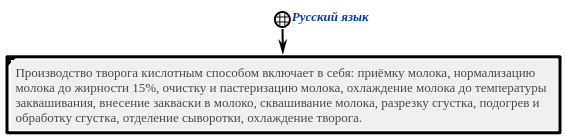
\includegraphics{Contents/part_kb/src/images/sd_natural_languages/nl_text.png}}
            \begin{scnindent}
            	\scntext{пояснение}{с точки зрения ostis-системы, любой естественно-языкой текст является \textit{файлом.}}
	            \scnrelfrom{лексическая структура}{\scnfileimage[20em]{Contents/part_kb/src/images/sd_natural_languages/nl_lexical.png}}
			    \begin{scnindent}
		            \scntext{пояснение}{Данная конструкция описывает декомпозицию исходного текста на фрагменты с указанием их принадлежности определённой \textit{номинативной единице} или \textit{знаку алфавита синтаксиса}.}
		            \scnrelfrom{синтаксическая структура}{\scnfileimage[20em]{Contents/part_kb/src/images/sd_natural_languages/nl_synactical.png}}
		            \scntext{пояснение}{Здесь приведена только частью синтаксической структуры. Оставшаяся часть записывается аналогично.}
		         \end{scnindent}
        	\end{scnindent}
        \end{scneqtoset}
    \end{scnsubstruct}
    \bigskip
    \scnendcurrentsectioncomment
\end{SCn}


\scparagraph{Пункт 44.1.1. Предметная область и онтология синтаксиса естественных языков}
\label{sd_syntax_natural_lang}
\begin{SCn}
    \scnsectionheader{Предметная область и онтология синтаксиса естественных языков}
    \begin{scnsubstruct}

        \scnsectionheader{Предметная область синтаксиса естественных языков}
        \begin{scnhaselementrolelist}{максимальный класс объектов исследования}
            \scnitem{синтаксис естественного языка}
        \end{scnhaselementrolelist}
        \begin{scnrelfromlist}{библиографическая ссылка}
            \scnitem{\scncite{Adger2003}}
            \scnitem{\scncite{Jackendoff1977}}
            \scnitem{\scncite{Haegeman1994}}
            \scnitem{\scncite{Carnie2012}}
        \end{scnrelfromlist}

        \scnheader{синтаксис естественного языка}
        \scntext{примечание}{Приводимая ниже формализация \textit{синтаксиса} \textit{естественных языков} является ядром, общим для всех \textit{естественных языков}. Очевидно, что \textit{синтаксис} некоторого конкретного \textit{естественного языка} может отличаться от \textit{синтаксиса} других \textit{языков}. В таком случае, более частные отличия необходимо отдельно специфицировать в формализованном виде. Таким образом, ниже будет предложено описание наиболее общих аспектов \textit{синтаксиса} всех \textit{естественных языков}, которое в дальнейшем может дополняться, если того требует конкретная реализация \textit{естественно-языкового интерфейса} какой-либо \textit{ostis-системы}. При этом любые дополнения, специфичные для некоторого конкретного \textit{естественного языка}, не должны противоречить ядру формализации \textit{синтаксиса} \textit{естественных языков}, приведенному в данном разделе.}
        \scntext{примечание}{При формализации синтаксиса в основном использовались стандартные положения генеративной грамматики.}
        \begin{scnindent}
            \begin{scnrelfromset}{источник}
                \scnitem{\scncite{Adger2003}}
                \scnitem{\scncite{Jackendoff1977}}
                \scnitem{\scncite{Haegeman1994}}
                \scnitem{\scncite{Carnie2012}}
            \end{scnrelfromset}
        \end{scnindent}

        \scnheader{грамматическая категория}
        \scntext{определение}{\textbf{\textit{грамматическая категория}} --- система противопоставленных друг другу рядов грамматических форм с однородными значениями.}
        \scntext{примечание}{В рамках нашей формализации предлагается представить грамматические категории как классы ролевых отношений, каждый из которых соответствует определенному грамматическому значению.
            \\Следует отметить, что приводятся основные \textit{грамматические категории}, часто встречающиеся в \textit{естественных языках}, а не всех возможные.}
        \scnhaselement{лицо}
        \begin{scnindent}
            \scnrelto{семейство подмножеств}{ролевое отношение}
            \scnhaselement{первое лицо\scnrolesign}
            \scnhaselement{второе лицо\scnrolesign}
            \scnhaselement{третье лицо\scnrolesign}
        \end{scnindent}
        \scnhaselement{число}
        \begin{scnindent}
            \scnrelto{семейство подмножеств}{ролевое отношение}
            \scnhaselement{единственное число\scnrolesign}
            \scnhaselement{множественное число\scnrolesign}
            \scnhaselement{двойственное число\scnrolesign}
            \scnhaselement{тройственное число\scnrolesign}
            \scnhaselement{паукальное число\scnrolesign}
        \end{scnindent}
        \scnhaselement{род}
        \begin{scnindent}
            \scnrelto{семейство подмножеств}{ролевое отношение}
            \scnhaselement{мужской род\scnrolesign}
            \scnhaselement{средний род\scnrolesign}
            \scnhaselement{женский род\scnrolesign}
        \end{scnindent}
        \scnhaselement{падеж}
        \begin{scnindent}
            \scnrelto{семейство подмножеств}{ролевое отношение}
            \scnhaselement{именительный падеж\scnrolesign}
            \scnhaselement{родительный падеж\scnrolesign}
            \scnhaselement{дательный падеж\scnrolesign}
            \scnhaselement{винительный падеж\scnrolesign}
            \scnhaselement{творительный падеж\scnrolesign}
            \scnhaselement{предложный падеж\scnrolesign}
            \scnhaselement{звательный падеж\scnrolesign}
            \scnhaselement{абсолютивный падеж\scnrolesign}
            \scnhaselement{эргативный падеж\scnrolesign}
        \end{scnindent}
        \scnhaselement{время}
        \begin{scnindent}
            \scnrelto{семейство подмножеств}{ролевое отношение}
            \scnhaselement{настоящее время\scnrolesign}
            \scnhaselement{прошедшее время\scnrolesign}
            \scnhaselement{будущее время\scnrolesign}
        \end{scnindent}
        \scnhaselement{наклонение}
        \begin{scnindent}
            \scnrelto{семейство подмножеств}{ролевое отношение}
            \scnhaselement{изъявительное наклонение\scnrolesign}
            \scnhaselement{повелительное наклонение\scnrolesign}
            \scnhaselement{сослагательное наклонение\scnrolesign}
            \scnhaselement{условное наклонение\scnrolesign}
        \end{scnindent}
        \scnhaselement{залог}
        \begin{scnindent}
            \scnrelto{семейство подмножеств}{ролевое отношение}
            \scnhaselement{действительный залог\scnrolesign}
            \scnhaselement{страдательный залог\scnrolesign}
            \scnhaselement{средний залог\scnrolesign}
            \scnhaselement{возвратный залог\scnrolesign}
            \scnhaselement{взаимный залог\scnrolesign}
        \end{scnindent}
        \scnhaselement{вид}
        \begin{scnindent}
            \scnrelto{семейство подмножеств}{ролевое отношение}
            \scnhaselement{совершенный вид\scnrolesign}
            \scnhaselement{несовершенный вид\scnrolesign}
            \scnhaselement{общий вид\scnrolesign}
            \scnhaselement{прогрессивный вид\scnrolesign}
            \scnhaselement{перфектный вид\scnrolesign}
        \end{scnindent}
        \scnhaselement{степень сравнения}
        \begin{scnindent}
            \scnrelto{семейство подмножеств}{ролевое отношение}
            \scnhaselement{положительная степень сравнения\scnrolesign}
            \scnhaselement{сравнительная степень сравнения\scnrolesign}
            \scnhaselement{превосходная степень сравнения\scnrolesign}
        \end{scnindent}

        \scnheader{часть речи}
        \scntext{определение}{\textbf{\textit{часть речи}} --- \textit{категория}, представляющая собой класс синтаксически эквивалентных \textit{знаков} \textit{естественного языка}.}
        \scnrelto{семейство подмножеств}{лексема}
        \scnhaselement{существительное}
        \scnhaselement{прилагательное}
        \scnhaselement{глагол}
        \scnhaselement{наречие}
        \scnhaselement{предлог}
        \scnhaselement{комплементатор}
        \scnhaselement{вспомогательный глагол}
        \scnhaselement{детерминант}

        \scnheader{словоформа}
        \scntext{определение}{\textbf{\textit{словоформа}} --- \textit{подмножество} \textit{лексемы}, которому принадлежат все вхождения \textit{лексемы} с определенными \textit{грамматическими значениями}.}
        \scntext{примечание}{В рамках нашей \textit{онтологии} словоформа понимается несколько иначе, чем принято в лингвистике, так как все вхождения лексемы в технологии OSTIS являются \textit{файлами}.}
        
        \scnheader{дистрибуция знака}
        \scntext{определение}{\textbf{\textit{дистрибуция знака}} --- это подмножество синтаксических правил, в которые входит данный \textit{знак}.}

        \scnheader{составляющая}
        \scntext{определение}{\textbf{\textit{составляющая}} --- элемент множества \textit{C} подмножеств кортежа вхождений лексем \textit{S}, которое содержит в качестве элементов как сам \textit{S}, так и все вхождения лексем в \textit{S}, таким образом, что любые два подмножества, входящие в \textit{C}, либо не пересекаются, либо одно из них включается в другое.}
        \scnrelfrom{пример}{Рисунок. Иллюстрация связей между составляющими}
        
        \scnheader{непосредственно составляющая}
        \scntext{определение}{\textbf{\textit{непосредственно составляющая}} ---  есть множество \textit{составляющих} \textit{S}, в которое входят \textit{составляющие} \textit{A} и \textit{B}. В является \textit{непосредственно составляющей} \textit{А} если и только если \textit{В} является подмножеством \textit{А} и нет такой \textit{составляющей} \textit{С}, которая является подмножеством \textit{А} и подмножеством которой является \textit{В}.}

        \scnheader{составляющие сестры*}
        \scntext{определение}{\textbf{\textit{составляющими сестрами*}} считаются \textit{составляющие}, являющиеся \textit{непосредственно составляющими} одной и той же \textit{составляющей}.}

        \scnheader{Рисунок. Иллюстрация связей между составляющими}
        \scneq{\scnfileimage[30em]{Contents/part_kb/src/images/sd_natural_languages/syntactic_example.png}}
        
        \scnheader{элементарная составляющая}
        \scntext{определение}{\textbf{\textit{элементарная составляющая}} --- элемент кортежа вхождений \textit{лексем} \textit{L}, являющихся \textit{непосредственно составляющими} множества \textit{составляющих} \textit{C} и не имеющих непосредственно составляющих \textit{составляющих}.}

        \scnheader{синтаксическая группа}
        \scntext{определение}{\textbf{\textit{синтаксическая группа}} --- класс \textit{составляющих}, в который входят \textit{составляющие} с вершинами, принадлежащими к одной \textit{части речи}.}
        \scntext{примечание}{\textit{синтаксические группы} представляют собой либо \textit{синглетон} (минимально включают в себя вершину), либо упорядоченную пару, состояющую из \textit{вершины} и другой \textit{синтаксической группы}.}

        \scnheader{вершина}
        \scntext{определение}{\textbf{\textit{вершина}} --- \textit{составляющая}, \textit{дистрибуция} которой совпадает с \textit{дистрибуцией} всей \textit{синтаксической группы}.}

        \scnheader{составляющая}
        \begin{scnrelfromset}{разбиение}
            \scnitem{синтаксическая группа}
            \scnitem{вершина}
        \end{scnrelfromset}
    
        \scnheader{синтаксическая группа}
        \begin{scnrelfromset}{разбиение}
            \scnitem{именная группа}
            \begin{scnindent}
                \scntext{определение}{\textit{именная группа} --- \textit{синтаксическая группа}, \textit{вершиной} которой является \textit{существительное}.}
            \end{scnindent}
            \scnitem{глагольная группа}
            \begin{scnindent}
                \scntext{определение}{\textit{глагольная группа} --- \textit{синтаксическая группа}, \textit{вершиной} которой является \textit{глагол}.}
            \end{scnindent}
            \scnitem{группа прилагательного}
            \begin{scnindent}
                \scntext{определение}{\textit{группа прилагательного} --- \textit{синтаксическая группа}, \textit{вершиной} которой является \textit{прилагательное}.}
            \end{scnindent}
            \scnitem{наречная группа}
            \begin{scnindent}
                \scntext{определение}{\textit{наречная группа} --- \textit{синтаксическая группа}, \textit{вершиной} которой является \textit{наречие}.}
            \end{scnindent}
            \scnitem{предложная группа}
            \begin{scnindent}
                \scntext{определение}{\textit{предложная группа} --- \textit{синтаксическая группа}, \textit{вершиной} которой является \textit{предлог}.}
            \end{scnindent}
            \scnitem{группа комплементатора}
            \begin{scnindent}
                \scntext{определение}{\textit{группа комплементатора} --- \textit{синтаксическая группа}, \textit{вершиной} которой является \textit{комплементатор}.}
            \end{scnindent}
            \scnitem{временная группа}
            \begin{scnindent}
                \scntext{определение}{\textit{временная группа} --- \textit{синтаксическая группа}, \textit{вершиной} которой является \textit{вспомогательный} либо \textit{модальный глагол}.}
            \end{scnindent}
            \scnitem{группа детерминанта}
            \begin{scnindent}
                \scntext{определение}{\textit{группа детерминанта} --- \textit{синтаксическая группа}, \textit{вершиной} которой является \textit{детерминант}.}
            \end{scnindent}
        \end{scnrelfromset}
        \begin{scnrelfromset}{разбиение}
            \scnitem{максимальная проекция вершины}
                \begin{scnindent}
                \scnidtf{максимальная проекция вершины синтаксической группы}
                \end{scnindent}
            \scnitem{промежуточная проекция вершины}
                \begin{scnindent}
                \scnidtf{промежуточная проекция вершины синтаксической группы}
                \end{scnindent}
        \end{scnrelfromset}

        \scnheader{максимальная проекция вершины группы детерминанта}
        \begin{scnreltoset}{пересечение}
            \scnitem{группа детерминанта}
            \scnitem{максимальная проекция вершины}
        \end{scnreltoset}
        \scntext{пояснение}{Могут быть введены более узкие классы, являющиеся пересечением приведенных выше, например \textit{максимальная проекция вершины группы детерминанта}.}

        \scnheader{SCg-текст. Иллюстрация синтаксической структуры предложения. Первая часть}
        \scneq{\scnfileimage[30em]{Contents/part_kb/src/images/sd_natural_languages/syntactic_structure_part_1.png}}
        \scntext{примечание}{Пример синтаксической структуры предложения}

        \scnheader{SCg-текст. Иллюстрация синтаксической структуры предложения. Вторая часть}
        \scneq{\scnfileimage[30em]{Contents/part_kb/src/images/sd_natural_languages/syntactic_structure_part_2.png}}
        \scntext{примечание}{Пример синтаксической структуры предложения}

        \scnheader{группа детерминанта}
        \begin{scnrelfromset}{пример}
            \scnfileitem{\textit{максимальная проекция вершины группы детерминанта} состоит из (\textit{максимальной проекции вершины группы детерминанта}) и \textit{промежуточной проекции вершины группы детерминанта}}
            \scnfileitem{\textit{промежуточная проекция вершины группы детерминанта} состоит из \textit{вершины группы детерминанта} (и \textit{максимальной проекции вершины именной группы})}
        \end{scnrelfromset}
        \begin{scnindent}
            \scntext{примечание}{В скобках указаны опциональные элементы.}
        \end{scnindent}

        \scnheader{именная группа}
        \begin{scnrelfromset}{пример}
            \scnfileitem{\textit{максимальная проекция вершины именной группы} состоит из (\textit{максимальной проекции вершины группы детерминанта}) и \textit{промежуточной проекции вершины именной группы}}
            \scnfileitem{\textit{промежуточная проекция вершины именной группы} состоит из (\textit{максимальной проекции вершины группы прилагательного}) и \textit{промежуточной проекции вершины именной группы} ИЛИ \textit{промежуточной проекции вершины именной группы} (и \textit{максимальной проекции вершины предложной группы})}
            \scnfileitem{\textit{промежуточная проекция вершины именной группы} состоит из \textit{вершины именной группы} (и \textit{максимальной проекции вершины предложной группы})}
        \end{scnrelfromset}
        \begin{scnindent}
            \scntext{примечание}{В скобках указаны опциональные элементы.}
        \end{scnindent}

        \scnheader{глагольная группа}
        \begin{scnrelfromset}{пример}
            \scnfileitem{\textit{максимальная проекция вершины глагольной группы} состоит из \textit{промежуточная проекция вершины глагольной группы}}
            \scnfileitem{\textit{промежуточная проекция вершины глагольной группы} состоит из \textit{промежуточной проекции вершины глагольной группы} (и \textit{максимальной проекции вершины предложной группы}) ИЛИ \textit{промежуточной проекции вершины глагольной группы} (и \textit{максимальной проекция вершины наречной группы})}
            \scnfileitem{\textit{промежуточная проекция вершины глагольной группы} состоит из \textit{вершины глагольной группы} (и \textit{максимальной проекции вершины именной группы})}
       \end{scnrelfromset}
        \begin{scnindent}
            \scntext{примечание}{В скобках указаны опциональные элементы.}
        \end{scnindent}

        \scnheader{наречная группа}
        \begin{scnrelfromset}{пример}
            \scnfileitem{\textit{максимальная проекция вершины наречной группы} состоит из \textit{промежуточной проекции вершины наречной группы}}
            \scnfileitem{\textit{промежуточная проекция вершины наречной группы} состоит из (\textit{максимальной проекции вершины наречной группы}) и \textit{промежуточной проекции вершины наречной группы}}
            \scnfileitem{\textit{промежуточная проекция вершины наречной группы} состоит из \textit{вершины наречной группы} (и \textit{максимальной проекции вершины предложной группы})}
       \end{scnrelfromset}
        \begin{scnindent}
            \scntext{примечание}{В скобках указаны опциональные элементы.}
        \end{scnindent}

        \scnheader{группа прилагательного}
        \begin{scnrelfromset}{пример}
            \scnfileitem{\textit{максимальная проекция вершины группы прилагательного} состоит из \textit{промежуточной проекции вершины группы прилагательного}}
            \scnfileitem{\textit{промежуточная проекция вершины группы прилагательного} состоит из (\textit{максимальной проекции вершины наречной группы}) и \textit{промежуточной проекции вершины группы прилагательного}}
            \scnfileitem{\textit{промежуточная проекция вершины группы прилагательного} состоит из \textit{вершины группы прилагательного} (и \textit{максимальной проекцим вершины предложной группы})}
       \end{scnrelfromset}
        \begin{scnindent}
            \scntext{примечание}{В скобках указаны опциональные элементы.}
        \end{scnindent}

        \scnheader{предложная группа}
        \begin{scnrelfromset}{пример}
            \scnfileitem{\textit{максимальная проекция вершины предложной группы} состоит из \textit{промежуточной проекции вершины предложной группы}}
            \scnfileitem{\textit{промежуточная проекция вершины предложной группы} состоит из \textit{промежуточной проекции вершины предложной группы} (и \textit{максимальной проекции вершины предложной группы}) ИЛИ (\textit{максимальной проекции вершины наречной группы}) и \textit{промежуточной проекции вершины предложной группы}}
            \scnfileitem{\textit{промежуточная проекция вершины предложной группы} состоит из \textit{вершины предложной группы} (и \textit{максимальной проекции вершины именной группы})}
        \end{scnrelfromset}
        \begin{scnindent}
            \scntext{примечание}{В скобках указаны опциональные элементы.}
        \end{scnindent}

        \scnheader{временная группа}
        \begin{scnrelfromset}{пример}
            \scnfileitem{\textit{максимальная проекция вершины временной группы} состоит из (\textit{максимальной проекции вершины группы детерминанта}) и \textit{промежуточной проекции вершины временной группы}}
            \scnfileitem{\textit{промГруппа комплементатораежуточная проекция вершины временной группы} состоит из \textit{вершины временной группы} (и \textit{максимальной проекции вершины глагольной группы})}
        \end{scnrelfromset}
        \begin{scnindent}
            \scntext{примечание}{В скобках указаны опциональные элементы.}
        \end{scnindent}

        \scnheader{группа комплементатора}
        \begin{scnrelfromset}{пример}
            \scnfileitem{\textit{максимальная проекция вершины группы комплементатора} состоит из (\textit{максимальной проекции вершины некоторой синтаксической группы}) и \textit{промежуточной проекции вершины группы комплементатора}}
            \scnfileitem{\textit{промежуточная проекция вершины группы комплементатора} состоит из \textit{вершины группы комплементатора} \textit{и максимальной проекции вершины временной группы}}
       \end{scnrelfromset}
        \begin{scnindent}
            \scntext{примечание}{В скобках указаны опциональные элементы.}
        \end{scnindent}

        \scnheader{структуры синтаксических групп}
        \scnrelfrom{пример}{SCg-текст. Иллюстрация синтаксической структуры предложения. Первая часть}
        \scnrelfrom{пример}{SCg-текст. Иллюстрация синтаксической структуры предложения. Вторая часть}
        \scntext{примечание}{Структуры синтаксических групп не являются произвольными --- элементы внутри группы могут граничить только с определенными множествами элементов.}
        \scnrelfrom{смотрите}{SCg-текст. Иллюстрация правила структуры синтаксической группы}
        \scntext{примечание}{Правила структуры синтаксических групп можно обобщить и свести к трем более абстрактным.
            \begin{itemize}
                \item Правило спецификатора: \textit{максимальная проекция вершины синтаксической группы} \textit{XP} состоит из (\textit{максимальной проекции вершины} \textit{YP}) \textit{промежуточной проекции вершины синтаксической группы} \textit{X'}
                \item Правило адъюнкта: \textit{промежуточная проекция вершины синтаксической группы} \textit{X'} состоит из \textit{промежуточной проекции вершины синтаксической группы} \textit{$\bm{X'_1}$} (и \textit{максимальной проекции вершины синтаксической группы} \textit{ZP}) ИЛИ из (\textit{максимальной проекции вершины синтаксической группы} \textit{ZP}) и \textit{промежуточной проекции вершины синтаксической группы} \textit{X'}.
                \item Правило комплемента: \textit{промежуточная проекция вершины синтаксической группы}  \textit{X'} состоит из \textit{вершины} \textit{X} (и \textit{максимальной проекции вершины синтаксической группы} \textit{WP}).
            \end{itemize}}

        \scnheader{SCg-текст. Иллюстрация правила структуры синтаксической группы}
        \scneq{\scnfileimage[20em]{Contents/part_kb/src/images/sd_natural_languages/tree_structure_rule.png}}

        \scnheader{комплемент}
        \scntext{определение}{\textbf{\textit{комплемент}} --- \textit{синтаксическая группа}, являющаяся сестрой вершины.}
        \scnrelfrom{правило}{правило комплемента}
        \begin{scnindent}
            \scntext{пример}{\scnfileimage[30em]{Contents/part_kb/src/images/sd_natural_languages/complement_rule.png}}
            \begin{scnindent}
                \scnidtf{SCg-текст. Правило комплемента}
            \end{scnindent}
        \end{scnindent}

        \scnheader{адъюнкт}
        \scntext{определение}{\textbf{\textit{адъюнкт}} --- \textit{синтаксическая группа}, являющаяся дочерью (\textit{непосредственно составляющей}) промежуточной проекции и сестрой промежуточной проекции вершины той же \textit{синтаксической группы}.}
        \scnrelfrom{правило}{правило адъюнкта}
        \begin{scnindent}
            \scntext{пример}{\scnfileimage[30em]{Contents/part_kb/src/images/sd_natural_languages/adjunct_rule.png}}
            \begin{scnindent}
                \scnidtf{SCg-текст. Правило адъюнкта}
            \end{scnindent}
        \end{scnindent}

        \scnheader{спецификатор}
        \scntext{определение}{\textbf{\textit{спецификатор}} --- \textit{синтаксическая группа}, являющейся дочерью максимальной проекции и сестрой промежуточной проекции.}
        \scnrelfrom{правило}{правило спецификатора}
        \begin{scnindent}
            \scntext{пример}{\scnfileimage[30em]{Contents/part_kb/src/images/sd_natural_languages/specifier_rule.png}}
            \begin{scnindent}
                \scnidtf{SCg-текст. Правило спецификатора}
            \end{scnindent}
        \end{scnindent}

    \end{scnsubstruct}
    \bigskip
    \scnendcurrentsectioncomment
\end{SCn}


\scparagraph{Пункт 44.1.2. Предметная область и онтология денотационной семантики естественных языков}
\label{sd_sem_natural_lang}
\begin{SCn}
    \scnsectionheader{Предметная область и онтология денотационной семантики естественных языков}
    \begin{scnsubstruct}

        \scnsectionheader{Предметная область денотационной семантики естественных языков}
        \begin{scnhaselementrolelist}{максимальный класс объектов исследования}
            \scnitem{денотационная семантика естественного языка}
        \end{scnhaselementrolelist}
        \begin{scnrelfromlist}{библиографическая ссылка}
            \scnitem{\scncite{Heim1998}}
            \scnitem{\scncite{Winter2016}}
            \scnitem{\scncite{Portner2008}}
        \end{scnrelfromlist}

        \scnheader{формализация денотационной семантики естественного языка}
        \scntext{определение}{Формализацией \textit{денотационной семантики} \textit{естественного языка} мы будем считать множество общих правил перехода от \textit{синтаксиса информационных конструкций} \textit{естественных языков} к \textit{смысловому представлению информации}, содержащейся в исходной \textit{информационной конструкции}.}
        \scntext{пояснение}{Предлагается вариант формализации \textit{денотационной семантики} \textit{естественных языков} в рамках \textit{Технологии OSTIS}, для составления которой использовались стандартные положения формальной семантики.}
        \begin{scnindent}
            \begin{scnrelfromset}{источник}
                \scnitem{\scncite{Heim1998}}
                \scnitem{\scncite{Winter2016}}
                \scnitem{\scncite{Portner2008}}
            \end{scnrelfromset}
        \end{scnindent}
        
        \scnheader{денотационная семантика естественного языка}
        \scntext{примечание}{\textit{Денотационная семантика} \textit{языка} специфицирует интерпретацию элементов \textit{синтаксиса} данного \textit{языка} и представляет собой множество формул, описывающих то, каким образом \textit{информационным конструкциям} \textit{языка} ставятся в соответствие обозначаемые ими сущности и конфигурации отношений между этими сущностями.}
        \scntext{примечание}{\textit{Денотационная семантика} \textit{естественных языков} должна обладать свойством композициональности --- то есть интерпретация всего высказывания должна выводиться из интерпретации отдельных его частей.
            \\Таким образом, необходимо предоставить формальное описание интерпретации элементов \textit{синтаксиса} \textit{естественного языка}, представленных в предыдущем разделе, а также описание правил совмещения интерпретации отдельных элементов для получения \textit{смысла} всего высказывания.}

        \scnheader{правила, реализующие \textit{денотационную семантику} \textit{языка}}
        \scntext{примечание}{Данные правила должны применяться последовательно и позволяют получить \textit{смысл} текста \textit{естественного языка} по его синтаксической структуре, \scnqq{поднимаясь} по дереву \textit{составляющих} от \textit{вершин} к \textit{максимальным проекциям}.}
        \scnhaselement{Правило интерпретации вершины группы прилагательного и вершины именной группы}
        \begin{scnindent}
            \scnrelfrom{пример}{SCg-текст. Правило интерпретации вершины группы прилагательного и вершины именной группы}
        \end{scnindent}
        \scnhaselement{Правило интерпретации максимальной проекции вершины именной группы}
        \begin{scnindent}
            \scnrelfrom{пример}{SCg-текст. Правило интерпретации максимальной проекции вершины именной группы}
        \end{scnindent}
        \scnhaselement{Правило интерпретации максимальной проекции вершины глагольной группы, содержащей непереходный глагол}
        \begin{scnindent}
            \scnrelfrom{пример}{SCg-текст. Правило интерпретации максимальной проекции вершины глагольной группы, содержащей непереходный глагол}
        \end{scnindent}
        \scnhaselement{Правило интерпретации максимальной проекции вершины группы детерминанта}
        \begin{scnindent}
            \scnrelfrom{пример}{SCg-текст. Правило интерпретации максимальной проекции вершины группы детерминанта}
        \end{scnindent}
        \scnhaselement{Правило интерпретации промежуточной проекции вершины временной группы}
        \begin{scnindent}
            \scnrelfrom{пример}{SCg-текст. Правило интерпретации промежуточной проекции вершины временной группы}
        \end{scnindent}
        \scnhaselement{Правило интерпретации максимальной проекции вершины временной группы}
        \begin{scnindent}
            \scnrelfrom{пример}{SCg-текст. Правило интерпретации максимальной проекции вершины временной группы}
        \end{scnindent}
        \scnhaselement{Правило интерпретации предложения с переходным глаголом}
        \begin{scnindent}
            \scnrelfrom{пример}{SCg-текст. Правило интерпретации предложения с переходным глаголом}
        \end{scnindent}

        \scnheader{SCg-текст. Правило интерпретации вершины группы прилагательного и вершины именной группы}
        \scneq{\scnfileimage[30em]{Contents/part_kb/src/images/sd_natural_languages/d_sem_1.png}}
        \scntext{примечание}{На \textit{SCg-текст. Правило интерпретации вершины группы прилагательного и вершины именной группы} приведено правило, по которому происходит интерпретация вершин \textit{именной группы} и \textit{группы прилагательного}.
            \\Смыслом таких вершин является класс, например: \textit{прилагательному} \scnqq{черный} соответствует множество черных объектов, а \textit{существительному} \scnqq{кот} --- множество котов.}

        \scnheader{SCg-текст. Правило интерпретации максимальной проекции вершины именной группы}
        \scneq{\scnfileimage[30em]{Contents/part_kb/src/images/sd_natural_languages/d_sem_2.png}}
        \scntext{примечание}{На \textit{SCg-текст. Правило интерпретации максимальной проекции вершины именной группы} приведено правило, по которому происходит интерпретация \textit{именной группы}, максимальная проекция которой включается в себя также группу прилагательного.
            \\Как говорилось выше, для применения данного правила необходимо предварительное применение правила, представленного на \textit{SCg-текст. Правило интерпретации вершины группы прилагательного и вершины именной группы}.
            \\Смыслом таких конструкций является класс, являющийся результатом \textit{пересечения} классов, полученных в результате интерпретации \textit{вершин} \textit{групп прилагательного} и \textit{именной группы} по отдельности.
            \\Например: \textit{черный кот} --- множество черных котов, пересечение множества котов и черных объектов.}
        %тут мы комбинируем смыслы прилагательного и существительного, которые входят в одну именную группу

        \scnheader{SCg-текст. Правило интерпретации максимальной проекции вершины глагольной группы, содержащей непереходный глагол}
        \scneq{\scnfileimage[30em]{Contents/part_kb/src/images/sd_natural_languages/d_sem_3.png}}
        \scntext{примечание}{На \textit{SCg-текст. Правило интерпретации максимальной проекции вершины глагольной группы, содержащей непереходный глагол} приведено правило, по которому происходит интерпретация \textit{глагольной группы}.
            \\Необходимость включения в посылку правила всей ветки глагольной группы объясняется ее необходимостью для определения типа \textit{глагола} --- данное правило предназначено для интерпретации непереходных \textit{глаголов}.
            \\\textit{смыслом} такой конструкции является класс \textit{действий}.}
        %тут мы задаем интерпретацию всей глагольной группы (макс проекции) только для непереходных глаголов. написать, что смотрим по всей структуре группы целиком, потому что для того, чтобы отличить непереходный от переходного нам нужна вся ветка глагольной группы в дереве целиком

        \scnheader{SCg-текст. Правило интерпретации максимальной проекции вершины группы детерминанта}
        \scneq{\scnfileimage[30em]{Contents/part_kb/src/images/sd_natural_languages/d_sem_4.png}}
        \scntext{примечание}{На \textit{SCg-текст. Правило интерпретации максимальной проекции вершины группы детерминанта} приведено правило, по которому происходит интерпретация \textit{группы детерминанта} с неопределенным артиклем.
            \\Смыслом такой конструкции является существование элемента класса, являющегося \textit{смыслом} входящей в состав данной \textit{группы детерминанта} \textit{именной группы}.}
        %тут задается интерпретация сочетания именной группы с артиклем (в данном случае неопределенным)

        \scnheader{SCg-текст. Правило интерпретации промежуточной проекции вершины временной группы}
        \scneq{\scnfileimage[30em]{Contents/part_kb/src/images/sd_natural_languages/d_sem_5.png}}
        \scntext{примечание}{На \textit{SCg-текст. Правило интерпретации промежуточной проекции вершины временной группы} приведено правило, по которому происходит интерпретация \textit{промежуточной проекции вершины временной группы}, состоящей из вспомогательного \textit{глагола} и полнозначного глагола.
            \\Вспомогательный \textit{глагол} в данном случае задет класс действий по времени (является ли оно запланированным, выполняемым, уже выполненным и так далее).}
        %тут задаем интерпретацию сочетания вспомогательного глагола и основного глагола. вспомогательный у нас соответствует классу действий по времени

        \scnheader{SCg-текст. Правило интерпретации максимальной проекции вершины временной группы}
        \scneq{\scnfileimage[30em]{Contents/part_kb/src/images/sd_natural_languages/d_sem_6.png}}
        %тут задаем интерпретацию для аргументной структуры непереходного глагола (сочетания подлежащего с непереходным глаголом)
        \scntext{примечание}{На \textit{SCg-текст. Правило интерпретации максимальной проекции вершины временной группы} приведено правило, по которому происходит интерпретация \textit{максимальной проекции вершины временной группы} на основе полученного на предыдущем шаге \textit{смысла} \textit{промежуточной проекции вершины временной группы} и \textit{смысла} \textit{максимальной проекции группы детерминанта}.}

        \scnheader{SCg-текст. Правило интерпретации предложения с переходным глаголом}
        \scneq{\scnfileimage[30em]{Contents/part_kb/src/images/sd_natural_languages/d_sem_7.png}}
        \scntext{примечание}{На \textit{SCg-текст. Правило интерпретации предложения с переходным глаголом} приведено правило, по которому происходит интерпретация \textit{максимальной проекции вершины группы комплементатора} на основе полученных на предыдущих шагах \textit{смыслов} более частных конструкций.
            \\Данным правилом задается интерпретация предложения с переходным \textit{глаголом}.}
        %тут задаем интерпретацию аргументной структуры переходного глагола (сочетания переходного глагола с его аргументами --- подлажещим и дополнением)

    \end{scnsubstruct}
    \bigskip
    \scnendcurrentsectioncomment
\end{SCn}


\scsubsubsection{\S 44.2. Предметная область и онтология синтаксического анализа естественно-языковых сообщений, входящих в ostis-систему}
\label{sd_process_syntax_message_analysis}
\begin{SCn}
    \scnsectionheader{Предметная область и онтология синтаксического анализа естественно-языковых сообщений, входящих в ostis-систему}
    \begin{scnsubstruct}
    \begin{scnrelfromlist}{соавтор}
        \scnitem{Никифоров С.А.}
        \scnitem{Гойло А.А.}
        \scnitem{Цянь Л.}
    \end{scnrelfromlist}

    \scnheader{Предметная область синтаксического анализа естественно-языковых сообщений, входящих в ostis-систему}
    \scntext{введение}{В данной предметной области не будет подробно описан процесс лексического анализа и его ключевые аспекты (такие как, например, устранение омонимии) --- данный вопрос требует дополнительной проработки. Вместо этого, акцент будет сделан на этап синтаксического анализа, предварительным условием которого является уже проведенный лексический анализ текста \textit{естественного языка}. Лексический анализ основывается на средствах введенных в Предметной области и онтологии синтаксиса естественных языков.}
    \begin{scnhaselementrolelist}{класс объектов исследования}
        \scnitem{лексический анализ}
        \scnitem{действие. лексический анализ естественно-языкового сообщения}
        \scnitem{лексема}
        \scnitem{единица сегментации}
        \scnitem{синтаксический анализ}
    \end{scnhaselementrolelist}

    \scnheader{действие. лексический анализ естественно-языкового сообщения}
    \begin{scnrelfromset}{обобщенная декомпозиция}
        \scnitem{действие. декомпозиция текста на токены}
        \scnitem{действие. сопоставление токенов с лексемами}
    \end{scnrelfromset}

    \scnheader{лексический анализ}
    \scntext{примечание}{С точки зрения \textit{ostis-системы}, любой \textit{естественно-языковой} текст является \textit{файлом}}
        \begin{scnindent}
            \scnrelfrom{источник}{Предметная область и онтология файлов, внешних информационных конструкций и внешних языков ostis-систем}
        \end{scnindent}
    \scntext{пояснение}{Лексический анализ представляет собой декомпозицию текста на последовательность токенов и сопоставление \textit{лексем} с получившимися при данной декомпозиции токенами. Следует отметить, что данные токены при необходимости могут сопоставляться не с \textit{лексемами}, а с их подмножествами, входящими в ее \textit{морфологическую парадигму}, соответствующими определенным грамматическим категориям: падежу, числу, роду и так далее.}
    \scnrelfrom{пример результата}{\scnfileimage[40em]{Contents/part_ui/src/images/sd_ui/lexical.png}}
    \begin{scnindent}
        \scnidtf{SCg-текст. Иллюстрация результата лексического анализа}
    \end{scnindent}
    \scntext{примечание}{Для осуществления лексического анализа, в базе знаний системы также должен присутствовать словарь, содержащий \textit{лексемы} и их различные формы.}
    
    \scnheader{лексема}
    \scntext{определение}{\textbf{\textit{лексема}} --- единица словарного состава языка, которая представляет собой множество всех форм некоторого слова}
    \scnrelfrom{пример спецификации}{SCg-текст. Иллюстрация к спецификации лексемы в базе знаний.}
    \begin{scnindent}
        \scnrelfrom{источник}{Предметная область и онтология естественных языков}
    \end{scnindent}

    \scnheader{единица сегментации}
	\scntext{определение}{базовая единица для обработки китайского языка, имеющая определенные семантические или грамматические свойства}
	\scnsubset{файл}
    \begin{scnrelfromlist}{примечание}
        \scnfileitem{В Предметной области и онтологии синтаксиса естественных языков предлагалась формализация лингвистических знаний, совместимых в первую очередь с европейскими языками. В данной предметной области мы также рассмотрим, как могут учитываться особенности конкретных естественных языков при разработке естественно-языковых интерфейсов ostis-систем на примере китайского языка.}
        \scnfileitem{Традиционно в лингвистике структура слова изучается в рамках морфологии. Носителем морфологической парадигмы и ключевым элементом анализа является лексема. Однако, в китайском языке из-за письменной традиции (текст китайского языка состоит из последовательности иероглифов без пробелов), наименьшей единицей при обработке текстов считается единица сегментации. Описание единицы сегмантации приводится в государственном стандарте «Стандарт сегментации слов современного китайского языка, используемый для обработки информации».}
        \scnfileitem{Стоит отметить, что термин единица сегментации используется при компьютерной обработке текстов китайского языка и не полностью совпадает с описанием слов в китайской лингвистике.}
        \scnfileitem{Кроме того, в китайском языке отсутствуют четкие показатели категорий числа, падежа и рода, в отличие от русского языка и других европейских языков. Функцию слова в китайском языке можно определить не на основании морфемного состава, а при помощи анализа связей этого слова с другими словами. В связи с этим, в процессе анализа текстов китайского языка сначала необходимо выполнить лексический анализ, разбивающий поток иероглифов в тексте китайского языка на отдельные значимые единицы сегментации.}
    \end{scnrelfromlist}
    \scnrelfrom{результат декомпозиции предложения на единицы сегментации}{\scnfileimage[40em]{Contents/part_ui/src/images/sd_ui/segment_chinese_sentence.png}}
    \begin{scnindent}
        \scnidtf{SCg-текст. Иллюстрация результата лексического анализа предложения на китайском языке}
    \end{scnindent}

    \scnheader{синтаксический анализ}
    \begin{scnrelfromvector}{примечание}
        \scnfileitem{Агент синтаксического анализа выполняет переход от размеченного на \textit{лексемы} текста к его \textit{синтаксической структуре}.}
        \begin{scnindent}
            \scnrelfrom{источник}{Предметная область и онтология информационных конструкций и языков}
        \end{scnindent}
        \scnfileitem{При этом из-за невозможности разрешения структурной неоднозначности на этапе синтаксического анализа, его результатом в общем случае будет являться множество потенциальных синтаксических структур.}
        \scnfileitem{Синтаксический анализ также основывается на средствах введенных в в Предметной области и онтологии синтаксиса естественных языков}
        \begin{scnindent}
            \begin{scnrelfromset}{пример синтексической структуры}
                \scnitem{SCg-текст. Иллюстрация синтаксической структуры предложения. Первая часть}
                \scnitem{SCg-текст. Иллюстрация синтаксической структуры предложения. Вторая часть}
            \end{scnrelfromset}
        \end{scnindent}
    \end{scnrelfromvector}

    \end{scnsubstruct}
\end{SCn}
    

\scsubsubsection{\S 44.3. Предметная область и онтология понимания естественно-языковых сообщений, входящих в ostis-систему}
\label{sd_process_message_understanding}
\begin{SCn}
    \scnsectionheader{Предметная область и онтология понимания естественно-языковых сообщений, входящих в ostis-систему}
    \begin{scnsubstruct}
    \begin{scnrelfromlist}{соавтор}
        \scnitem{Никифоров С.А.}
        \scnitem{Гойло А.А.}
        \scnitem{Цянь Л.}
    \end{scnrelfromlist}

    \scnheader{Предметная область понимания естественно-языковых сообщений, входящих в ostis-систему}
    \scnhaselementrole{максимальный класс объектов исследования}{действие. понимание естественно-языкового сообщения}
    \begin{scnhaselementrolelist}{класс объектов исследования}
        \scnitem{действие. разрешение контекста}
        \scnitem{действие. выбор смысла сообщения}
        \scnitem{действие. погружение сообщения в контекс}
        \scnitem{действие. переход от результата синтаксического анализа к потенциально эквивалентным сообщению структурам}
        \scnitem{смысл сообщении}
        \scnitem{контекст}
        \scnitem{контекст диалога}
        \scnitem{тематический контекст}
        \scnitem{пользовательский контекст}
        \scnitem{глобальный контекст}
        \scnitem{неизменяемый в ходе работы системы контекст диалога}
        \scnitem{изменяемый в ходе работы системы контекст диалога}
    \end{scnhaselementrolelist}

    \begin{scnhaselementrolelist}{исследуемое отношение}
        \scnitem{потенциально эквивалентная структура*}
        \scnitem{множество тематических контекстов диалога*}
    \end{scnhaselementrolelist}
    
    \scnheader{действие. понимание естественно-языкового сообщения}
    \begin{scnrelfromset}{обобщенная декомпозиция}
        \scnitem{действие. генерация вариантов значения сообщения}
        \begin{scnindent}
            \scntext{определение}{\textbf{\textit{действие. генерация вариантов значения сообщения}} --- \textit{действие}, в ходе которого осуществляется формирование \textit{строгой дизъюнкции} потенциально эквивалентных структур}
        \end{scnindent}
        \scnitem{действие. выбор и обновление контекста}
        \begin{scnindent}
            \begin{scnrelfromset}{обобщенная декомпозиция}
                \scnitem{действие. разрешение контекста}
                \scnitem{действие. выбор смысла сообщения на основе контекста}
                \scnitem{действие. погружение сообщения в контекст}
            \end{scnrelfromset}
        \end{scnindent}
    \end{scnrelfromset}

    \scnheader{потенциально эквивалентная структура*}
    \scntext{определение}{\textbf{\textit{потенциально эквивалентная структура*}} --- \textit{бинарное ориентированное отношение}, связывающее структуру и множество структур, которые потенциально могут быть эквивалентны ей, однако для достоверного определения факта требуются дополнительные \textit{действия}}
      
    \scnheader{правила перехода от результата синтаксического анализа к потенциально эквивалентным сообщению структурам}
    \scnrelfrom{источник}{Предметная область и онтология информационных конструкций и языков}
    \scnrelfrom{пример}{\scnfileimage[40em]{Contents/part_ui/src/images/sd_ui/transition_to_semanic_rule.png}}
    \begin{scnindent}
        \scnidtf{SCg-текст. Иллюстрация правила перехода от синтаксической структуры к семантике}
    \end{scnindent}
    
    \scnheader{действие. переход от результата синтаксического анализа к потенциально эквивалентным сообщению структурам}
    \begin{scnrelfromvector}{примечание}
        \scnfileitem{В результате действия перехода от результата синтаксического анализа к потенциально эквивалентным сообщению структурам в базе знаний формируется структура, описывающая возможные варианты смысла сообщения. Наличие нескольких таких структур объясняется тем, что в общем случае на этапе синтаксического анализа выполняется генерация нескольких вариантов синтаксической структуры. Выбор корректного значения сообщения будет осуществлен в ходе выполнения последующих действий.}
        \begin{scnindent}
            \scnrelfrom{источник}{\scncite{Jackendoff1977}}
            \scnrelfrom{смотрите}{SCg-текст. Иллюстрация конструкции, описывающей потенциальные смыслы сообщения}
        \end{scnindent}
        \scnfileitem{Следует отметить, что при необходимости смысл сообщения может быть сгенерирован не только на основании его синтаксической структуры в терминах грамматики составляющих, но и других знаний о данном сообщении, например выделенных из текста данного сообщения троек вида субъект-отношение-объект, результата его классификации и тому подобные.}
        \scnfileitem{Дальнейшие этапы процесса понимания сообщения выполняются на основе контекста.}
    \end{scnrelfromvector}

    \scnheader{смысл сообщении}
    \scnrelfrom{пример}{SCg-текст. Иллюстрация конструкции, описывающей потенциальные смыслы сообщения}
    
    \scnheader{SCg-текст. Иллюстрация конструкции, описывающей потенциальные смыслы сообщения}
	\scnrelfrom{иллюстрация}{\scnfileimage[40em]{Contents/part_ui/src/images/sd_ui/messsage_meaning_variants.png}}
    
    \scnheader{контекст диалога}
    \scnsubset{контекст}
    \begin{scnindent}
        \scntext{определение}{\textbf{\textit{контекст}} --- \textit{sc-структура}, содержащая знания, которыми оперирует система в ходе одного или нескольких диалогов}
        \begin{scnindent}
            \scntext{пояснение}{В общем случае, данные знания включают в себя как предварительно занесенные в \textit{базу знаний}, так и полученные в ходе работы с сенсоров и/или диалога.}
        \end{scnindent}
    \end{scnindent}
    \scnrelfrom{разбиение}{\scnkeyword{Типология контекстов диалога по глобальности\scnsupergroupsign}}
    \begin{scnindent}
        \begin{scneqtoset}
            \scnitem{тематический контекст}
            \scnitem{пользовательский контекст}
            \scnitem{глобальный контекст}
        \end{scneqtoset}
    \end{scnindent}
    \scnrelfrom{разбиение}{\scnkeyword{Типология контекство по сроку достоверности знаний\scnsupergroupsign}}
    \begin{scnindent}
        \begin{scneqtoset}
            \scnitem{неизменяемый в ходе работы системы контекст диалога}
            \scnitem{изменяемый в ходе работы системы контекст диалога}
        \end{scneqtoset}
    \end{scnindent}
    \scntext{примечание}{Подмножество \textit{контекста} может включаться в согласованную часть \textit{базы знаний}, например, если речь идет о каких-то предварительно занесенных в \textit{базу знаний} биографических сведениях --- дате рождения и тому подобном.}
    \scntext{прммечание}{В каждый момент времени с пользователем связан 1 пользовательский диалоговый контекст (содержащий, по крайней мере известные заранее факты о нем: имя, возраст и тому подобное) и несколько тематических.}
    \scnrelfrom{пример спецификации контекстов}{\scnfileimage[40em]{Contents/part_ui/src/images/sd_ui/user_context.png}}
    \begin{scnindent}
        \scnidtf{SCg-текст. Иллюстрация спецификации контекстов}
    \end{scnindent}
    \scntext{пояснение}{Актуальная информация собирается в тематический контекст, объединив который с контекстом пользователя и глобальным контекстом можно получить общий контекст, на основании которого должны осуществляться требуемые действия системы, включая генерацию ответа системы.}

    \scnheader{тематический контекст}
    \scntext{определение}{\textbf{\textit{тематический контекст}} --- \textit{контекст диалога}, содержащий специфические для темы сведения (сведения, полученные во время ведения диалога, на определенную тематику, например, при диалоге об определенном наборе сущностей)}

    \scnheader{множество тематических контекстов диалога*}
    \scntext{определение}{\textbf{\textit{множество тематических контекстов диалога*}} --- \textit{бинарное ориентированное отношение}, диалог с ориентированным множеством его тематических контекстов}

    \scnheader{пользовательский контекст}
    \scntext{определение}{\textbf{\textit{пользовательский контекст}} --- \textit{контекст диалога}, содержащие специфические для пользователя сведения, которые могут быть использованы в диалоге с ним на любую тематику}
    \scntext{примечание}{В общем случае пользовательский \textit{контекст} имеет пересечение с согласованной частью \textit{базы знаний} (предварительно занесенная в \textit{базу знаний} достоверная информация о пользователе, прошедшая необходимую модерацию), но не включается в нее целиком (часть, полученная в ходе диалога в которой мы не уверены).}
    \scnrelfrom{пример}{\scnfileimage[40em]{Contents/part_ui/src/images/sd_ui/context_in_KB.png}}
    \begin{scnindent}
        \scnidtf{Рисунок. Соотношение контекстов с согласованной частью баз знаний}
    \end{scnindent}

    \scnheader{глобальный контекст}
    \scntext{определение}{\textbf{\textit{глобальный контекст}} --- \textit{контекст диалога}, содержащий сведения, которые могут быть необходимы при ведении диалога с любым пользователем}
    \scntext{определение}{\textbf{\textit{глобальный контекст}} --- подмножество согласованной части \textit{базы знаний}, содержащее те сведения, что допустимо использовать в диалоге}
    \scntext{пример}{В диалоге с определенным пользователем не нужно использовать:
        \begin{itemize}
            \item находящуюся в базе знаний служебную информацию, необходимую для работы системы, но не предназначенную для использования в диалоге;
            \item части пользовательских контекстов иных пользователей.
        \end{itemize}}

    \scnheader{неизменяемый в ходе работы системы контекст диалога}
    \scntext{пояснение}{\textbf{\textit{Неизменяемый в ходе работы системы контекст диалога}} содержит в себе знания, необходимые для обеспечения выполнения системой своих функций,  которые были заложены в нее априорно ее разработчиками и/или администраторами и не изменяются в ходе ее функционирования на постоянной основе.}
    
    \scnheader{изменяемый в ходе работы системы контекст диалога}
    \scntext{пояснение}{\textbf{\textit{Изменяемый в ходе работы системы контекст диалога}} содержит в себе знания, необходимые для обеспечения выполнения системой своих функций,  которые были ей получены в ходе ее работы и/или достоверность которых скоротечна.}
    \scnrelfrom{разбиение}{\scnkeyword{Типология изменяемых в ходе работы системы контекстов по источнику знаний\scnsupergroupsign}}
    \begin{scnindent}
        \begin{scneqtoset}
            \scnitem{контекст диалога, содержащий знания из внешних источников}
            \scnitem{контекст диалога, содержащий знания, полученные в ходе диалога}
        \end{scneqtoset}
    \end{scnindent}
    \scnrelfrom{разбиение}{\scnkeyword{Типология изменяемых контекстов по степени их достоверности\scnsupergroupsign}}
    \begin{scnindent}
        \begin{scneqtoset}
            \scnitem{достоверный контекст диалога}
            \scnitem{недостоверный контекст диалога}
        \end{scneqtoset}
    \end{scnindent}

    \scnheader{действие. разрешение контекста}
    \scntext{примечание}{\textbf{\textit{действие. разрешение контекста}} сводится к сопоставлению каждому варианту его значения соответствующего \textit{контекста}. Выбор производится на основании значения функции \textit{$F\underscore{CTD}(T, C)$}, где \textit{T} --- \textit{вариант трансляции}, \textit{C} --- \textit{тематический контекст}. Подходящим контекстом для варианта трансляции считается тот, для которого значение этой функции максимально. В случае, если подходящий контекст не найден, генерируется новый.}
    \scnrelfrom{пример результата}{\scnfileimage[40em]{Contents/part_ui/src/images/sd_ui/relevant_contexts.png}}
    \begin{scnindent}
        \scnidtf{SCg-текст. Иллюстрация сообщения, всем вариантам значения которого сопоставлен контекст}
    \end{scnindent}

    \scnheader{действие. выбор смысла сообщения}
    \scntext{примечание}{\textbf{\textit{действие. выбор смысла сообщения}} представляет собой выбор из множества вариантов трансляции и соответствующих им \textit{контекстов} одной пары и обозначение ее как эквивалентной сообщению конструкции. В простейшем случае, на данном этапе допустимо выполнить выбор в соответствии с рассчитанными на предыдущем этапе для пар потенциально эквивалентных структур и соответствующих им \textit{контекстов} значениями функции \textit{$F\underscore{CTD}(T, C)$} и выбрать пару, для которой оно максимально, однако при необходимости также возможно введение и отдельной функции.}
	\scnrelfrom{пример результата}{\scnfileimage[40em]{Contents/part_ui/src/images/sd_ui/message_equivalent_structure.png}}
    \begin{scnindent}
        \scnidtf{SCg-текст. Иллюстрация конструкции, описывающей эквивалентную сообщению структуру}
    \end{scnindent}

    \scnheader{действие. погружение сообщения в контекс}
    \scntext{примечание}{\textbf{\textit{действие. погружение сообщения в контекст}} представляет собой погружение полученного смысла сообщения в \textit{контекст}. Кроме выбранного смысла сообщения, в контекст может добавляться и иная необходимая для обработки сообщения информация. Кроме того, на данном этапе на основе хранящихся в контексте сведений также должно выполняться разрешение местоимений.}
    \begin{scnrelfromset}{пример}
        \scnitem{SCg-текст. Иллюстрация контекста до погружения в него сообщения}
        \scnitem{SCg-текст. Иллюстрация контекста после погружения в него сообщения}
    \end{scnrelfromset}

    \scnheader{SCg-текст. Иллюстрация контекста до погружения в него сообщения}
    \scnrelfrom{иллюстрация}{\scnfileimage[40em]{Contents/part_ui/src/images/sd_ui/context_1.png}}

    \scnheader{SCg-текст. Иллюстрация контекста после погружения в него сообщения}
    \scnrelfrom{иллюстрация}{\scnfileimage[40em]{Contents/part_ui/src/images/sd_ui/context_2.png}}


    \end{scnsubstruct}
\end{SCn}
    


\scsubsubsection{\S 44.4. Предметная область и онтология синтеза естественно-языковых сообщений ostis-системы}
\label{sd_process_message_synthesis}
\begin{SCn}
    \scnsectionheader{Предметная область и онтология синтеза естественно-языковых сообщений ostis-системы}
    \begin{scnsubstruct}
    \begin{scnrelfromlist}{соавтор}
        \scnitem{Никифоров С.А.}
        \scnitem{Гойло А.А.}
        \scnitem{Цянь Л.}
    \end{scnrelfromlist}

    \scnheader{Предметная область синтеза естественно-языковых сообщений ostis-системы}
    \scnhaselementrole{максимальный класс объектов исследования}{методика разработки естественно-языковых интерфейсов}
    \begin{scnhaselementrolelist}{класс объектов исследования}
        \scnitem{методика разработки естественно-языковых интерфейсов}
        \scnitem{Библиотека многократно используемых компонентов естественно-языковых интерфейсов}
        \scnitem{Библиотека многократно используемых компонентов китайско-языкового интерфейса}
    \end{scnhaselementrolelist}
    
    \scnheader{методика разработки естественно-языковых интерфейсов}
    \scntext{примечание}{Методика разработки естественно-языковых интерфейсов включает несколько этапов, в которых необходимо учитывать методику построения и модификации гибридных баз знаний и гибридных решателей задач.}
    \begin{scnindent}
        \begin{scnrelfromlist}{источник}
            \scnitem{\scncite{Davydenko2018}}
            \scnitem{\scncite{Shunkevich2018}}
        \end{scnrelfromlist}
    \end{scnindent}
    \scnrelfrom{иллюстрация}{\scnfileimage[40em]{Contents/part_ui/src/images/sd_ui/method.png}}
    \begin{scnindent}
        \scnidtf{Рисунок. Этапы процесса разработки естественно-языкового интерфейса}
    \end{scnindent}
    \scntext{примечание}{Данная методика может быть применена при разработке конкретного естественно-языкового интерфейса по конкретной предметной области.}
    \begin{scnrelfromvector}{этапы}
        \scnitem{Этап 1. Формирование требований с учетом особенностей конкретного естественного языка}
        \begin{scnindent}
            \scntext{пояснение}{На данном этапе необходимо четко рассматривать особенности конкретного \textit{естественного языка}. Затем можно разработать базу знаний по обработке конкретного \textit{естественного языка} и соответствующие \textit{решатели задач} для выполнения обработки. После определения конкретного \textit{естественного языка} существует вероятность того, что в составе библиотеки компонентов уже есть реализованный вариант требуемой базы знаний и соответствующих решателей. В противном случае, тем не менее, у разработчика появляется возможность включить разработанную \textit{базу знаний} по обработке конкретного естественного языка и соответствующие \textit{решатели задач} в \textit{библиотеку компонентов} для последующего использования.}
        \end{scnindent}
        \scnitem{Этап 2. Разработка базы знаний по обработке конкретного естественного языка}
        \begin{scnindent}
            \scntext{пояснение}{На данном этапе при разработке базы знаний используются общие принципы согласованного построения и модификации \textit{гибридных баз знаний}.}
            \begin{scnindent}
                \scnrelfrom{источник}{\scncite{Davydenko2017}}
            \end{scnindent}
        \end{scnindent}
        \scnitem{Этап 3. Разработка решателей задач естественно-языковых интерфейсов}
        \begin{scnindent}
            \scntext{пояснение}{Для разработки \textit{решателей задач} \textit{естественно-языкового интерфейса}, направленных на приобретение фактографических знаний и генерацию текстов конкретного \textit{естественного языка}, используются общие принципы согласованного построения и модификации гибридных \textit{решателей задач}.}
            \begin{scnindent}
                \scnrelfrom{источник}{\scncite{Shunkevich2018}}
            \end{scnindent}
        \end{scnindent}
        \scnitem{Этап 4. Верификация разработанных компонентов}
        \begin{scnindent}
            \scntext{пояснение}{На данном этапе выполняется верификация разработанных \textit{компонентов} (\textit{базы знаний} по обработке конкретного естественного языка и соответствующего \textit{решателя задач}) конкретного \textit{естественно-языкового интерфейса}.}
        \end{scnindent}
        \scnitem{Этап 5. Отладка разработанных компонентов. Исправление ошибок}
    \end{scnrelfromvector}
    \begin{scnindent}
        \scntext{примечание}{Как правило, этапы 4 и 5 могут выполняться циклически до тех пор, пока разработанные компоненты не будут соответствовать предъявляемым требованиям.}
    \end{scnindent}

    \scnheader{Библиотека многократно используемых компонентов естественно-языковых интерфейсов}
	\begin{scnrelfromset}{разбиение}
		\scnitem{Библиотека многократно используемых компонентов базы знаний естественно-языковых интерфейсов}
		\begin{scnindent}
			\scnidtf{Библиотека многократно используемых компонентов лингвистической базы знаний}
			\scnidtf{Библиотека многократно используемых компонентов базы знаний по обработке естественного языка}
		\end{scnindent}
		\scnitem{Библиотека многократно используемых компонентов решателей задач естественно-языковых интерфейсов}
		\begin{scnindent}
			\scnidtf{Библиотека многократно используемых компонентов решателей задач для обработки естественного языка}
		\end{scnindent}
	\end{scnrelfromset}
    \scntext{примечание}{\textit{Библиотека многократно используемых компонентов} является важнейшим понятием в рамках \textit{Технологии OSTIS}. Библиотека многократно используемых компонентов естественно-языковых интерфейсов позволяет выбрать компоненты уже разработанные компоненты и включить их в разрабатываемый \textit{естественно-языковой интерфейс} других \textit{ostis-систем}, то есть разработанные компоненты \textit{естественно-языковых интерфейсов} могут быть повторно использованы при разработке естественно-языковых интерфейсов в других \textit{ostis-системах}. Ниже предложена структура библиотеки многократно используемых компонентов \textit{естественно-языковых интерфейсов}. При необходимости, библиотеку многократно используемых компонентов естественно-языковых интерфейсов можно дополнять знаниями о конкретных естественных языках.}
    \begin{scnindent}
        \scnrelfrom{источник}{Предметная область и онтология комплексной библиотеки многократно используемых семантически совместимых компонентов ostis-систем}
    \end{scnindent}

    \scnheader{Библиотека многократно используемых компонентов китайско-языкового интерфейса}
	\begin{scnrelfromset}{разбиение}
		\scnitem{Библиотека многократно используемых компонентов базы знаний китайско-языкового интерфейса}
		\begin{scnindent}
			\scnidtf{Библиотека многократно используемых компонентов базы знаний по обработке китайского языка}
		\end{scnindent}
		\scnitem{Библиотека многократно используемых компонентов решателей задач китайско-языкового интерфейса}
		\begin{scnindent}
			\scnidtf{Библиотека многократно используемых компонентов решателей задач для обработки китайского языка}
		\end{scnindent}
	\end{scnrelfromset}

    \end{scnsubstruct}
\end{SCn}
    


\scsubsubsection[
    \protect\scneditors{Захарьев В.А.;Азаров И.С.;Вашкевич М.И.;Крищенович В.А.;Жаксылык К.}
    \protect\scnmonographychapter{Глава 4.3. Аудиоинтерфейс ostis-систем}
    ]{Предметная область и онтология речевых интерфейсов современных интеллектуальных компьютерных системы}
\label{sd_ui_voice}
\begin{SCn}
\scnsectionheader{Предметная область и онтология речевых интерфейсов современных интеллектуальных компьютерных систем}
\begin{scnsubstruct}

\begin{scnrelfromlist}{автор}
    \scnitem{Захарьев В.А.}
    \scnitem{Азаров И.С.}
    \scnitem{Вашкевич М.И.}
    \scnitem{Крищенович В.А.}
    \scnitem{Жаксылык К.}
\end{scnrelfromlist}

\scnheader{Предметная область речевых интерфейсов современных интеллектуальных компьютерных систем}
\scniselement{предметная область}
\begin{scnhaselementrolelist}{класс объектов исследования}
    \scnitem{сигнал}
    \scnitem{аудиосигнал}
    \scnitem{речевой сигнал}
    \scnitem{модель сигнала}
    \scnitem{аудиоинтерфейс}
    \scnitem{речевой интерфейс}
\end{scnhaselementrolelist}

\scntext{аннотация}{Данная предметная область посвящена рассмотрению вопросов создания \textit{аудио} и \textit{речевых интерфейсов} для \textit{интеллектуальных компьютерных систем нового поколения}. Предлагается использование подхода на основе онтологического проектирования и формализации системы понятий. Изложены основные идеи, лежащие в основе данного подхода, а также их отличительные особенности от общепринятых. Показано, что в перспективе использование данного подхода может обеспечить свойства \textit{унификации}, \textit{семантической совместимости} и \textit{интероперабельности}, при разработке аудио и речевых интерфейсов, что в итоге позволит существенным образом сократить издержки при создании \textit{интеллектуальных компьютерных систем нового поколения} для решении \textit{комплексных задач}.}

\begin{scnrelfromvector}{конкатенация сегментов}
    \scnitem{Применение принципов онтологического проектирования при разработке аудиоинтерфейсов}
    \scnitem{Предметная область и онтология задач аудиоинтерфейса ostis-систем}
    \scnitem{Предметная область и онтология моделей параметрического представления сигнала}
\end{scnrelfromvector}

\begin{scnrelfromlist}{библиографическая ссылка}
    \scnitem{\scncite{Pearl2016}}
    \scnitem{\scncite{Chen2021audio}}
    \scnitem{\scncite{Lu2002content}}
    \scnitem{\scncite{Fernandes2022}}
    \scnitem{\scncite{Bellegarda2014}}
    \scnitem{\scncite{Lemley2017}}
    \scnitem{\scncite{Hoy2018}}
    \scnitem{\scncite{Semscholar2022stat}}
    \scnitem{\scncite{Popov2020interspeech}}
    \scnitem{\scncite{Povey2011ASRU}}
    \scnitem{\scncite{Deepa2021}}
    \scnitem{\scncite{Vosk2021}}
    \scnitem{\scncite{Radford2022robust}}
    \scnitem{\scncite{Delic2019speech}}
    \scnitem{\scncite{Standart2021}}
    \scnitem{\scncite{Davydenko2017}}
    \scnitem{\scncite{Shunkevich2018}}
    \scnitem{\scncite{Zahariev2018}}
    \scnitem{\scncite{Zahariev2019}}
    \scnitem{\scncite{Zahariev2020}}
    \scnitem{\scncite{Zahariev2021}}
    \scnitem{\scncite{Serra1990system}}
    \scnitem{\scncite{Griffin1988multiband}}
    \scnitem{\scncite{Petrovsky2011hybrid}}
    \scnitem{\scncite{Azarov2013instantaneous}}
    \scnitem{\scncite{Laroche1993hns}}
    \scnitem{\scncite{Mcaulay1986speech}}
    \scnitem{\scncite{Degottex2013mixed}}
    \scnitem{\scncite{Kawahara2010exploration}}
    \scnitem{\scncite{Kawahara2009development}}
    \scnitem{\scncite{ISO14496-3}}
    \scnitem{\scncite{ISO23003-3}}
    \scnitem{\scncite{IEEE1857-8}}
    \scnitem{\scncite{IEC62087-2}}
    \scnitem{\scncite{AES3250}}
\end{scnrelfromlist}

\begin{scnrelfromvector}{введение}
\scnfileitem{Разговорная речь является одной из наиболее естественных и эффективных форм передачи информации между людьми. Этот факт объясняет значительный интерес исследователей к вопросам развития и применения \textit{речевых интерфейсов} для обеспечения человеко-машинного взаимодействия в составе современных коммуникационных, мультимедийных и интеллектуальных систем.}
\begin{scnindent}
	\begin{scnrelfromset}{смотрите}
		\scnitem{\scncite{Chen2021audio}}
		\scnitem{\scncite{Pearl2016}}
	\end{scnrelfromset}
\end{scnindent}	
\scnfileitem{Более всеобъемлющей формой обеспечения взаимодействия с пользователем и окружающей средой посредством анализа и синтеза акустических сигналов является \textit{аудиоинтерфейс}. Данную разновидность интерфейса, выступающей родительской по отношению к речевым, можно кратко определить как аппаратно-программный комплекс осуществляющий анализ и синтез сигналов во всем доступном спектре параметров носителей акустической информации. Например, для решения задач анализа обстановки и событий происходящих в акустическом окружении системы, синтеза неречевых сигналов (звуков техногенного и природного характера, сигналов оповещения, музыки, и так далее).}
\begin{scnindent}
	\begin{scnrelfromset}{смотрите}
		\scnitem{\scncite{Lu2002content}}
	\end{scnrelfromset}
\end{scnindent}	
\scnfileitem{Об актуальности направления разработки аудио и речевых интерфейсов свидетельствуют следующие основные тенденции развития данного направления.}
\begin{scnindent}    
	\begin{scnrelfromset}{уточнение}
        \scnfileitem{Экономические показатели и прогнозы развития рынка речевых технологий, текущие среднегодовые темпы роста которого, по оценкам экспертов, составляют порядка 22\percent, а совокупный объем будет равен 59,6 млрд. долл. США к 2030.}
        \begin{scnindent}
        	\begin{scnrelfromset}{смотрите}
        		\scnitem{\scncite{Fernandes2022}}
        	\end{scnrelfromset}
        \end{scnindent}	
        \scnfileitem{Появление широкого спектра продуктов на основе речевого интерфейса, получивших массовое распространение. В первую очередь это персональные голосовые ассистенты, такие как \scnqq{Alexa} (Amazon), \scnqq{Siri} (Apple), \scnqq{Сortana} (MicroSoft), \scnqq{Алиса} (Yandex).}
        \begin{scnindent}
        	\begin{scnrelfromset}{смотрите}
        		\scnitem{\scncite{Bellegarda2014}}
        		\scnitem{\scncite{Lemley2017}}
        		\scnitem{\scncite{Hoy2018}}
        	\end{scnrelfromset}
        \end{scnindent}	
        \scnfileitem{Интерес со стороны научного сообщества, выражающийся в росте публикаций в этом направлении исследований на 15\percent за последние 5 лет.}
        \begin{scnindent}
        	\begin{scnrelfromset}{смотрите}
        		\scnitem{\scncite{Semscholar2022stat}}
        	\end{scnrelfromset}
        \end{scnindent}	
     \end{scnrelfromset}
\end{scnindent}
\scnfileitem{Необходимо отметить, что основная масса научных публикаций в данном направлении посвящена развитию базовых технологий, являющихся составляющими речевого интерфейса, таким как синтез речи по тексту, а также распознавание речи в текст. Последние достижения в этих направлениях связаны с бурным развитием нейросетевых моделей и вычислительных средств. Они позволили довести качественные характеристики использования речевых технологий до коммерческого уровня.}
\begin{scnindent}
	\begin{scnrelfromset}{смотрите}
		\scnitem{\scncite{Radford2022robust}}
		\scnitem{\scncite{Popov2020interspeech}}
		\scnitem{\scncite{Deepa2021}}
		\scnitem{\scncite{Povey2011ASRU}}
		\scnitem{\scncite{Vosk2021}}
	\end{scnrelfromset}
\end{scnindent}	
\scnfileitem{Большинство существующих систем, как правило, рассчитаны на решение определенного круга задач и сложно совместимы друг с другом. Данный факт в особенности остзличных \textit{моделей решения задач}. Такие системы, кроме стандартных модулей распознавания (ASро проявляется при проектировании сложных систем, наподобие интеллектуальных персональных диалоговых ассистентов, требующих использования многообразия различных видов обрабатываемой информации и раR, automatic speech recognition) и синтеза (TTS, text to speech), на уровне аудиоинтерфейса также должны содержать модели, определяющие наличие/отсутствие речи в аудиосигнале в сложной акустической обстановке, классификации звуков окружающей среды, распознавание диктора и пр. Помимо этого элементы речевого интерфейса должны быть совместимы с более высокоуровневыми модулями обработки естественно-языковой информации, такими как модули понимания (SLU, spoken language understanding) и генерации речи (SLG, spoken language generation), управления диалогом (DM, dialog manager).} 
\begin{scnindent}
	\begin{scnrelfromset}{смотрите}
		\scnitem{\scncite{Delic2019speech}}
	\end{scnrelfromset}
	\scnrelfrom{пример}{\scnfileimage[40em]{Contents/part_ui/src/images/sd_ui/ch43_fig01_speech-hmi-components.png}}
    \begin{scnindent}
        \scnidtf{Рисунок. Компоненты системы человеко-машинного речевого диалога}
        \scnrelfrom{смотрите}{\cite{Delic2019speech}}
    \end{scnindent}
\end{scnindent}	
\scnfileitem{Все это требует разработки подходов, основанных не только на методах машинного обучения и обработке сигналов, но и на обработке естественного языка, символических методах искусственного интеллекта, онтологическом проектировании и формализации предметной области аудиоинтерфейса. Это позволит создать системы, которые обладают полным спектром знаний в формализованном виде о типах задач, которые они должны решать, и методах, доступных для их решения.}
\scnfileitem{Необходимым условием для создания таких систем нового поколения, обладающих улучшенными характеристиками по критериям \textit{интероперабельности} и \textit{гибкости} является также тот факт, что данные системы должны быть построены на основе базовой технологии, позволяющей обеспечить такое единство формы представления информации на всех ее уровнях.}
\scnfileitem{Совокупность данных факторов приводит к необходимости создания \textit{интеллектуальных компьютерных систем нового поколения}, которые будут включать в себя модули аудио и речевого интерфейса, построенные на основе принципов интероперабельности и семантической совместимости для решения \textit{комплексных задач}.}
\end{scnrelfromvector}

\scnsectionheader{Применение принципов онтологического проектирования при разработке аудиоинтерфейсов}
\begin{scnsubstruct}
	
\scnheader{онтологическое проектирование при разработке аудиоинтерфейсов}
\begin{scnrelfromvector}{принципы, лежащие в основе}
	\scnfileitem{Для разработки аудиоинтерфейсов предлагается прибегнуть к подходу на основе принципов, лежащих в основе \scnqqi{Стандарта открытой технологии онтологического проектирования, производства и эксплуатации семантически совместимых гибридных интеллектуальных компьютерных систем} или кратко \scnqqi{Стандарта технологии OSTIS}.}
	\scnfileitem{Суть подхода заключается в рассмотрении процесса проектирования аудиоинтерфейса как интерфейсной подсистемы в рамках общего процесса разработки \textit{интеллектуальной компьютерной системы} и построении ее формальной \textit{логико-семантической модели}.}
	\scnfileitem{Необходимо создать подобную модели интеллектуальной компьютерной системы нового поколения.}
	\begin{scnindent}    
		\begin{scnrelfromlist}{требование}
		    \scnfileitem{Произведение декомпозиции информационной компьютерной системы на компоненты.}
		    \begin{scnindent} 
		    	\scntext{примечание}{Качество декомпозиции при этом определяется простотой последующего синтеза общей формальной модели из формальных моделей выделенных компонентов.}
		    \end{scnindent} 
		    \scnfileitem{Произведение \textit{конвергенции} выделенных компонентов в целях построения совместимых (легко интегрируемых) формальных моделей этих компонентов.}
		    \scnfileitem{Интеграция построенных формальных моделей выделенных компонентов и получение общей \textit{формальной модели}.}
		    \scnfileitem{В качестве технологической основы для реализации предлагаемого подхода будет использоваться Технология OSTIS, соответственно подсистема аудиоинтерфейса будет строиться как \textit{многократно используемый компонент}, который в будущем будет при необходимости встраиваться в различные ostis-системы.}
	    \end{scnrelfromlist}
	\end{scnindent}
\end{scnrelfromvector}

\scnheader{Технология OSTIS}
\begin{scnrelfromlist}{преимущество}
\scnfileitem{В рамках указанной технологии предложены унифицированные средства представления различных видов знаний, в том числе --- \textit{метазнаний}, что позволяет описать всю необходимую для анализа информацию в одной базе знаний в едином ключе.}
\begin{scnindent}
	\begin{scnrelfromset}{смотрите}
		\scnitem{\scncite{Davydenko2017}}
	\end{scnrelfromset}
\end{scnindent}	
\scnfileitem{Используемый в рамках технологии формализм позволяет специфицировать в базе знаний не только понятия, но и любые внешние с точки зрения базы знаний файлы (например, фрагменты речевого сигнала), в том числе --- синтаксическую структуру таких файлов.}
\scnfileitem{Предложенный в рамках технологии подход к представлению различных видов знаний и моделей их обработки обеспечивает модифицируемость ostis-систем, то есть позволяет легко расширять функциональные возможности системы, вводя новые виды знаний (новые системы понятий) и новые модели обработки знаний.}
\begin{scnindent}
	\begin{scnrelfromset}{смотрите}
		\scnitem{\scncite{Davydenko2017}}
		\scnitem{\scncite{Shunkevich2018}}
	\end{scnrelfromset}
\end{scnindent}	
\end{scnrelfromlist}
\begin{scnindent}
	\scntext{примечание}{Более подробно принципы построения комплексной технологии разработки и поддержки жизненного цикла \textit{интеллектуальных компьютерных систем нового поколения} --- \textit{Технологии OSTIS} --- изложены в \textit{Интеллектуальных компьютерных системах нового поколения}.}
	\scnrelfrom{смотрите}{Интеллектуальные компьютерные системы нового поколения}
\end{scnindent}

\scntext{особенность}{В отличие от различных работ авторов, посвященных вопросам семантического анализа голосовых сообщений на основе формализованного контекста и создания диалоговых ассистентов на основе модели ментального лексикона или мультимодальной системы на основе нейросимволического подхода, Технология OSTIS используется для непосредственного построения онтологии подсистем аудио интерфейса.}
\begin{scnindent}
	\begin{scnrelfromset}{смотрите}
		\scnitem{\scncite{Zahariev2019}}
		\scnitem{\scncite{Zahariev2020}}
		\scnitem{\scncite{Zahariev2021}}
		\scnitem{\scncite{Zahariev2018}}
	\end{scnrelfromset}
\end{scnindent}	

\scnheader{аудиоинтерфейс интеллектуальных компьютерных систем нового поколения}
\scntext{сокращение}{аудиоинтерфейс \textit{интеллектуальных компьютерных систем}}
\begin{scnrelfromset}{обобщенная декомпозиция}
    \scnitem{база знаний подсистемы аудиоинтерфейса \textit{интеллектуальных компьютерных систем нового поколения}}
    \scnitem{решатель задач подсистемы аудиоинтерфейса \textit{интеллектуальных компьютерных систем нового поколения}}
    \scnitem{интерфейс для взаимодействия с остальными интерфейсными подсистемами ostis-системы}
\end{scnrelfromset}
\scntext{примечание}{\textit{аудиоинтерфейс} \textit{интеллектуальных компьютерных систем нового поколения} должен иметь архитектуру, соответствующую общим правилам построения ostis-систем.}
\scntext{примечание}{Согласно общим принципам организации интерфейсов ostis-систем, изложенным в \textit{Общих принципах организации интерфейсов ostis-систем}, \textit{аудио- и речевой интерфейс} относятся к подмножеству \textit{SILK-интерфейсов} \textit{пользовательских интерфейсов} \textit{интеллектуальных компьютерных систем}.}

\scnheader{пользовательский интерфейс}
\scntext{принцип реализации}{Для решения задачи построения пользовательского интерфейса в базе знаний пользовательского интерфейса ostis-системы необходимо наличие \textit{sc-модели} компонентов \textit{пользовательского интерфейса}, интерфейсных действий пользователей, а также классификации пользовательских интерфейсов в целом. При проектировании интерфейса используется компонентный подход, который предполагает представление всего интерфейса приложения в виде отдельных \textit{специфицированных компонентов}, которые могут разрабатываться и совершенствоваться независимо.
	\\Процесс разработки аудиоинтерфейса для \textit{интеллектуальных компьютерных систем нового поколения}, подразумевает прежде всего создание семантически структурированных баз знаний в виде иерархической системы предметных областей и соответствующих им онтологий, специфицирующих эти предметные области. Следовательно, первым шагом для достижения поставленной цели должен являться этап выделения и формализации сущностей аудио и речевого интерфейса для погружения данной информации в базу знаний интеллектуальной компьютерной системы.}

\scnheader{Предметная область и онтология аудиоинтерфейса интеллектуальных компьютерных систем нового поколения}
\begin{scnrelfromset}{декомпозиция}
    \scnitem{Предметная область и онтология задач аудиоинтерфейса}
    \scnitem{Предметная область и онтология моделей параметрического представления сигнала}
\end{scnrelfromset}
\begin{scnindent}
\scntext{примечание}{В онтологию положен функциональный подход к декомпозиции предметных областей, что является вполне естественным, поскольку соответствует природе задач, реализуемых аудиоинтерфейсом.}
\end{scnindent}  
\end{scnsubstruct}
\scntext{вывод}{Представленные принципы в совокупности позволяют осуществлять конвергенцию и интеграцию компонентов как на уровне подсистемы аудиоинтерфейса, так и на уровне всей \textit{интеллектуальной компьютерной системы нового поколения} в целом, что, в свою очередь, позволяет перевести \textit{интеллектуальную информационную систему} в класс гибридных, \textit{интероперабельных} и \textit{семантически совместимых систем}.}

\scnsectionheader{Предметная область и онтология задач аудиоинтерфейса ostis-систем}
\begin{scnsubstruct}
	\scntext{примечание}{Первым шагом на пути к построению базы знаний подсистемы аудиоинтерфейса \textit{интеллектуальных компьютерных систем нового поколения} является формализация онтологии верхнего уровня. В основе данной онтологии предлагается положить формализованное представление основных сущностей предметной области и их свойств, а также функциональных задач, которые аудио и речевой интерфейс призваны решать.}
	\begin{scnhaselementrolelist}{класс объектов исследования}
		\scnitem{сигнал}
		\scnitem{аудиосигнал}
		\scnitem{речевой сигнал}
		\scnitem{акустический сигнал}
	\end{scnhaselementrolelist}
	\begin{scnindent}  
		\scntext{примечание}{Одним из ключевых понятий, требующих формализации, является базовое определение самого сигнала, а также основных разновидностей сигналов, в зависимости от их природы представляющих наибольший интерес в области аудиоинтерфейсов.}
	\end{scnindent}  

    \begin{scnhaselementrolelist}{класс объектов исследования}
        \scnitem{аналоговый сигнал}
        \scnitem{дискретный сигнал}
        \scnitem{цифровой сигнал}
        \scnitem{периодический сигнал}
        \scnitem{апериодический сигнал}
        \scnitem{гармонический сигнал}
        \scnitem{тональный сигнал}
        \scnitem{шумовой сигнал}
        \scnitem{импульсный сигнал}
    \end{scnhaselementrolelist}
    \begin{scnindent}  
        \scntext{примечание}{Классы выделены в зависимости от способа математического описания обрабатываемого сигнала в ostis-системе.}
    \end{scnindent}  
 
\begin{scnhaselementrolelist}{класс объектов исследования} 
    \scnitem{амплитуда сигнала}
    \scnitem{частота сигнала}
    \scnitem{фаза сигнала}
    \scnitem{интенсивность сигнала}
    \scnitem{длительность сигнала}
    \scnitem{мощность/энергия сигнала}
    \scnitem{осцилограмма сигнала}
    \scnitem{спектр сигнала}
    \scnitem{частота дискретизации сигнала}
    \scnitem{степень квантования сигнала}
\end{scnhaselementrolelist}
  \begin{scnindent}  
	\scntext{примечание}{Понятия, связанные с характеристиками самого сигнала, по основным его атрибутам.}
	\begin{scnindent}  
		\scnrelfrom{пример}{\scnfileimage[40em]{Contents/part_ui/src/images/sd_ui/ch43_fig02_speech-structure-segment-suprasegment.png}}
		\begin{scnindent}
			\scnidtf{Рисунок. Сегментные и надсегментные характеристики речевого сигнала}
		\end{scnindent}
	\end{scnindent} 
\end{scnindent}  
 
\begin{scnhaselementrolelist}{класс объектов исследования} 
    \scnitem{анализ аудиосигнала}
    \scnitem{синтез аудиосигнала}
    \scnitem{кодирование аудиосигнала}
    \scnitem{шумоочистка аудиосигнала}
    \scnitem{классификация аудиосигнала}
    \scnitem{классификация событий}
     \begin{scnindent}
    	\scnidtf{Enviromental Sound Classification, Acoustic Scenes and Events}
    \end{scnindent}
    \scnitem{детектирование аномалий}
    \begin{scnindent}
    	\scnidtf{Anomalous Sound Detection}
    \end{scnindent}
    \scnitem{идентификация положения источника в пространстве}
    \begin{scnindent}
    	\scnidtf{Sound Source Localization}
    \end{scnindent}
\end{scnhaselementrolelist}
\begin{scnindent}  
	\scntext{примечание}{Понятия предметной области, лежащие в семантической окрестности подпространства функционального назначения аудиоинтерфейсов и обработки аудиосигналов.}
\end{scnindent}

\begin{scnhaselementrolelist}{класс объектов исследования} 
    \scnitem{характеристики речевого сигнала}
    \scnitem{лингвистические характеристики сигнала}
    \scnitem{паралингвистические характеристики сигнала}
    \scnitem{экстралингвистические характеристики сигнала}
    \scnitem{сегментная характеристика речевого сигнала}
    \begin{scnindent}
    	\scnidtf{Segmantal Features}
    \end{scnindent}
    \scnitem{надсегментная характеристика речевого сигнала}
    \begin{scnindent}
    	\scnidtf{Suprasegmental Features}
    \end{scnindent}
    \scnitem{громкость речевого сигнала}
    \scnitem{тембр речевого сигнала}
    \scnitem{темп речевого сигнала}
    \scnitem{частота основного тона сигнала}
    \scnitem{фонемный состав речевого сигнала}
\end{scnhaselementrolelist} 
\begin{scnindent}  
	\scntext{примечание}{Основные понятия аудио и речевого интерфейса также тесно связаны с основными его характеристиками, которые можно разделить на основные группы понятий.}
	\scnrelfrom{смотрите}{\scncite{Okko2022}}
    \scnrelfrom{пример}{Рисунок. Сегментные и надсегментные характеристики речевого сигнала}
\end{scnindent}

\begin{scnhaselementrolelist}{класс объектов исследования}  
    \scnitem{анализ речевого сигнала}
    \scnitem{детектирование наличия ключевых слов}
    \begin{scnindent}
    	\scnidtf{Key Words Spotting}
    \end{scnindent}
    \scnitem{активация по ключевому слову}
    \begin{scnindent}
    	\scnidtf{Wake Up Word Detection}
    \end{scnindent}
    \scnitem{детектирование наличия речевого сигнала}
    \begin{scnindent}
    	\scnidtf{Voice Activity Detection}
    \end{scnindent}
    \scnitem{синтез речевого сигнала}
    \scnitem{синтез текста в речь}
    \begin{scnindent}
    	\scnidtf{Text-to-Speech Synthesis}
    \end{scnindent}
    \scnitem{эмоциональный синтез текста в речь}
    \begin{scnindent}
    	\scnidtf{Emotional Text-to-Speech Syntehsis}
    \end{scnindent}
    \scnitem{cинтез пения}
    \begin{scnindent}
    	\scnidtf{Sing Synthesis}
    \end{scnindent}
    \scnitem{распознавание эмоций в речевом сигнале}
    \begin{scnindent}
    	\scnidtf{Emotional Speech Recognition}
    \end{scnindent}
    \scnitem{распознавание диктора}
    \scnitem{сепарация речи}
    \begin{scnindent}
    	\scnidtf{speech diarization}
        \scnidtf{speech separation}
    \end{scnindent}
    \scnitem{классификация диктора}
    \begin{scnindent}
    	\scnidtf{Speaker Recognition}
    \end{scnindent}
    \scnitem{верификация диктора}
    \begin{scnindent}
    	\scnidtf{Speaker Verification}
    \end{scnindent}
\end{scnhaselementrolelist}
\begin{scnindent}  
	\scntext{примечание}{Основные понятия предметной области, лежащие в семантической окрестности функционального назначения речевого сигнала и обработки аудиосигналов.}
\end{scnindent}

\scntext{примечание}{Необходимо отметить, что вышеобозначенные понятия зачастую сложным и нетривиальным образом связаны между собой в процессе перехода от источников информации к непосредственным физическим параметрам. Такую сложную структуру сигнала можно представить в виде схемы его информационной структуры. Этот факт требует от \textit{интеллектуальных компьютерных систем нового поколения} формализации понятий для того, чтобы система могла автоматически интерпретировать взаимосвязи между данными характеристиками при работе с аудио и речевыми сигналами. И, как следствие, выдать ответ пользователю, объясняющий на основе каких характеристик система пришла к тому или иному выводу.}
\begin{scnindent}
	\scnrelfrom{смотрите}{\scnfileimage[40em]{Contents/part_ui/src/images/sd_ui/ch43_fig03_speech-signal-inf-structure-ru.png}}
	\begin{scnindent}
	    \scnidtf{Рисунок. Информационная структура речевого сигнала}
	\end{scnindent}
	\scnrelfrom{смотрите}{\scncite{Lobanov2006}}
\end{scnindent}

\scnheader{и.к.с нового поколения}
\scntext{примечание}{Для построения \textit{интеллектуальных компьютерных систем нового поколения} в фокусе лежат задачи, связанные с обработкой речевых сигналов, решение которых необходимо в первую очередь для построения речевого интерфейса.}
\scntext{примечание}{Основу \textit{sc-модели базы знаний} составляет иерархическая система предметных областей и соответствующих им онтологий.}
\scntext{примечание}{В зависимости от модели представления сигнала в ostis-системе также могут быть определены различные описания основных видов сигналов, применение которых обосновано особенностями природы анализируемого сигнала, а также решаемой задачей анализа.}
\begin{scnindent}  
	\scnrelfrom{смотрите}{математическая модель сигнала}
\end{scnindent} 
\scntext{примечание}{Важным аспектом в процессе проектирования является формализация \textit{классов задач} аудиоинтерфейса, поскольку благодаря этим знаниям в интеллектуальной системе могут (и должны) применяться соответствующие методы обработки, в зависимости от типа решаемой задачи.}
\begin{scnindent}
 	\scnrelfrom{смотрите}{\scnfileimage[40em]{Contents/part_ui/src/images/sd_ui/ch43_fig04_audio-and-speech-tasks-formalization-ru.png}}
 	\begin{scnindent}
 		\scnidtf{SCg-текст. Фрагмент онтологии верхнего уровня задач аудио- и речевых интерфейсов для интеллектуальных компьютерных систем нового поколения}
 		\scntext{примечание}{Фрагмент онтологии верхнего уровня типовых \textit{задач} решаемых \textit{интеллектуальной компьютерной системой} в области обработки аудио- и речевых сигналов.}
 	\end{scnindent}
\end{scnindent}
 
\scnheader{сигнал}
\scntext{определение}{сигнал --- это физический процесс, несущий сообщение (информацию) о каком-либо событии, состоянии объекта наблюдения либо передающий команды управления, оповещения и так далее.}
\scnsuperset{акустический сигнал}
\begin{scnindent}
    \scntext{определение}{акустический сигнал --- это сигнал, представляющий собой распространение упругих волн в газообразной, жидкой или твердой среде.}
\end{scnindent}
\scnsuperset{аудиосигнал}
\begin{scnindent}
    \scnidtf{слышимый звуковой сигнал}
    \scntext{определение}{аудиосигнал --- это акустический сигнал, параметры которого находятся в пределах диапазона значений доступного для восприятия органами чувств человека.}
    \scnsuperset{акустический сигнал}
    \scntext{примечание}{Диапазон частот аудиосигнала лежит в интервале от 20 до 20 000 Гц.}
\end{scnindent}
\scnsuperset{речевой сигнал}
\begin{scnindent}
	\scntext{определение}{речевой сигнал --- это аудиосигнал, который образуется в результате прохождения воздушных потоков через речевой тракт человека. В результате всевозможных акустических преобразований происходит формирование различных звуков речи.}
	\scnhaselement{устная речь}
	\scnhaselement{речеобразование}
	\scntext{примечание}{Механизм речеобразования человека представляет собой акустическую трубу с динамически изменяющимися параметрами поперечного сечения, возбуждаемую либо квазипериодической последовательностью импульсов, генерируемых голосовыми связками, либо турбулентным потоком воздуха, проталкиваемого сквозь сужения, в разных местах речевого тракта.}
\end{scnindent}

\scnheader{математическая модель сигнала}
\begin{scnreltoset}{объединение}
    \scnitem{аналоговый сигнал}
	\begin{scnindent}
	\scntext{определение}{аналоговый сигнал --- сигнал параметры которого можно измерить в любой момент времени.}
    \scntext{определение}{аналоговый сигнал --- сигнал, у которого каждый из представленных параметров описывается функцией времени и непрерывным множеством возможных значений.}
    \end{scnindent}
    \scnitem{дискретный сигнал}
	\begin{scnindent}
	\scntext{определение}{дискретный сигнал --- сигнал, у которого хотя бы один из представленных параметров описывается конечным множеством возможных значений.}
	\begin{scnreltoset}{объединение}
	    \scnitem{дискретный по времени}
        \scnitem{дискретный по амплитуде}
    \end{scnreltoset}
    \end{scnindent}
    \scnitem{цифровой сигнал}
	\begin{scnindent}
	\scntext{определение}{цифровой сигнал --- сигнал, у которого каждый из представляющих параметров описывается функцией дискретного времени и конечным множеством возможных значений.}
	\begin{scnrelfromset}{включает}
    \scnitem{дискретный по времени сигнал}
    \scnitem{квантованный (дискретный) по амплитуде сигнал}
    \end{scnrelfromset}
    \end{scnindent}
	\scnitem{периодический сигнал}
	\scnitem{апериодический сигнал}
	\scnitem{тональный сигнал}
	\scnitem{гармонический сигнал}
	\scnitem{имульсный сигнал}
	\scnitem{шумовой сигнал}
\end{scnreltoset}

\scnheader{характеристика аудиосигнала}
\begin{scnreltoset}{объединение}
	\scnitem{амплитуда сигнала}
	\scnitem{частота сигнала}
	\scnitem{фаза сигнала}
	\scnitem{интенсивность сигнала}
	\scnitem{длительность сигнала}
	\scnitem{мощность сигнала}
	\scnitem{спектр сигнала}
	\scnitem{осцилограмма сигнала}
	\begin{scnindent}
    	\scntext{определение}{осцилограмма сигнала --- функция фиксирующая зависимость изменения характеристик сигнала (в первую очередь амплитуды) от времени.}
    \end{scnindent}
	\scnitem{спектрограмма сигнала}
	\begin{scnindent}
    	\scntext{определение}{спектрограмма сигнала --- функция, фиксирующая зависимость спектральной плотности мощности аудиосигнала от времени.}
    \end{scnindent}
	\scnitem{частота дискретизации сигнала}
	\begin{scnindent}
    	\scntext{определение}{частота дискретизации сигнала --- значение частоты, с которой производилась дискретизация сигнала по времени в процессе аналогово-цифрового преобразования.}
    \begin{scnreltoset}{типовые значения}
        \scnitem{8000 Гц}
    	\scnitem{16000 Гц}
    	\scnitem{22050 Гц}
    	\scnitem{44100 Гц}
    	\scnitem{48000 Гц}
    \end{scnreltoset}
    \end{scnindent}
	\scnitem{уровень квантования сигнала}
    \begin{scnindent}
    \scntext{определение}{уровень квантования сигнала --- допустимое количество дискретных уровней сигнала выраженное как степень двойки и применяемое в процессе квантования сигнала по уровню в процессе аналогово-цифрового преобразования.}
    \begin{scnreltoset}{типовые значения}
        \scnitem{8 бит}
    	\scnitem{10 бит}
    	\scnitem{12 бит}
    	\scnitem{16 бит}
    	\scnitem{24 бита}
    \end{scnreltoset}
    \end{scnindent}
\end{scnreltoset}
\begin{scnindent}
\scntext{примечание}{Необходимо отметить, что по причине ограничений на размер материала для характеристик аудиосигнала приведена только иерархию общей их взаимосвязи, поскольку семантика данных понятий вполне характерна и для других областей технических наук и не требует подробных примеров и пояснений.}
\end{scnindent}

\scnheader{характеристика речевого сигнала}
\begin{scnreltoset}{объединение}
	\scnitem{коммуникативная характеристика}
	\begin{scnindent}
		\scntext{примечание}{Кодирует смысл передаваемого сообщения, зависит от намерений отправителя.}
	\end{scnindent}
	\scnitem{информативная характеристика}
	\begin{scnindent}
		\scntext{примечание}{Кодирует дополнительную информацию передаваемого сообщения, не зависит от намерений отправителя.}
	\end{scnindent}
	\scnitem{информативная характеристика}
	\begin{scnindent}
		\scntext{примечание}{Кодирует дополнительную информацию передаваемого сообщения, не зависит от намерений отправителя.}
	\end{scnindent}
	\scnitem{сегментная характеристика речевого сигнала}
	\begin{scnindent}
        \scntext{примечание}{Несет информацию о текущем состоянии источника на протяжении длительности одной или нескольких фонетичесих единиц.}
	\end{scnindent}
	\scnitem{надсегментная характеристика речевого сигнала}
	\begin{scnindent}
		\scntext{примечание}{Несет информацию о состоянии источника и переходах между ними на протяжении времени всего высказывания.}
	\end{scnindent}
\end{scnreltoset}
\scnsuperset{лингвистическая характеристика сигнала}
\begin{scnindent}
    \scnhaselement{вербальные средства коммуникации}
    \scnhaselement{коммуникативная характеристика}
    \scntext{определение}{лингвистическая характеристика сигнала --- характеристика несущая информацию по средствам использованием системы кодирования человеческого языка.}
	\scntext{примечание}{лингвистическая характеристика включает как фонологический код (сегментарный и надсегментный), так и грамматический код (морфологию и синтаксис). Лингвистическая коммуникация информирует получателя о намерениях отправителя с помощью явных словесных форм.}
\end{scnindent}
\scnsuperset{паралингвистическая характеристика сигнала}
\begin{scnindent}
    \scnhaselement{невербальные средства коммуникации}
    \scnhaselement{коммуникативная характеристика}
    \scntext{определение}{паралингвистическая характеристика сигнала --- характеристика несущая информацию посредством  дополнительных средств коммуникации не связанных непосредственно с языком.}
    \scntext{примечание}{Передает информацию об отношении к предмету разговора, чувствах или эмоциональном состоянии говорящего.}
    \begin{scnreltoset}{объединение}
    \scnitem{интонация речи}
    \begin{scnindent}
	    \begin{scnreltoset}{объединение}
	        \scnitem{частота основного тона $F\underscore{0}$}
	        \scnitem{изменение частоты основного тона $\Delta{F\underscore{0}}$}
	    \end{scnreltoset}
    \end{scnindent}
    \scnitem{громкость речи}
    \begin{scnreltoset}{объединение}
        \scnitem{амлитуда сигнала}
        \scnitem{интенсивность сигнала}
    \end{scnreltoset}
    \scnitem{темп речи}
    \scnitem{длительность пауз}
    \end{scnreltoset}
\end{scnindent}
\scnsuperset{экстралингвистическая характеристика сигнала}
\begin{scnindent}
    \scnhaselement{информативная характеристика}
    \scntext{определение}{экстралингвистическая характеристика сигнала --- характеристика, которые не кодируют непосредственно смысл сообщения, но содержит дополнительную информацию об отправителе и условиях коммуникации.}
    \scntext{примечание}{Передает информацию об отношении к предмету разговора, чувствах или эмоциональном состоянии говорящего.}
    \begin{scnreltoset}{объединение}
	    \scnitem{характеристика голоса диктора}
	    \begin{scnindent}
		    \begin{scnreltoset}{объединение}
		        \scnitem{высота}
		        \scnitem{тембр}
		        \scnitem{громоксть}
		    \end{scnreltoset}
	    \end{scnindent}
	    \scnitem{акустическое окружение}
    \end{scnreltoset}
\end{scnindent}

\end{scnsubstruct}
\scntext{заключение}{Представлен результат формализации средствами \textit{SCg-кода} предметной области и онтологии типовых задач аудио и речевых интерфейсов для \textit{интеллектуальных компьютерных систем нового поколения}.
	\\Необходимо отметить, что были представлены варианты формализации ключевых понятий области, на основе имеющихся источников информации. Более полные результаты работы по формализации предметной области \textit{аудиоинтерфейса} требуют доступа к закрытым стандартам \textit{AES}, \textit{ISO} и \textit{IEEE}, а также привлечения более широкого круга экспертов, результаты работы с которыми будут фиксироваться в следующих вариантах стандарта.}
	
\scnheader{Предметная область и онтология моделей параметрического представления сигнала}
\begin{scnsubstruct}
\scntext{примечание}{Все задачи аудио и речевых интерфейсов взаимосвязаны, поскольку относятся к одному и тому же объекту исследования --- \textit{речевому сигналу}. Решение каждой из них непосредственно либо косвенно зависит от эффективности моделирования речи как сложного феномена в различных аспектах: параметрическое представление речевого сигнала и выделение его свойств, моделирование процесса фонации, восприятия и интерпретации содержания речевого сообщения (в том числе фонетического, смыслового, эмоционального). Это делает создание универсальных способов обработки речевых сигналов перспективным научным направлением.}

\scnheader{моделирование речи}
\scntext{примечание}{В контексте задач аудио и речевых интерфейсов моделирование речи можно условно разделить на три уровня.}
\begin{scnrelfromvector}{уровень}
	\scnfileitem{Моделирование сигнала в общем виде, используя отсчеты во временной или частотной области.}
	\scnfileitem{Моделирование характеристик сигнала, являющихся специфическими для речи и связанных с процессом фонации.}
	\begin{scnindent}
		\begin{scnrelfromlist}{пример}
			\scnitem{частота основного тона}
			\scnitem{последовательность возбуждения}
			\scnitem{огибающая амплитудного спектра}
		\end{scnrelfromlist}
	\end{scnindent}
	\scnfileitem{Моделирование высокоуровневых речевых характеристик.  Каждый следующий уровень основывается на предыдущем и подразумевает использование специальных методов параметрического описания.}
	\begin{scnindent}
		\begin{scnrelfromlist}{пример}
			\scnitem{голос}
			\scnitem{акцент}
			\scnitem{экспрессия}
			\scnitem{фонетическое содержание речевого сообщения}
			\scnitem{семантическое содержание речевого сообщения}
		\end{scnrelfromlist}
	\end{scnindent}
\end{scnrelfromvector}
\begin{scnindent}
    \scntext{примечание}{К первым двум уровням относятся широко известные в цифровой обработке речевых сигналов модели на основе линейного предсказания, кепстральных коэффициентов и синусоидальных параметров. Отличительные особенности основных типов моделей представлены на рисунке \scnqqi{Отличительные особенности  основных типов моделей параметрического представления сигнала.}}
    \begin{scnindent}
        \scnrelfrom{пример}{\scnfileimage[40em]{Contents/part_ui/src/images/sd_ui/ch43_fig05_signal-model-types-ru.png}}
            \begin{scnindent}
                \scnidtf{Рисунок. Отличительные особенности  основных типов моделей параметрического представления сигнала}
            \end{scnindent}
    \end{scnindent}
\end{scnindent}

\scnheader{синусоидальный сигнал}
\scntext{примечание}{Среди подходов, использующих синусоидальное описание сигнала, в настоящее время наиболее перспективными являются смешанные (гибридные) модели, учитывающие возможность разных режимов фонации с участием голосовых связок (вокализованная речь) и без участия голосовых связок (невокализованная речь), причем каждый из этих двух режимов описывается соответствующей моделью.}

\scnheader{вокализованная речь}
\scntext{определение}{вокализованная речь --- это речь с участием голосовых связок.}
\scntext{примечание}{вокализованная речь рассматривается как квазипериодический (детерминистский) сигнал.}
\scntext{примечание}{Поскольку вокализованная речь состоит из квазипериодических компонент с изменяющимися параметрами, для анализа необходимо использовать цифровые фильтры с изменяющимися характеристиками: их полоса пропускания должна меняться в соответствии с контуром частоты основного тона. Это требует использования специальных частотно-временных преобразований, позволяющих производить оценку периодических составляющих с сильной частотной модуляцией, таких как Фан-Чирп и гармоническое преобразования. Точность оценки параметров непосредственно связана с точностью оценки контура основного тона, поэтому использование надежного и точного способа оценки является необходимым условием для успешного использования данной модели.}
\begin{scnindent}
	\begin{scnrelfromset}{смотрите}
		\scnitem{\scncite{Laroche1993hns}}
		\scnitem{\scncite{Mcaulay1986speech}}
		\scnitem{\scncite{Degottex2013mixed}}
	\end{scnrelfromset}
\end{scnindent}
	
\scnheader{невокализованная речь}
\scntext{определение}{невокализованная речь --- это речь без участия голосовых связок.}
\scntext{примечание}{невокализованная речь представляет собой непериодический (стохастический) сигнал.}

\scnheader{модель гармоники+шум}
\begin{scnrelfromlist}{задача}
	\scnitem{создание речевых интерфейсов}
	\scnitem{распознавание речи}
	\scnitem{синтез речи по тексту}
	\scnitem{конверсия голоса}
	\scnitem{шумоподавление}
	\scnitem{повышение разборчивости и субъективного качества речевых сигналов}
	\scnitem{коррекция акцента}
\end{scnrelfromlist}
\scntext{преимущество}{Теоретическая возможность моделирования вокализованных звуков в виде непрерывных функций с изменяющимися параметрами, что позволяет получить эффективное описание процесса фонации и избежать наложения смежных фрагментов, разрыва фаз при синтезе речи.}
\scntext{недостаток}{Высокая сложность алгоритмов анализа и синтеза, обусловленная нестационарностью речевого сигнала.} 
\begin{scnindent}
	\begin{scnrelfromset}{смотрите}
		\scnitem{\scncite{Azarov2013instantaneous}}
		\scnitem{\scncite{Serra1990system}}
		\scnitem{\scncite{Griffin1988multiband}}
		\scnitem{\scncite{Petrovsky2011hybrid}}
	\end{scnrelfromset}
\end{scnindent}

\scnheader{детектор периодичности}
\scntext{задача}{Автоматическое разделение сигнала на детерминистскую и стохастическую составляющие.}

\scnheader{Моделирование речевого сигнала на основе линейного предсказания}
\scntext{примечание}{Моделирование речевого сигнала на основе линейного предсказания является классическим подходом, который применяется в цифровой обработке речи достаточно продолжительное время.}
\begin{scnrelfromlist}{преимущество}
	\scnfileitem{Раздельное описание сигнала в виде огибающей спектра и сигнала возбуждения. Огибающая спектра определяет фонетику произносимого звука и характеризует состояние речевого тракта, в то время как сигнал возбуждения характеризует состояние голосовых связок и высоту (интонацию) вокализованных звуков.}
	\scnfileitem{Низкая вычислительная сложность.} 
\end{scnrelfromlist}

\scnheader{синусоидальный сигнал}
\scntext{примечание}{В последнее время предпочтение отдается моделям, использующим синусоидальное представление сигнала и в первую очередь это касается приложений, подразумевающих синтез речевого сигнала с измененными параметрами, таких как изменение интонации, конверсия голоса, синтез речи по тексту и других. Данный факт можно объяснить тем, что линейное предсказание не обеспечивает эффективных способов для параметрической обработки сигнала возбуждения и непрерывного синтеза выходного сигнала. Каждый речевой фрагмент (кадр) сигнала представляет собой отдельную независимую единицу и при синтезе возникает проблема согласования соседних кадров. Несогласованное изменение огибающей амплитудного и фазового спектра при переходе от кадра к кадру вызывает появление слышимых артефактов. Кроме того, оценка огибающей спектра при помощи классических методов линейного предсказания представляет собой усреднение по всему кадру, вследствие чего ее точность ограничена. Порядок предсказателя определяет сложность модели: для предсказателей низких порядков оценка огибающей спектра получается чрезмерно сглаженной, а для предсказателей высоких порядков точность становится избирательной. Для точек спектра, соответствующих гармоникам основного тона, точность повышается, а для всех остальных точек --- снижается. Оптимальный порядок предсказателя зависит от высоты голоса, но даже в наиболее благоприятном случае точность оценки огибающей спектра имеет погрешность, приводящую к возникновению слышимых искажений.}
\scntext{оценка}{Благодаря своим широким возможностям гибридная модель на основе синусоидальных параметров является наиболее предпочтительной для использования в большинстве практических случаев. Тем не менее для преодоления существующих ее ограничений, связанных со сложностью оценки параметров, их интерпретации в виде специфических речевых характеристик (параметры речевого тракта, последовательность возбуждения) требуется разработка специальных методов моделирования.}

\scnheader{Моделирование речевых сигналов с использованием кепстральных коэффициентов}
\scntext{примечание}{Использование кепстральных коэффициентов для моделирования речевых сигналов является классическим подходом. Наиболее хорошо разработанной системой моделирования речевых сигналов, использующей кепстральные коэффициенты, является \textit{TANDEM–STRAIGHT}.}
\begin{scnindent}
	\begin{scnrelfromset}{смотрите}
		\scnitem{\scncite{Kawahara2010exploration}}
		\scnitem{\scncite{Kawahara2009development}}
	\end{scnrelfromset}
\end{scnindent}
\scntext{примечание}{Так же как и для классических способов анализа на основе линейного предсказания, при оценке кепстральных коэффициентов предполагается стационарность сигнала на протяжении интервала наблюдения. Оценка огибающей амплитудного спектра требует сглаживания и также недостаточно точна по сравнению с моделями на основе синусоидальных.}
\begin{scnindent}
\scnrelfrom{пример}{\scnfileimage[40em]{Contents/part_ui/src/images/sd_ui/ch43_fig06_straight-spectrum.png}}
    \begin{scnindent}
        \scnidtf{Рисунок. Спектрограмма сигнала на основе ДПФ (слева) и спектрограмма TANDEM-STRAIGHT (справа)}
    \end{scnindent}
\end{scnindent}

\scnheader{обработка речевого сигнала с использованием модели}
\begin{scnrelfromvector}{разбиение}
	\scnitem{анализ}
	\begin{scnindent}
		\scntext{примечание}{Определение параметров модели.}
	\end{scnindent}
	\scnitem{модификация}
	\begin{scnindent}
		\scntext{примечание}{Изменение параметров модели в зависимости от цели приложения.}
	\end{scnindent}
	\scnitem{синтез}
	\begin{scnindent}
		\scntext{примечание}{Формирование нового сигнала из измененных параметров модели.}
	\end{scnindent}
\end{scnrelfromvector}
\begin{scnindent}
	\scntext{примечание}{Для обеспечения наиболее высокой практической значимости разрабатываемые методы моделирования должны включать средства анализа, обработки параметров и синтеза.}
\end{scnindent}
\scntext{примечание}{Для решения многих современных прикладных задач требуется не только наличие возможности описания речевого сигнала или процесса фонации, но и использование высокоуровневых речевых характеристик, определяющих персональный голос диктора, экспрессию, фонетику и так далее. К таким задачам относятся конверсия голоса, синтез речи по тексту, верификация диктора и многие другие. Высокоуровневое моделирование речи является очень сложной предметной областью, поскольку требует использования интеллектуальных моделей и методов машинного обучения. На данный момент не существует единого универсального способа, применяемого для разных приложений.}

\scnheader{параметрическая модель сигнала}
\scntext{определение}{параметрическая модель сигнала --- математическое выражение, используемое для представления отсчетов сигнала во временной или частотной области.}
\scnsuperset{параметрическая модель речевого сигнала}
\begin{scnindent}
    \scntext{определение}{параметрическая модель речевого сигнала --- математическое описание характеристик сигнала, являющихся специфическими для речи и связанных с процессом фонации (таких как частота основного тона, последовательность возбуждения и огибающая амплитудного спектра).}
    \scntext{примечание}{К основным моделям речевого сигнала относят: модели на основе линейного предсказания; на основе кепстрального представления; синусоидальные и гибридные модели. Среди гибридных моделей наиболее известна модель гармоники+шум.}
\end{scnindent}

\scnheader{высокоуровневая речевая модель}
\scntext{примечание}{Подавляющее большинство высокоуровневых речевых моделей, используемых на практике, являются проблемно-ориентированными и могут применяться только для решения одной, узкоспециализированной задачи. Поэтому критически важным является факт того, чтобы в \textit{базе знаний} \textit{интеллектуальной компьютерной системы} содержалось достаточно информации для определения подходящего типа модели представления сигнала и активации соответствующего \textit{агента} в рамках \textit{многоагентной системы} в зависимости от класса м модели решаемой задачи.}
\begin{scnindent}
	\scnrelfrom{смотрите}{Глобальная предметная область и онтология, описывающая воздействия, действия, методы, средства и технологии}
\end{scnindent}

\end{scnsubstruct}

\begin{scnrelfromvector}{заключение}
\scnfileitem{Изложены идеи, лежащие в основе оригинального подхода к проектированию аудиоинтерфейсов \textit{интеллектуальных компьютерных систем} на основе онтологического проектирования и формализации системы понятий из соответствующей предметной области, с использованием Технологии OSTIS. Изложены основные принципы лежащие в основе данного подхода, а также их отличительные особенности от общепринятых.}
\scnfileitem{К ограничениям предлагаемого подхода можно отнести следующие основные факторы. 
	\begin{itemize}
		\item Очевидно, что для достижения поставленной цели и реализации задач по формализации любой предметной области, в том числе и аудиоинтерфейсов, требуется в первую очередь большое количество источников знаний для их пополнения. 
		\item Для преодоления данной проблемы требуется привлечение большого количества экспертов, обладающих соответствующими компетенциями и знаниями в предметной области, либо же разработка механизмов надежного автоматического извлечения этих знаний из имеющихся источников.
	\end{itemize}}
\scnfileitem{Прямой доступ к знаниям экспертов весьма ограничен, поскольку это требует значимых усилий по подбору репрезентативной выборки таких экспертов, выстраиванию эффективных и интероперабельных взаимоотношений между сторонами процесса, что зачастую зависит от большого количества субъективных факторов, --- соответственно, требует большого количества временных и материальных ресурсов.}
\scnfileitem{Известно, что существенное количество информации, накопленной человечеством, хранится в виде текстов на естественных языках. Процесс извлечения данной информации и представления ее в формализованном виде --- в виде знаний, также выглядит нетривиальным.}
\scnfileitem{Исходя из природы данных проблем, по мнению авторов, видятся следующие основные направления их преодоления и, как следствие, две основные стратегии развития предложенного подхода.}
    \begin{scnindent}
    \begin{scnrelfromlist}{уточнение}
    \scnfileitem{Создание для экспертов, работающих в домене аудио и речевых интерфейсов, специализированных инструментальных средств по формализации и представлению знаний из данной предметной области, фиксации их в виде стандартов единой формы. Подобные инструменты должны обладать качественно новыми функциональными возможностями, обеспечивающими высокий уровень совместимости и интероперабельности в процессе накопления и стандартизации знаний, чтобы сами эксперты были заинтересованы в применении и широком распространении данной технологии для представления знаний. Данный пункт является одной из ключевых задач \textit{Технологии OSTIS} и \textit{Стандарта OSTIS}.}
    \scnfileitem{Создание автоматизированных и автоматических средств извлечения знаний из существующих источников информации, в первую очередь текстов на естественном языке. К видам документов, в которых содержится уже структурированная и отчасти формализованная информация, относятся в первую очередь: стандарты, протоколы, рекомендации (RFC), инструкции и так далее. Следовательно процесс автоматизации извлечения знаний должен быть направлен в первую очередь на формализацию уже существующих отраслевых стандартов разработки аудиоинтерфейсов, систем обработки и кодирования аудиоинформации, систем обработки речевых сигналов, таких как стандарты серии \textit{ISO}, \textit{IEEE} и \textit{AES} (Audio Engineering Society): \textit{ISO14496-3}, \textit{ISO23003-3}, \textit{IEEE1857-8}, \textit{IEC62087-2}, \textit{AES3250}.}
	\begin{scnindent}
		\begin{scnrelfromset}{смотрите}
			\scnitem{\scncite{ISO14496-3}}
			\scnitem{\scncite{ISO23003-3}}
			\scnitem{\scncite{IEEE1857-8}}
			\scnitem{\scncite{IEC62087-2}}
			\scnitem{\scncite{AES3250}}
		\end{scnrelfromset}
	\end{scnindent}	
	\end{scnrelfromlist}
	\end{scnindent}
\scnfileitem{Реализация подхода, предложенного в данной данной предметной области, позволит обеспечить свойства унификации, семантической совместимости и интероперабельности, при разработке аудио и речевых интерфейсов (своеобразный аналог \textit{Модели OSI/ISO} в области проектирования \textit{интерфейсов} \textit{интеллектуальных компьютерных систем}), что в итоге позволит существенным образом сократить издержки при создании интеллектуальных компьютерных систем нового поколения для решении сложных комплексных задач.}
\end{scnrelfromvector}

\end{scnsubstruct}
\end{SCn}

